%% LaTeX_Thesis_Template.tex
% An unofficial LaTeX template for Cranfield theses.
% 2017/08/14 Daniel Auger's unofficial Cranfield thesis .sty file
% 2023/05/31 Updated by Shaun Forth (SAF) for logo inclusion
% 2023/06/08 SAF removed capitalisation on title pages on advice of Amy 
% Greenaway and Alison Waters. Added Daniel Auger's headers with 
% chapter and section names.
% 2023/06/08 SAF simplified logo inclusion

%%
% This document is an example of the use of the unofficial "cranfieldthesis" 
% LaTeX style file.  I hope it's useful, and a good likeness of the Word template.

\documentclass[12pt,oneside]{book} % for one-sided printing
%\documentclass[12pt,twoside]{book} % for two-sided printing

% Use the custom "cranfieldthesis" LaTeX style file. 
\usepackage{cranfieldthesis}
\usepackage{lscape} % for landscape pages
\usepackage{amsmath}
\usepackage{enumitem}
\usepackage{changepage}
\usepackage{pdfpages}
\usepackage{blindtext}% Just used so we can generate some example text
\usepackage{algorithm}
\usepackage{algpseudocode}
\usepackage{amssymb}
\usepackage{mathtools}
\usepackage[export]{adjustbox}
\usepackage{lipsum}
\usepackage{booktabs}  % For better quality tables
\usepackage{siunitx}
\usepackage{float}
\usepackage{longtable} % Pour les tableaux sur plusieurs pages
\usepackage{tabularx}  % for the X column type
\usepackage{listings}
\usepackage{xcolor}
\usepackage{caption}
\usepackage{xfrac}
\usepackage{indentfirst}
\usepackage{subcaption}
\usepackage{graphicx}
\usepackage{geometry}
\usepackage{titlesec}
\usepackage{multirow}
\usepackage{adjustbox} % To adjust the table size
\geometry{a4paper, margin=1in}
\hypersetup{
    colorlinks,
    linkcolor={blue!50!blue},
    citecolor={blue!50!blue},
    urlcolor={blue!80!blue}
}

% By default, LaTeX uses a serif font - these are traditionally thought to be
% easier to read.   If you'd prefer sans-serif, please uncomment the 
% following line.
% \renewcommand{\familydefault}{\sfdefault}

% Example parameters for a typical taught MSc course
\title{Future Position Prediction for Pressure Refuelling Port
    of Commercial Aircraft}
\author{Alexis Balayre}
\date{May 2024}
\school{\SATM}
\course{Computational and Software Techniques in Engineering}
\degree{MSc}
\academicyear{2023--2024}
\setCUPartnerLogo{logo-airbus.png}
\supervisors{Dr Boyu Kuang and Dr Stuart Barnes}
\copyrightyear{2024}

% References
% Cranfield Numbered Style
\usepackage[numbers]{natbib} % for nice referencing
\makeatletter % Reference list option change to number and period
\renewcommand\@biblabel[1]{#1.} % from [1] to 1
\makeatother %

\begin{document}

%% Front matter
%
% This is where we do the title page, etc.
%

\frontmatter

% Standard-Form Title Pages
\maketitle

% Abstract and Keywords
%\begin{abstract}
%    Replace with your abstract text of not more than 300 words.
%\end{abstract}

%\begin{keywords}
%    Replace with at least 6, semicolon seperated keywords (not contained within the thesis title) – this makes the thesis searchable.
%\end{keywords}

% Acknowledgements
%\chapter{Acknowledgements}
%The author would like to thank \dots

% Use single spacing for Table of Contents, List of Figures, etc
{
    \clearpage

    % Table of Contents
    \singlespacing{
        \tableofcontents
    }
    \clearpage

    % List of Figures
    \listoffigures

    \clearpage
    % List of Tables
    \listoftables
}

% The list of abbreviations can't be automatically generated so you need to populate it yourself
\begin{listofabbreviations}
    \abbrev{ML}{Machine Learning}
    \abbrev{DL}{Deep Learning}
    \abbrev{AI}{Artificial Intelligence}
    \abbrev{CNN}{Convolutional Neural Network}
    \abbrev{RNN}{Recurrent Neural Network}
    \abbrev{LSTM}{Long Short-Term Memory}
    \abbrev{GRU}{Gated Recurrent Unit}
    \abbrev{EKF}{Extended Kalman Filter}
    \abbrev{AAGR}{Autonomous Aircraft Ground Refueling}
    \abbrev{AGR}{Aircraft Ground Refueling}
    \abbrev{UAV}{Unmanned Aerial Vehicle}
    \abbrev{AAR}{Autonomous Aerial Refueling}
    \abbrev{DGPS}{Differential Global Positioning System}
    \abbrev{SVM}{Support Vector Machine}
    \abbrev{HOG}{Histogram of Oriented Gradients}
    \abbrev{SOTA}{State-of-the-Art}
    \abbrev{AIS}{Automatic Identification System}
    \abbrev{GPS}{Global Positioning System}
    \abbrev{IoU}{Intersection over Union}
    \abbrev{TP}{True Positive}
    \abbrev{FP}{False Positive}
    \abbrev{FN}{False Negative}
    \abbrev{TN}{True Negative}
    \abbrev{AP}{Average Precision}
    \abbrev{AR}{Average Recall}
    \abbrev{SSD}{Single Shot Multibox Detector}
    \abbrev{YOLO}{You Only Look Once}
    \abbrev{IoT}{Internet of Things}
    \abbrev{AFRL}{Air Force Research Laboratory}
    \abbrev{AR3P}{Autonomous \& Robotic Remote Refueling Point}
    \abbrev{BIPRS}{Brightness Invariant Port Recognition System}
\end{listofabbreviations}

%% Main Matter
%
% This is where we include the main thesis content.
%
\mainmatter\pagestyle{fancy}
\fancyhead[L]{\nouppercase{\leftmark}}
\fancyhead[R]{\nouppercase{\rightmark}}

%%%%%%%%%%%%%%%%%%%%%%%%%%%%%%%%%%%%%%%%%%%%%%%%%%%%%%%%%%%%%%%%%%%%%%%%%%%%%%%%
%%%%%%%%%%%%%%%%%%%%%%%%%%%%%%%%% INTRODUCTION %%%%%%%%%%%%%%%%%%%%%%%%%%%%%%%%%
\chapter{Introduction}
\section{Background and Motivation}

Ground pressure refuelling is a standard method used to refuel commercial
aircraft safely and efficiently. This process involves using a system of
underground fuel pipelines and hydrants at aircraft parking
spots~\cite{blakey2011aviation}. When an aircraft is ready for refueling, a
hydrant dispenser vehicle connects to the hydrant pit and delivers fuel to the
aircraft through a flexible hose~\cite{sati2019aircraft} (see
Figure~\ref{fig:pressure-refuelling}). This method allows for high fuel flow
rates and significantly reduces aircraft turnaround
times~\cite{blakey2011aviation}. However, this process also presents several
challenges, particularly in terms of safety and accuracy. In the past, there
have been several incidents involving ground pressure refueling, including fuel
spills, overfills, and equipment
failures~\cite{doi:10.1080/13669877.2013.879493, CostsOfUnsafetyAviation}.
Fortunately, with the advancement of technology, many of these challenges will
be addressed, and the refueling process will become safer and more efficient. 

\begin{figure}[H]
    \centering
    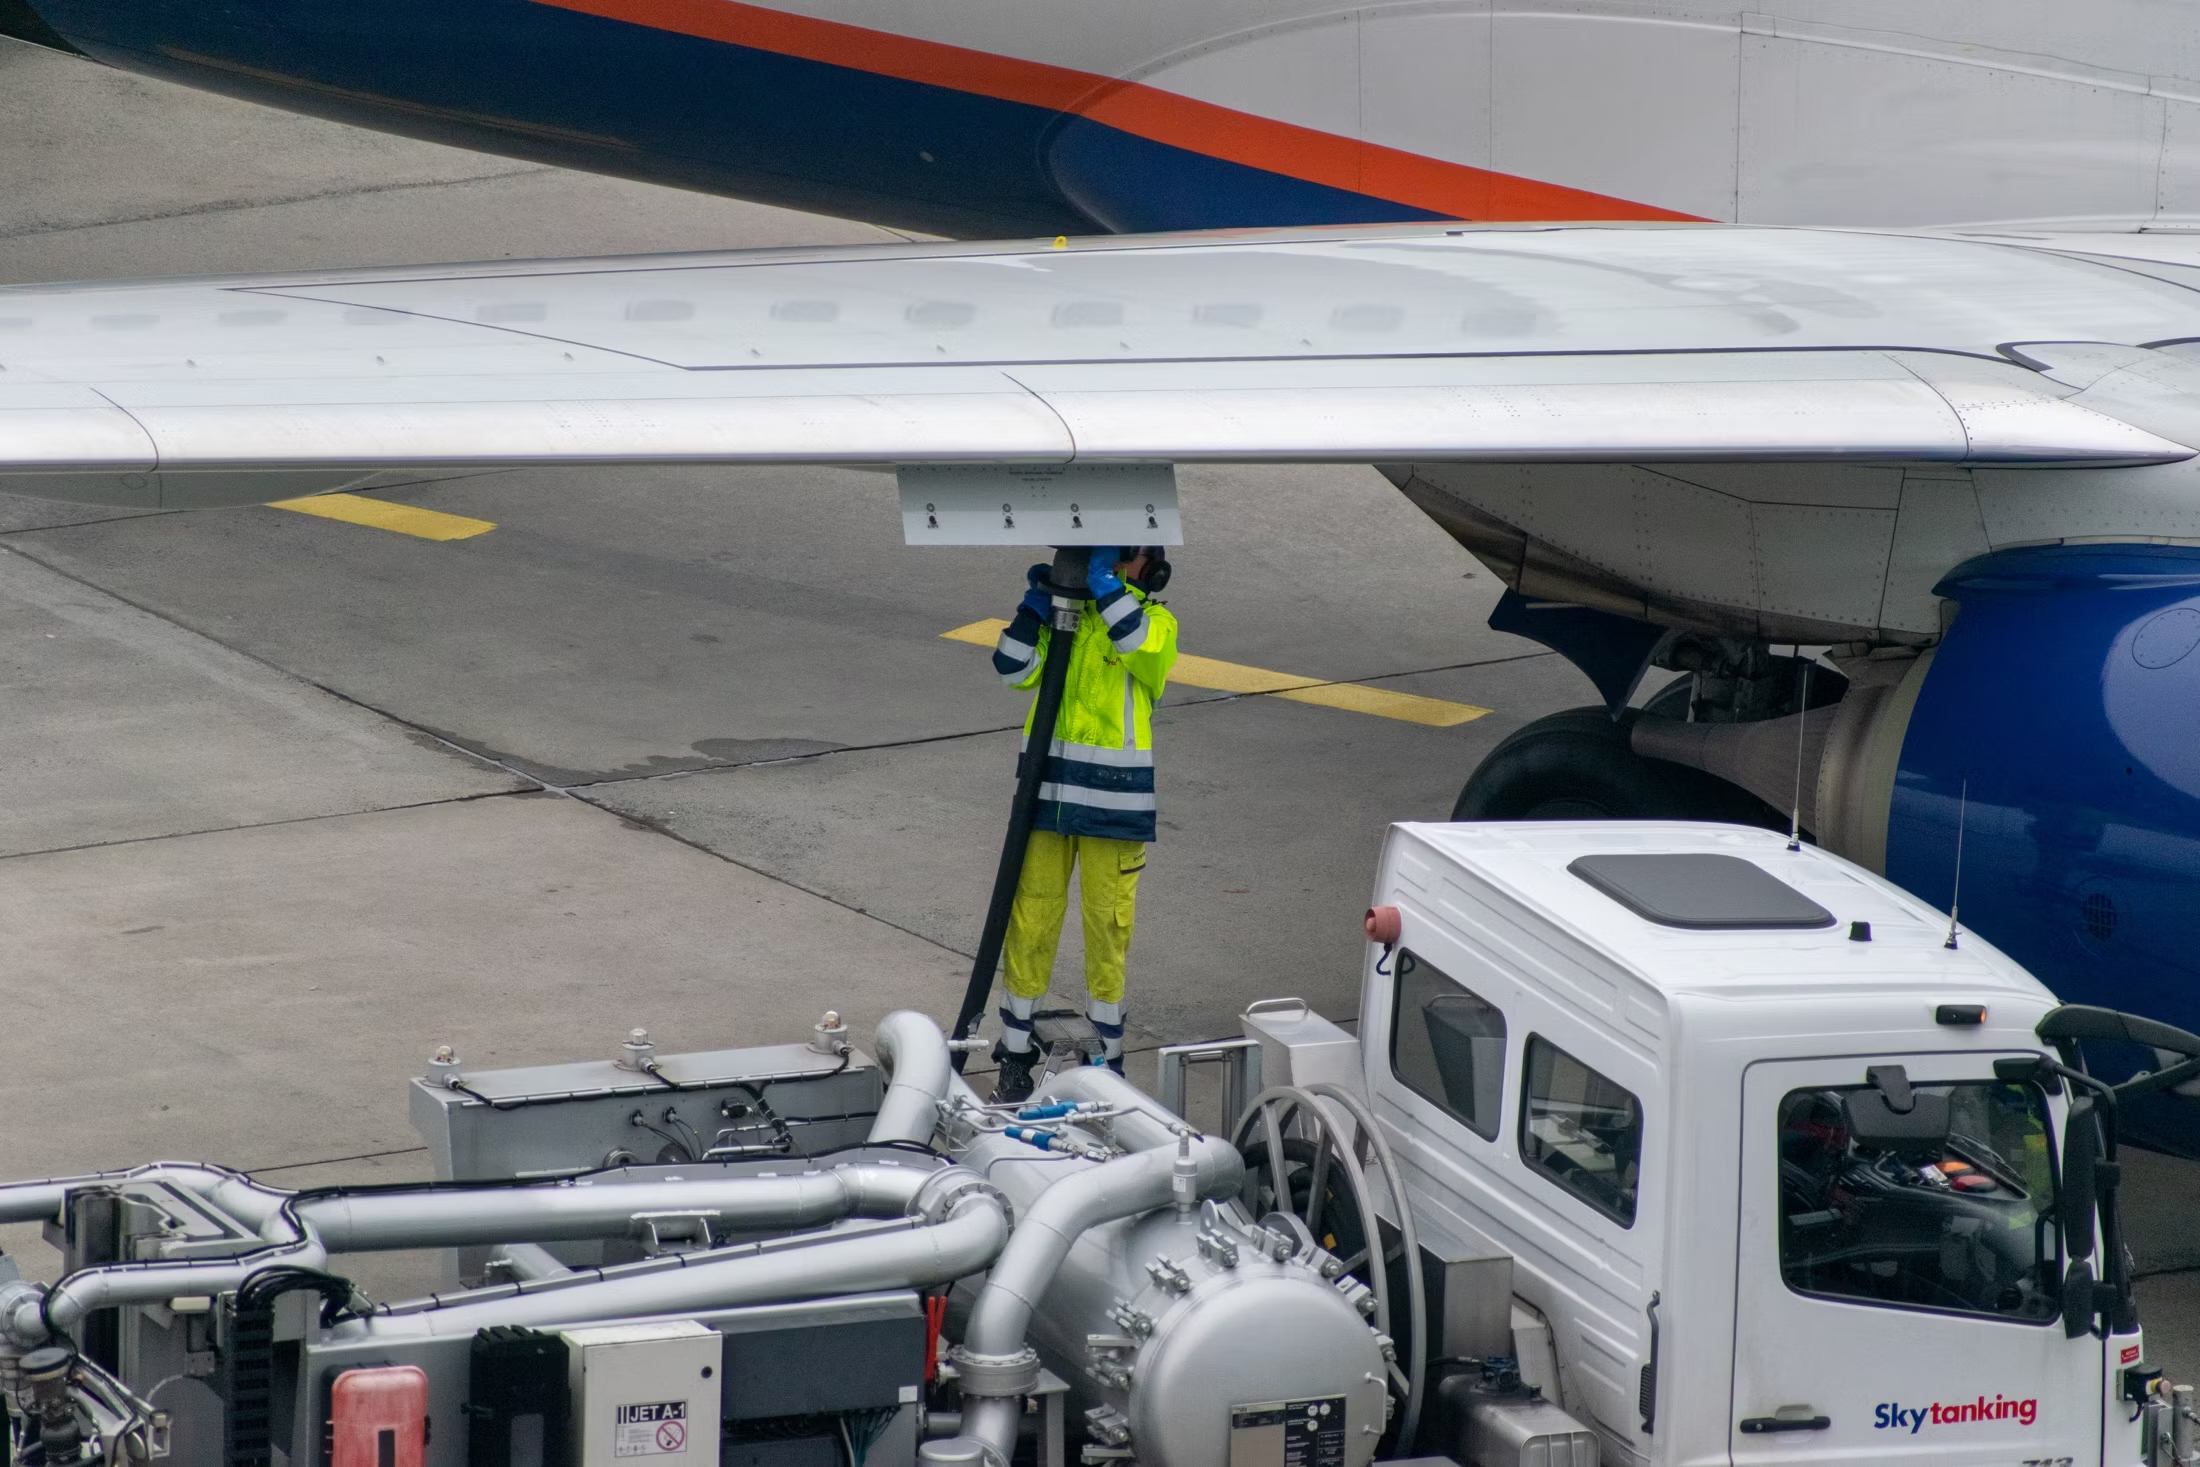
\includegraphics[width=0.5\textwidth]{figures/pressure-refuelling.jpeg}
    \caption{Pressure Refuelling of a Commercial Aircraft. Source: Tom Boon/Simple Flying}\label{fig:pressure-refuelling}
\end{figure}

The aviation industry is undergoing a significant transformation with the
development of the airport of the future, commonly known as `Smart Airport’ or,
more recently, `Airport 4.0’. The concept of Smart Airport encompasses the use
of cutting-edge information technologies, such as the Internet of Things (IoT),
Artificial Intelligence (AI), and Blockchain, to monitor, analyse, and
integrate real-time data on the airport's status. This integration aims to
achieve optimal operational efficiency and enhance the quality of service.
Taking the concept a step further, Airport 4.0 envisages an airport driven
entirely by AI, capable of making autonomous decisions thanks to self-learning
mechanisms. This advance aims to automatically predict and manage various
airport scenarios, making it easier to automate numerous processes. The result
is a substantial reduction in operating costs and error
rates~\cite{10.1007/978-981-16-5943-0_26}.

Among these, automated refuelling systems play a crucial role in ensuring
efficient and accurate refuelling of aircraft. However, one of the main
challenges of this automation process is the accurate detection of the
aircraft's refuelling port, which is relatively small and can easily be
obscured by other visual elements on or near an aircraft. For example in the
Figure~\ref{fig:challenges-detecting-ports}, the refuelling port is located on
the wing of the aircraft and can be difficult to detect due to motion blur,
occlusion, or being out of view. This challenge is further compounded by the
fact that aircraft refuelling ports can vary in size, shape, and location
depending on the aircraft type and manufacturer. Scanning the entire area of
each video frame is both time-consuming and inaccurate. It is therefore
essential to develop a more efficient and accurate method of locating the
refuelling port. 

% 4 Images
\begin{figure}[H]
    \centering
    \begin{subfigure}[b]{0.3\textwidth}
        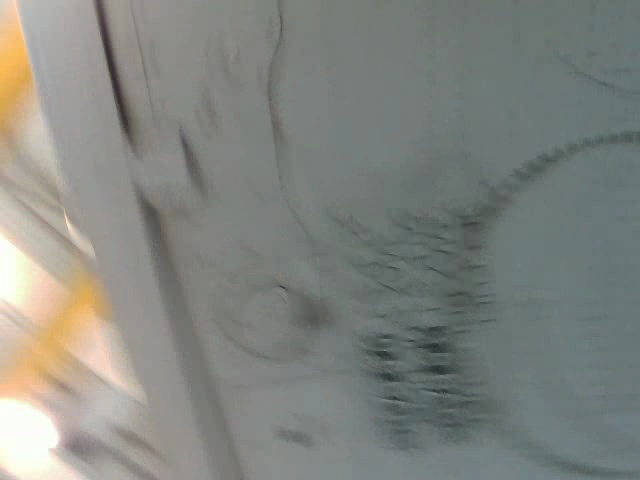
\includegraphics[height=0.7\textwidth, width=\textwidth]{figures/image_hard_2.jpg}
        \caption{Motion Blur Example}\label{fig:motion-blur-example}
    \end{subfigure}
    \hfill
    \begin{subfigure}[b]{0.3\textwidth}
        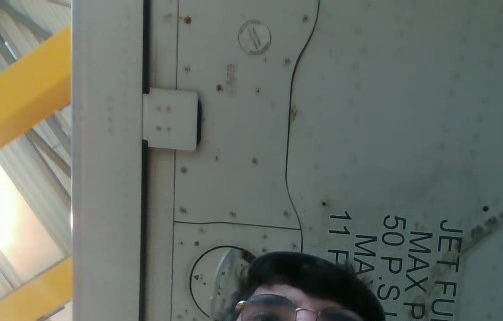
\includegraphics[height=0.7\textwidth, width=\textwidth]{figures/image_hard_4.jpg}
        \caption{Occlusion Example}\label{fig:occlusion-example}
    \end{subfigure}
    \hfill
    \begin{subfigure}[b]{0.3\textwidth}
        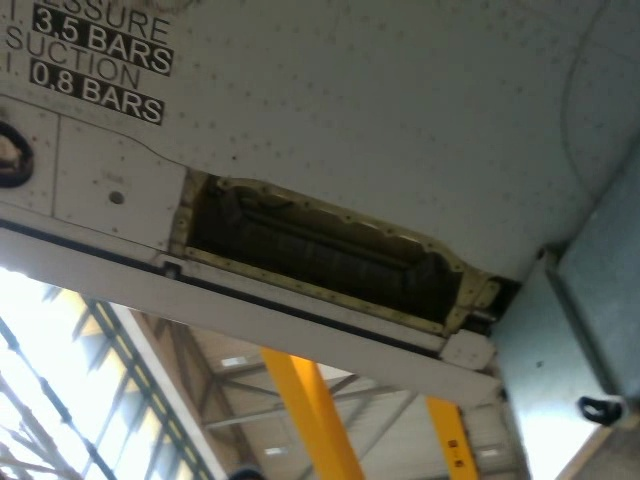
\includegraphics[height=0.7\textwidth, width=\textwidth]{figures/image_hard_3.jpg}
        \caption{Out-of-View Example}\label{fig:out-of-view-example}
    \end{subfigure}
    \caption{Challenges in Detecting Aircraft Refuelling Port}\label{fig:challenges-detecting-ports}
\end{figure}

\section{Research Gap}
Despite significant advancements in autonomous aircraft ground refuelling
technologies, critical challenges remain, particularly in the accurate
detection and positioning of the refuelling port. The small size and varied
locations of refuelling ports, often obscured by visual elements like motion
blur and occlusions, complicate this task. Existing systems have made progress
using machine vision, but they are limited by inefficiencies in scanning entire
video frames and inaccuracies under different environmental conditions.
Furthermore, while current methodologies leveraging convolutional neural
networks (CNNs) and Kalman filters have improved detection accuracy, they still
struggle with real-time performance and adaptability in dynamic environments.
The robustness of these systems in varied lighting conditions and their
capability to handle different refuelling port types and obstructions need
enhancement. Additionally, the application of advanced deep learning models
like Long Short-Term Memory (LSTM) networks, Recurrent Neural Networks (RNNs),
and Transformers in this context is underexplored. 

\newpage

\section{Aim and Objectives}
This thesis aims to address the previous research gaps by developing a
framework for predicting the future position of commercial aircraft refuelling
ports using advanced Object Detection models and Deep Learning to leverage the
spatial-temporal relationship between frames in a video.
\begin{enumerate}
    \item Conduct a comprehensive review of state-of-the-art methods for Object
          Detection, Object Tracking, and Deep Learning Sequence Models.
    \item Annotate and preprocess video datasets of aircraft refuelling ports to ensure
          high-quality training and testing data.
    \item Design and develop a framework for accurately tracking and predicting the
          future position of aircraft refuelling ports.
\end{enumerate}

\section{Technological Contributions}
This thesis makes several technological contributions aimed at advancing the
field of automated aircraft refuelling systems. The primary contribution is the
integration of advanced deep learning models, including Long Short-Term Memory
(LSTM) networks and Gated Recurrent Unit (GRU) networks, to predict the future
positions of refuelling ports by leveraging their superior spatio-temporal data
processing capabilities. Another significant contribution is the development of
an innovative framework that combines object detection, target tracking, and
future position prediction to enhance the accuracy and efficiency of automated
refuelling systems. This framework is designed to handle the small pixel ratio
of refuelling ports efficiently, thus optimising the detection and tracking
process. The use of Extended Kalman Filtering (EKF) further refines
predictions, ensuring real-time adaptability and accuracy, which is crucial for
practical applications in busy airport environments. 

\section{Thesis Layout}
The following sections of this thesis provide a detailed exploration and
analysis of the methodologies, experiments, and findings related to the
development of an advanced framework for predicting the future positions of
aircraft refuelling ports. The Chapter~\ref{chap:literature-review} (Literature
Review) presents an overview of the current state-of-the-art methods in
automated aircraft refuelling systems, object detection, and deep learning for
spatio-temporal prediction. The Chapter~\ref{chap:methodology} (Methodology)
describes the step-by-step approach taken in dataset preparation, framework
design, and model training. The Chapter~\ref{chap:experiment_design}
(Experiment Design) outlines the experimental setups and comparison studies
conducted to evaluate the performance of the proposed models. In the
Chapter~\ref{chap:results} (Results and Discussion), the outcomes of these
experiments are presented and analysed, offering insights into the
effectiveness and implications of the research findings. Finally, the
Chapter~\ref{chap:conclusion} (Conclusion and Future Work) summarises the key
contributions of the thesis, reflects on the significance of the results, and
proposes directions for future research to further advance the field of
automated aircraft refuelling systems.

%%%%%%%%%%%%%%%%%%%%%%%%%%%%%%%%%%%%%%%%%%%%%%%%%%%%%%%%%%%%%%%%%%%%%%%%%%%%%%%%

%%%%%%%%%%%%%%%%%%%%%%%%%%%%%%%%%%%%%%%%%%%%%%%%%%%%%%%%%%%%%%%%%%%%%%%%%%%%%%%%
%%%%%%%%%%%%%%%%%%%%%%%%%%%%% LITERATURE REVIEW %%%%%%%%%%%%%%%%%%%%%%%%%%%%%%%%
\chapter{Literature Review}\label{chap:literature-review}
\section{Automated Refulling Systems in the Aviation Industry}
Ground refueling operations are essential to maintaining aircraft availability
and operational efficiency. The transition from manual to automated systems is
designed to improve the safety, efficiency and reliability of these
operations~\cite{ExpertSystemsAGR}. The concept of Autonomous Aircraft Ground
Refueling (AAGR) emerged in the 1980s in the United States to address the US
Air Force’s need to protect ground personnel from potential threats during
refueling operations~\cite{Schultz1986}. In the early 1990s,
\citet{Bennett1991} introduced the Brightness Invariant Port Recognition System
(BIPRS), marking a significant advancement in machine vision systems for
identifying aircraft refuelling ports. In 2010, the Air Force Research
Laboratory (AFRL) showcased the world’s first Automated Aircraft Ground
Refuelling system prototype through a video demonstration. This system featured
a robot equipped with a fuel nozzle and a single-point refuelling adapter,
enabling autonomous engagement with the aircraft's refuelling panel, as
illustrated in Figure~\ref{fig:test-2010} \cite{Burnette2010}. This project
will give birth to the Autonomous \& Robotic Remote Refuelling Point (AR3P)
project.

\begin{figure}[H]
    \centering
    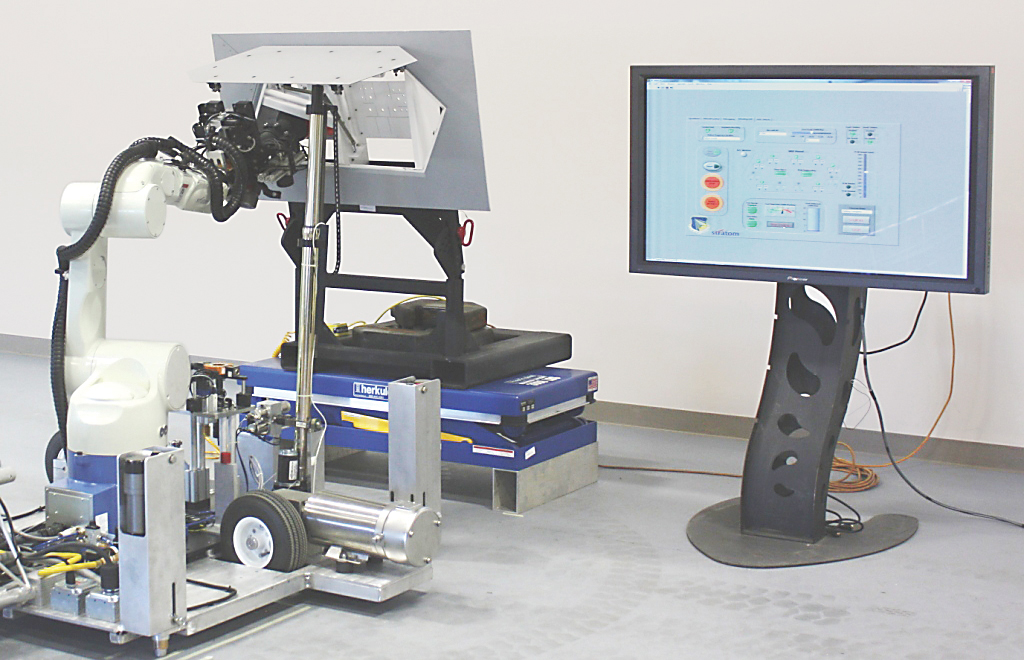
\includegraphics[width=0.6\textwidth]{figures/test_2010.jpeg}
    \caption{AFRL's Automated Aircraft Ground Refueling system prototype robot (Photo Credit: AFRL/RXQ Robotics Group)}\label{fig:test-2010}
    \label{fig:test-2010}
\end{figure}

The Autonomous \& Robotic Remote Refuelling Point (AR3P) project, developed by
the U.S. Army, represents a pioneering initiative in unmanned refuelling
operations for rotary-wing aircraft. This project leverages advanced robotics,
including self-aligning mechanisms and articulated arms equipped with sensors,
to facilitate rapid and safe refuelling processes on non-contiguous
battlefields. The AR3P system minimises the time aircraft spend on the ground
and enhances safety by reducing soldier exposure at fueling stations. Initially
demonstrated in a Limited Initial Capabilities event, the AR3P aims to meet the
evolving range and endurance requirements of Army Aviation. The project
integrates existing technologies with novel systems designed in-house,
supported by commercial off-the-shelf components and additive manufacturing.
Currently, AR3P is progressing through its development phases, addressing
technical risks, and preparing for further testing and eventual deployment, as
shown in Figure~\ref{fig:test-2017} \cite{Ficken2017}.

\begin{figure}[H]
    \centering
    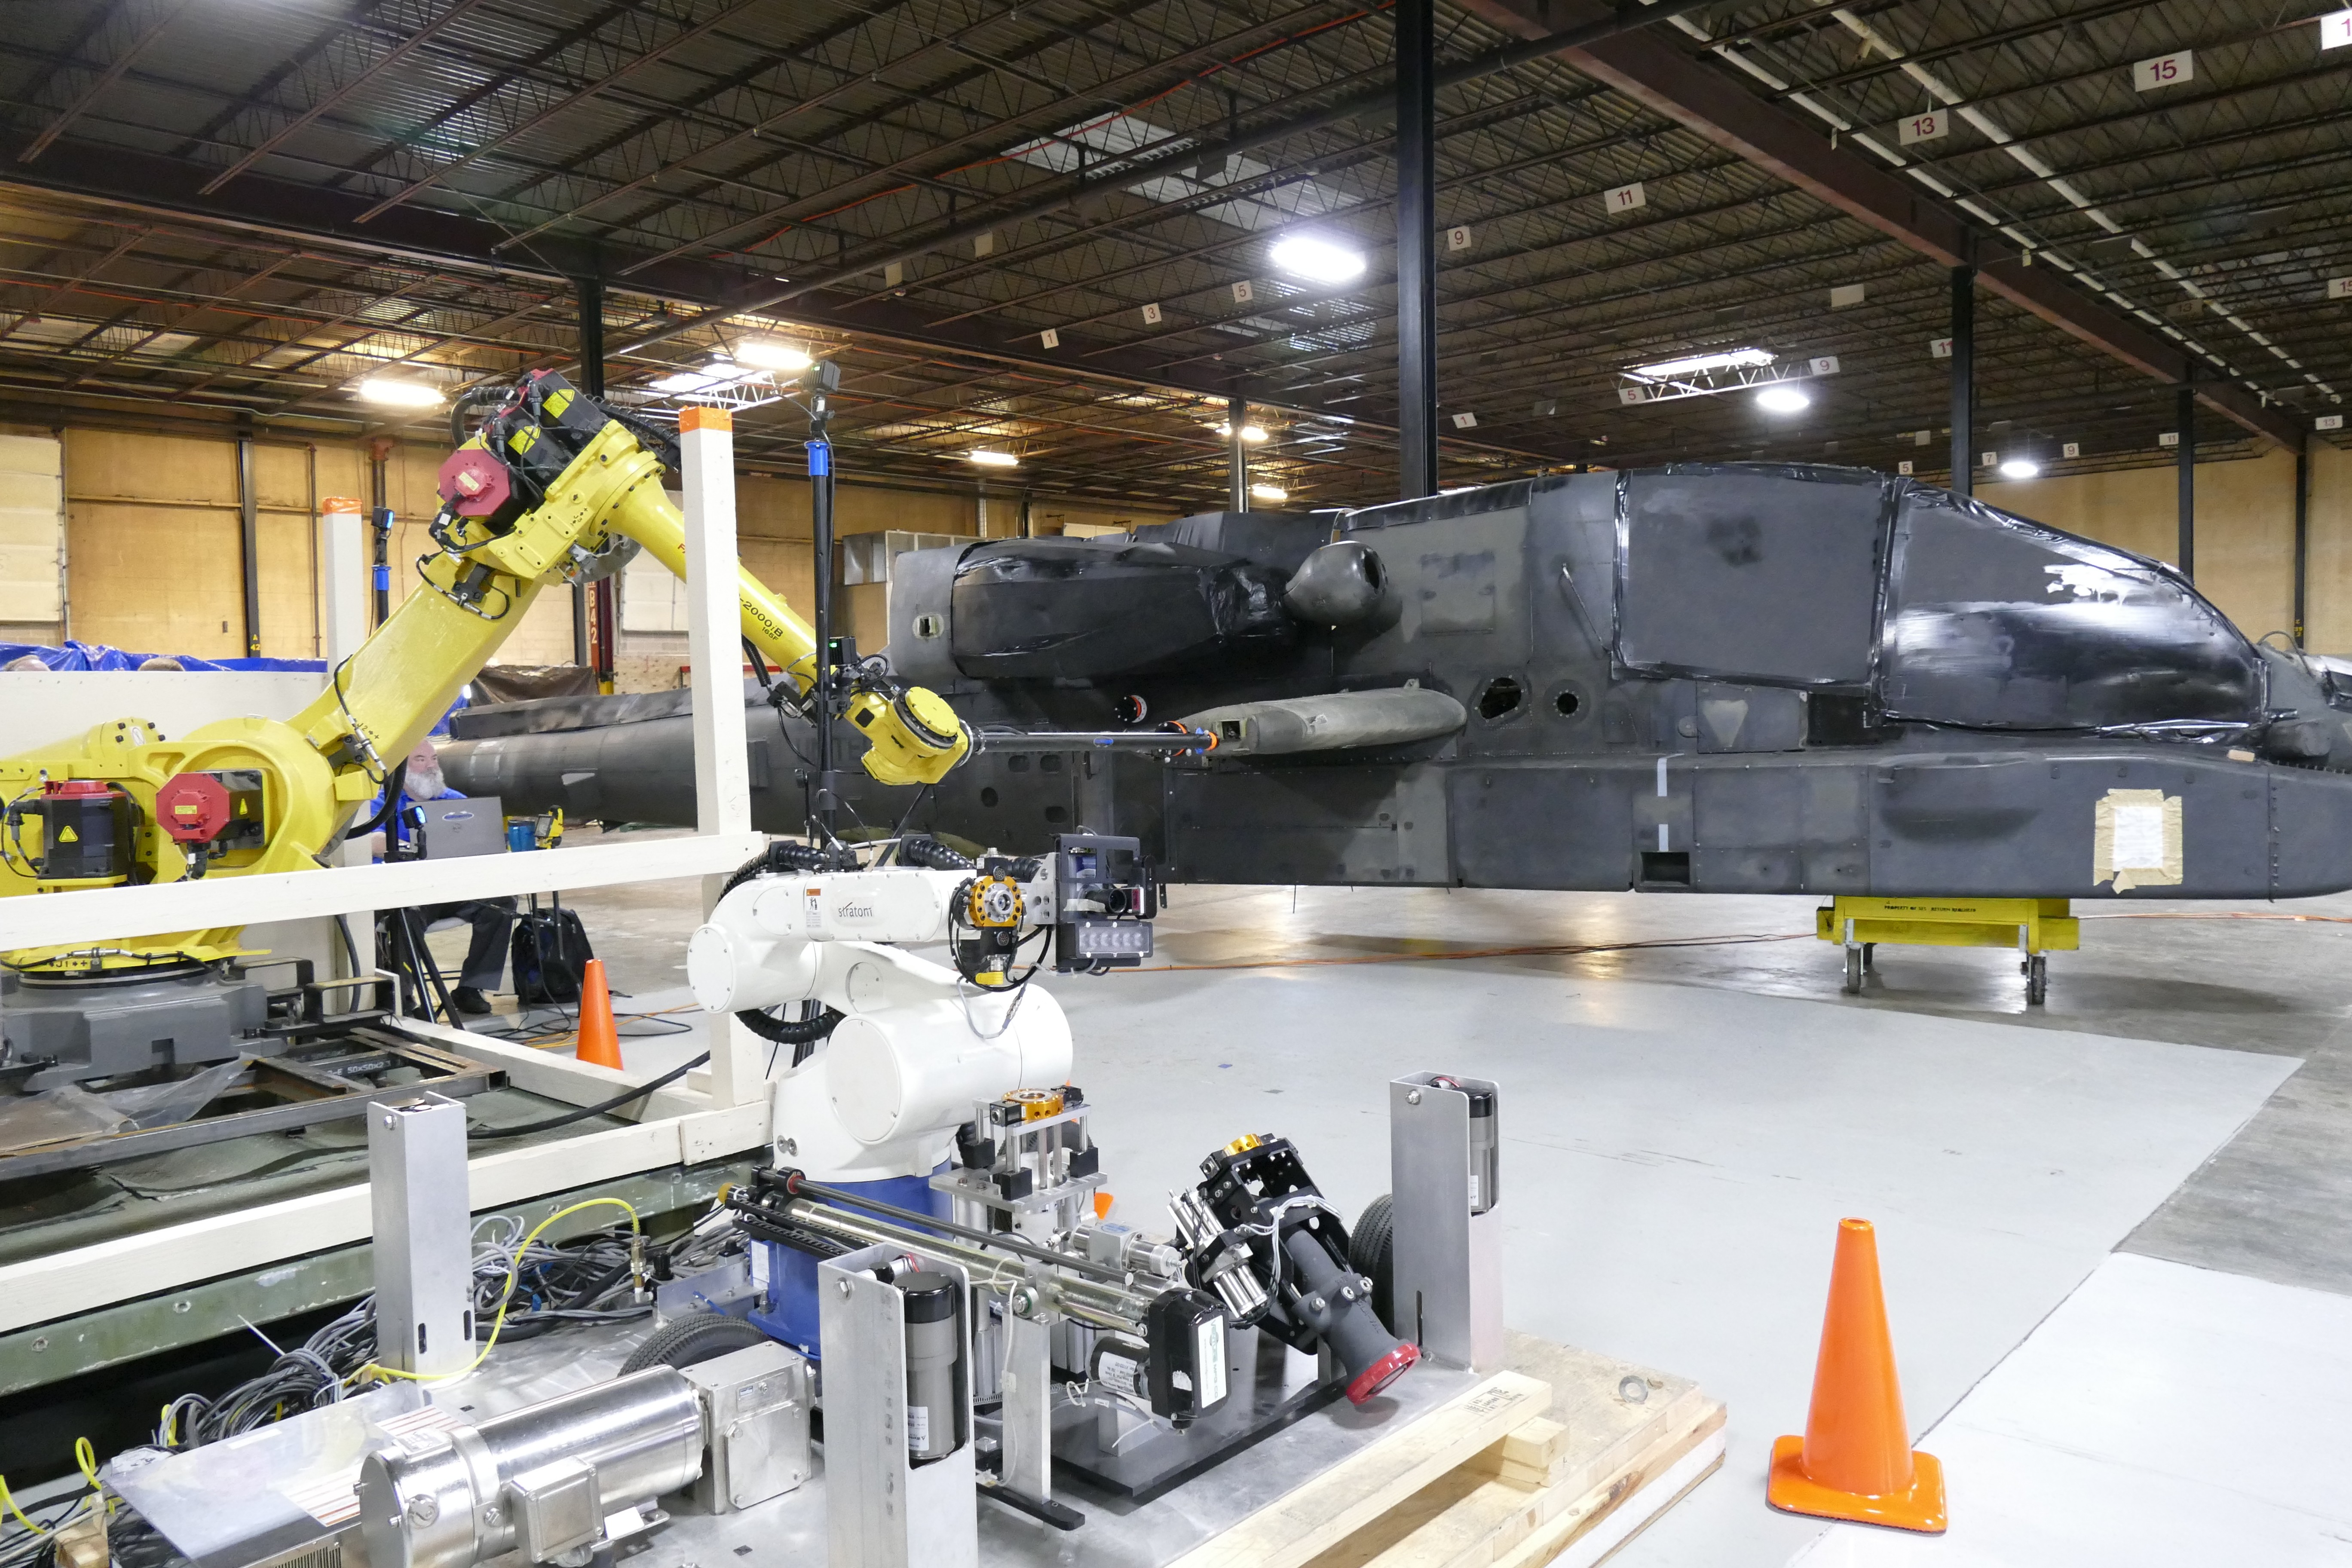
\includegraphics[width=0.5\textwidth]{figures/test_2017.jpg}
    \caption{AR3P Concept Development Prototype Robot (Photo Credit: U.S. Army)}\label{fig:test-2017}
\end{figure}

The AR3P project exemplifies the intersection of advanced robotics and
practical military applications, highlighting the potential of automated
systems to transform operational paradigms.
Figure~\ref{fig:automated-refuelling-systems} provides visual insights into the
capabilities of the AR3P system, by performing autonomous hot refuelling.
During this test, the robot is equipped with a LIDAR sensor and a camera to
detect the aircraft's refuelling port. In Figure~\ref{test-2020-2}, the AR3P
robot is seen approaching a detected aircraft, demonstrating its autonomous
navigation and alignment capabilities. In Figure~\ref{test-2020-3}, the AR3P
robot is shown engaging the aircraft refuelling port, emphasising its precision
and functionality in connecting to the aircraft’s fuel port. These images
illustrate the practical implementation of robotic technologies in enhancing
the safety, efficiency, and speed of refuelling operations, particularly in
challenging and hazardous environments \cite{AR3P2020}.

\begin{figure}[H]
    \centering
    \begin{subfigure}[b]{0.45\textwidth}
        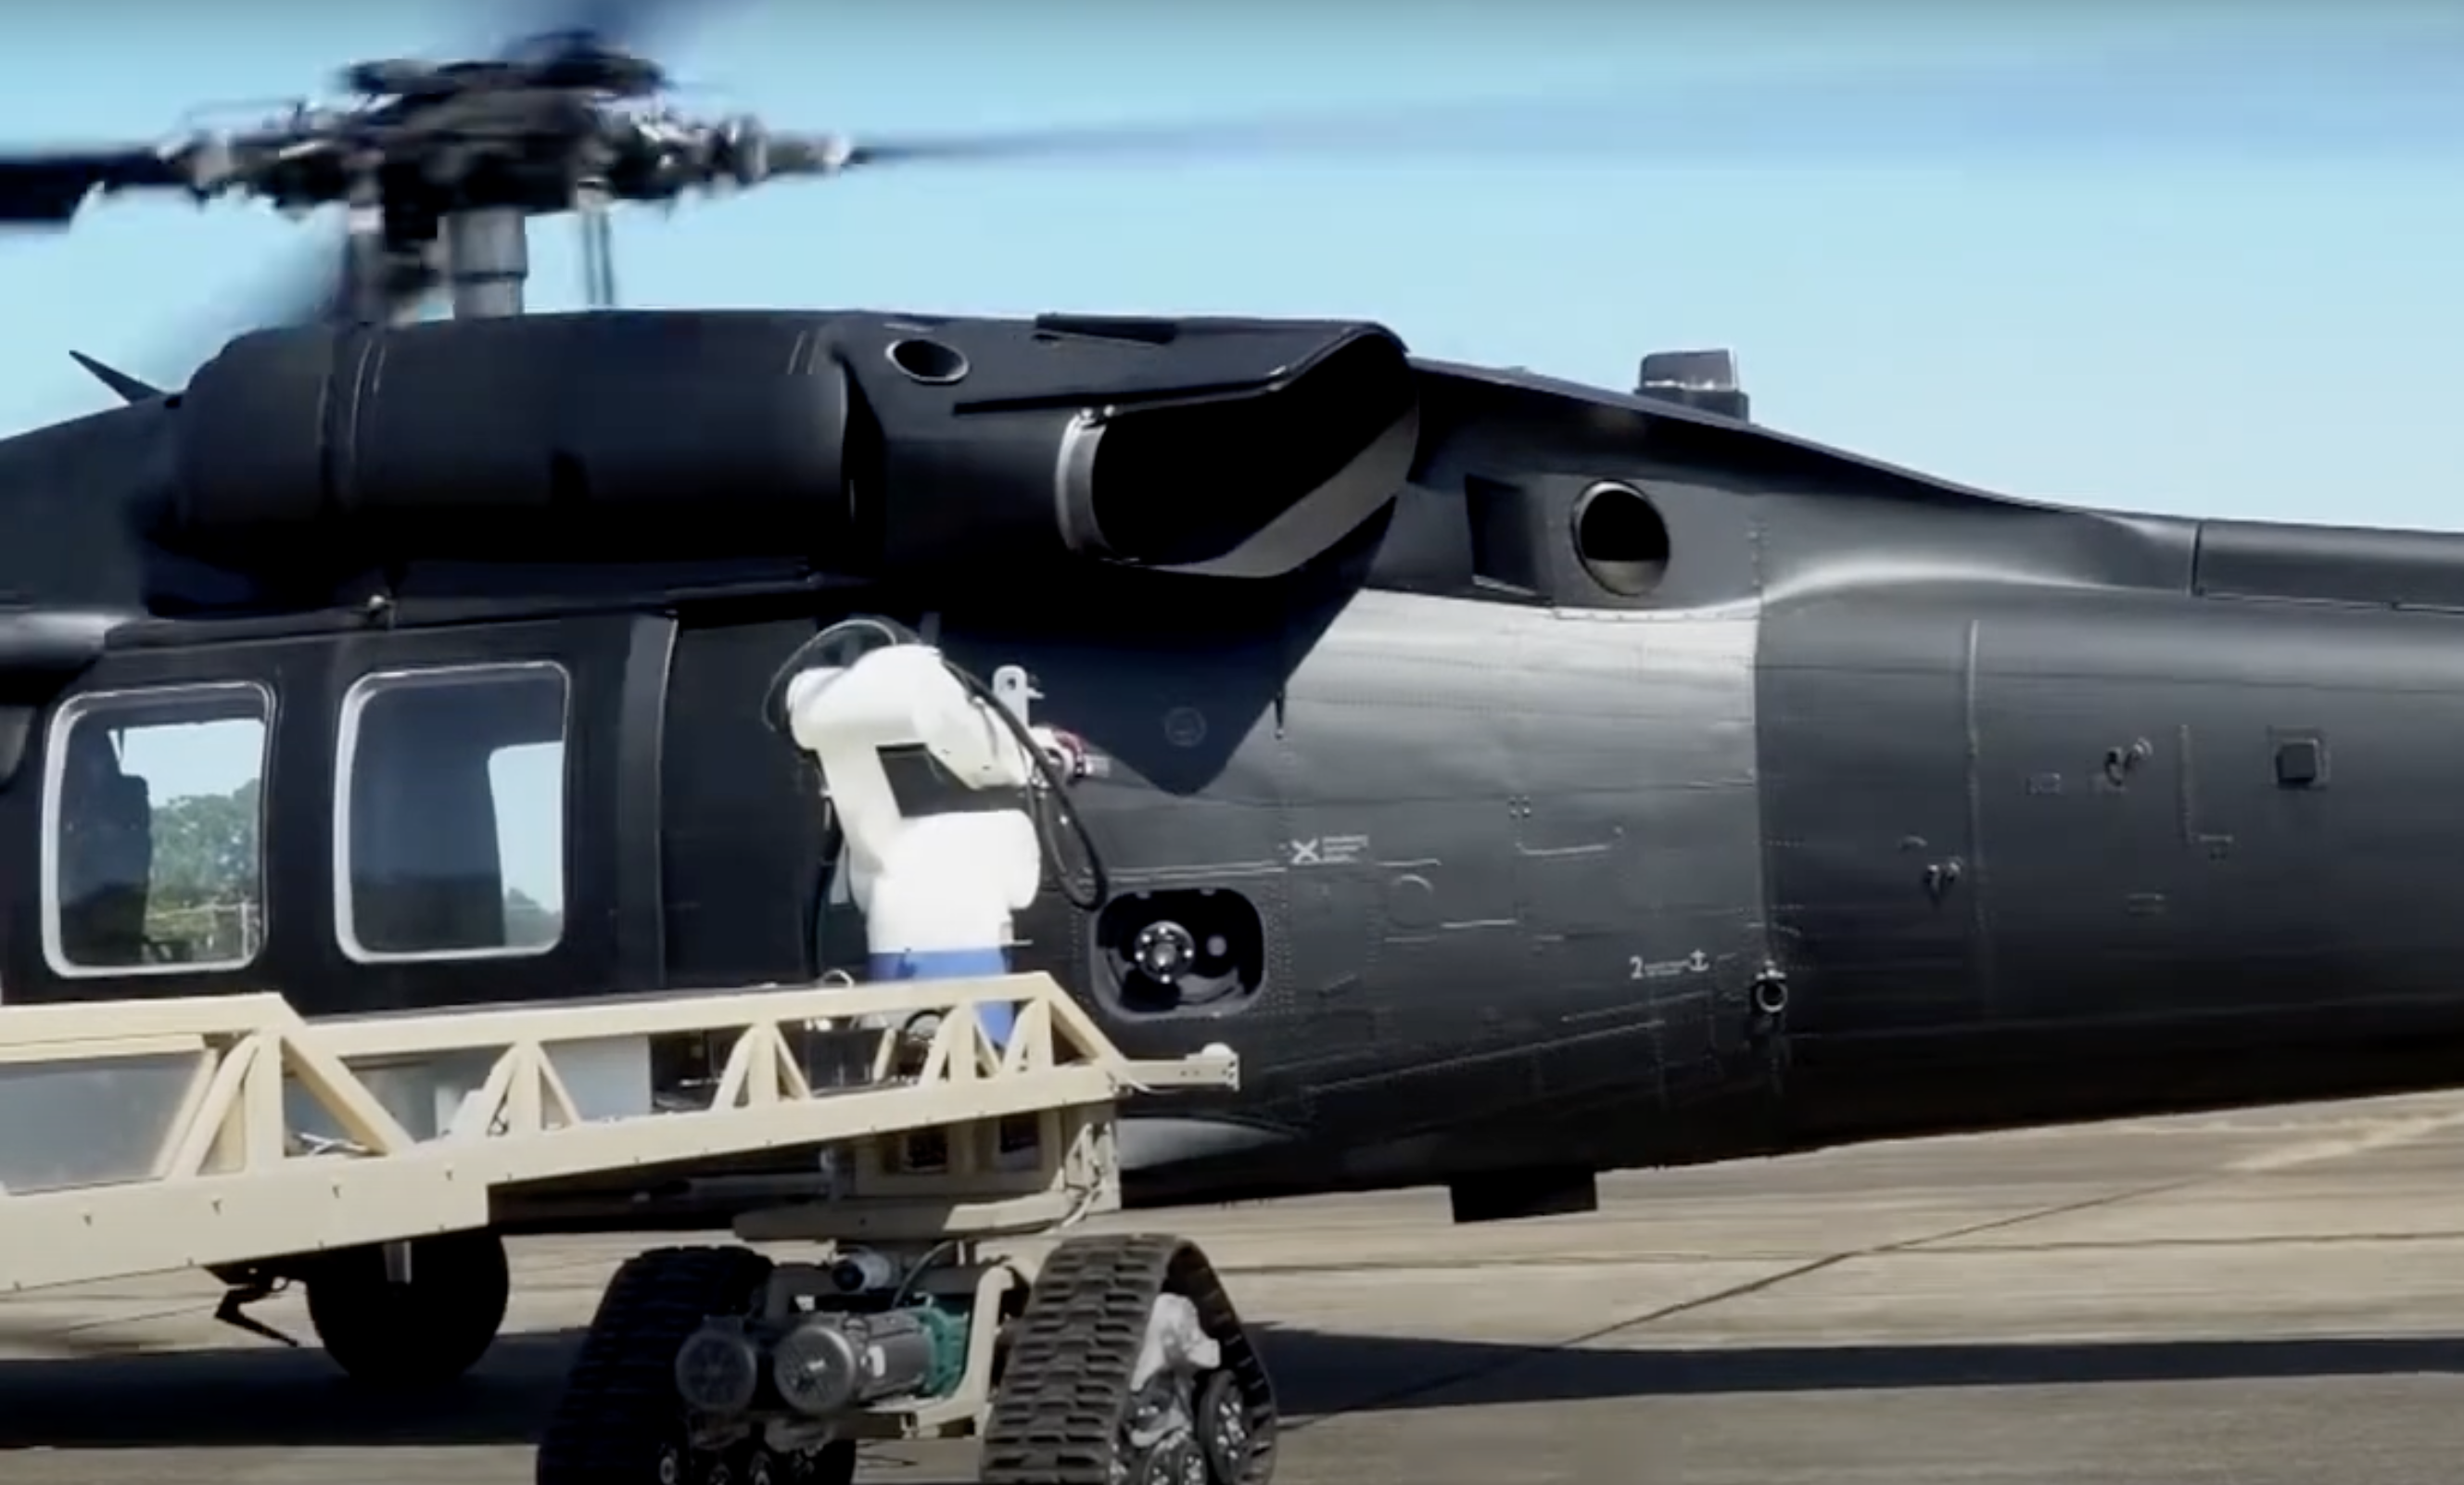
\includegraphics[height=0.68\textwidth, width=\textwidth]{figures/test_2020_2.png}
        \caption{AR3P Robot Approaching Detected Aircraft (Photo Credit: Stratom)}\label{test-2020-2}
    \end{subfigure}
    \hfill
    \begin{subfigure}[b]{0.45\textwidth}
        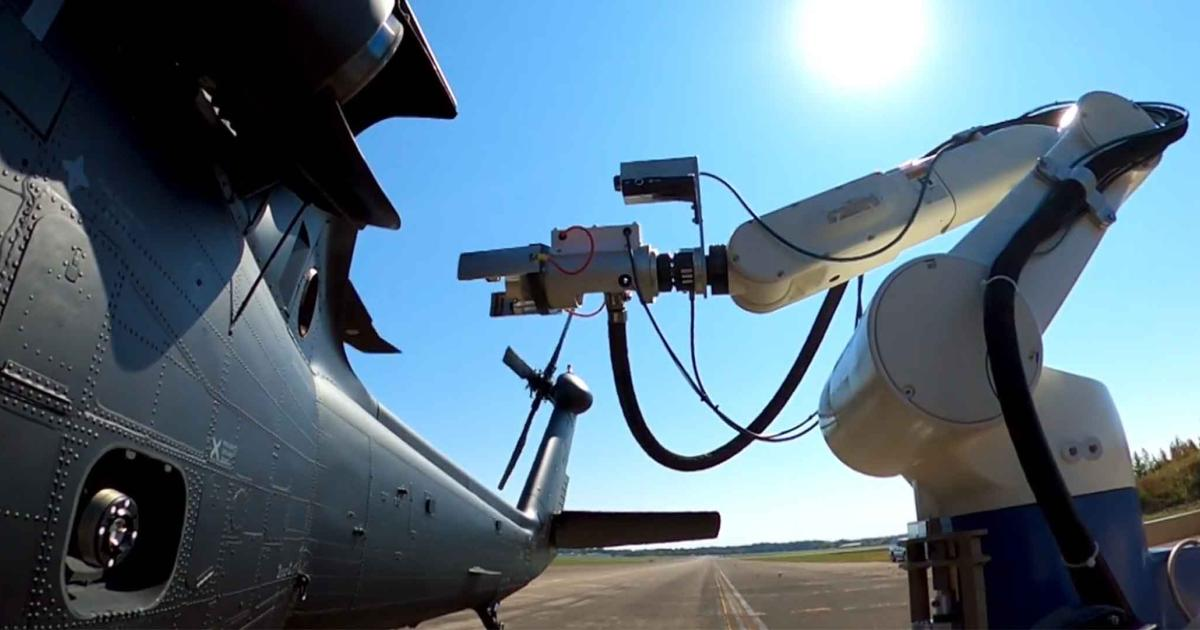
\includegraphics[height=0.68\textwidth, width=\textwidth]{figures/test_2020_3.jpg}
        \caption{AR3P Robot Engaging Aircraft Refueling Port (Photo Credit: Stratom)}\label{test-2020-3}
    \end{subfigure}
    \caption{AR3P Robot Hot Refueling Demonstration for S-70 Helicopter}\label{fig:automated-refuelling-systems}
\end{figure}

\newpage

Unfortunately, there is very little literature on existing AAGR systems, as
most research is carried out by the military and is classified. The most recent
papers cover Autonomous Aerial Refueling (AAR) systems, which are used to
refuel unmanned aerial vehicles (UAVs) in mid-air. These systems are designed
to extend the flight time and range of UAVs by enabling them to refuel without
landing. AAR systems are particularly challenging due to the high speeds and
altitudes involved, as well as the need for precise measurement and tracking of
the relative position between the receiver aircraft and the tanker aircraft are
critical, particularly during the docking phase (see
figure~\ref{fig:aerial-refuelling})~\cite{AARBinocularVision,
    AARCNN}.~\citet{AAREKF} propose a robust solution that utilises monocular
vision combined with an extended Kalman filter (EKF) to address this challenge.
By implementing EKF, the system can provide reliable position estimations and
track the drogue within a specified region of interest (ROI), even in the
presence of disturbances such as air turbulence. As shown in
figure~\ref{fig:detection-system-aarekf}, this system initialises the state and
covariance matrices, predicts the drogue's position, updates the state based on
new measurements, and continuously refines the ROI for subsequent image
processing. This approach significantly reduces the processing time and
improves the detection frequency from 10 Hz to up to 30 Hz by focusing
computational resources on the predicted ROI. 

\begin{figure}[H]
    \centering
    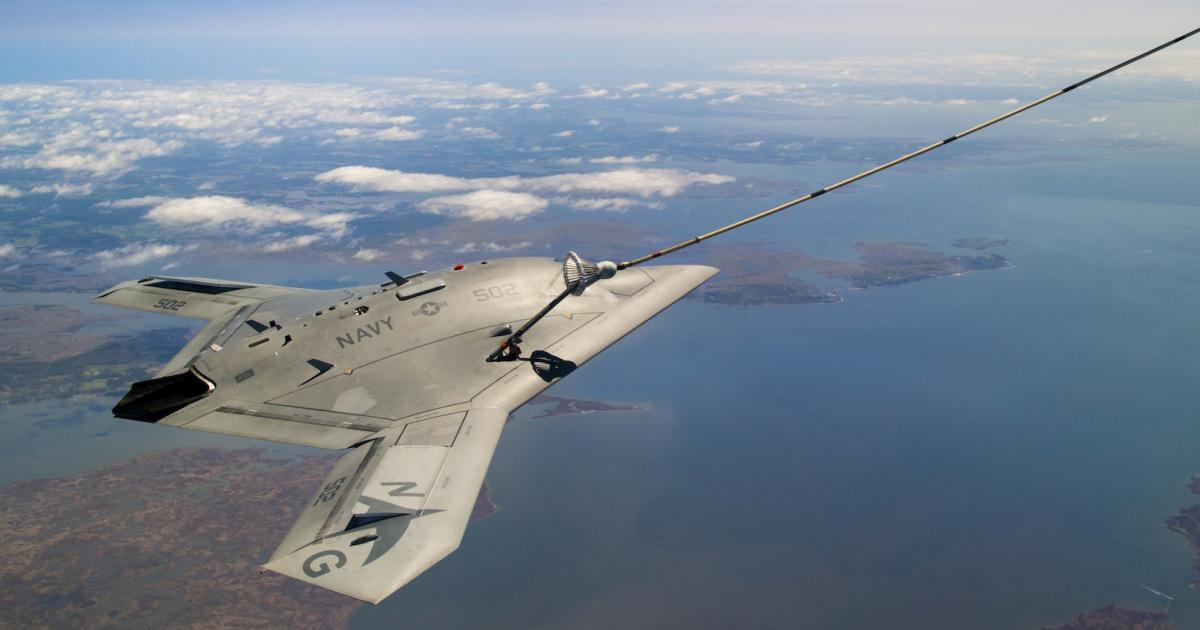
\includegraphics[width=0.5\textwidth]{figures/x-47brefueling.jpg}
    \caption{Autonomous Aerial Refueling (AAR) of X-47B Unmanned Combat Air System Demonstrator (Photo Credit: U.S. Navy)}\label{fig:aerial-refuelling}
\end{figure}

\begin{figure}[H]
    \centering
    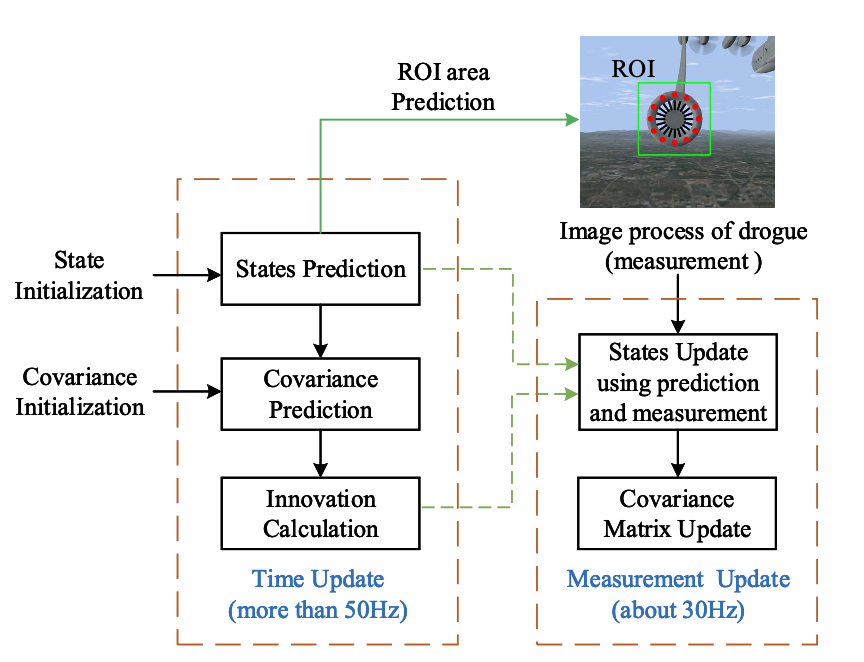
\includegraphics[width=0.6\textwidth]{figures/detection_system_AAREKF.png}
    \caption{Autonomous Air Refueling Detection System with EKF. Source: \citet{AAREKF}}\label{fig:detection-system-aarekf}
\end{figure}

\newpage
Recent advancements in autonomous ground refuelling have been driven by
improvements in computer vision and robotics.~\citet{AGRPoseEstimation}
presented the PosEst system, which combines 2D RGB images with 3D point cloud
data to enhance detection accuracy. This system uses a custom-trained
EfficientNet-B0 CNN for object detection and leverages the Kalman filter for
stable 3D pose estimation (see Figure~\ref{fig:agr-pose-kalman}). The PosEst
method employs a dual approach of high-precision detection and robust tracking.
By predicting and updating the object’s state in real-time, the Kalman filter
facilitates continuous and precise alignment of the fuel nozzle with the
refuelling adaptor, even in dynamic environments. This approach significantly
reduces the risks associated with manual refuelling and improves operational
efficiency and safety.

\begin{figure}[H]
    \centering
    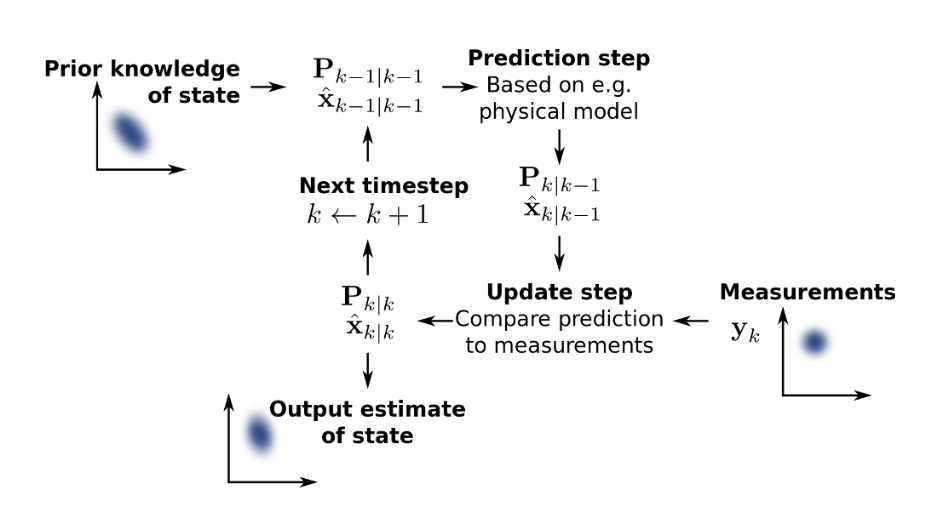
\includegraphics[width=0.45\textwidth]{figures/AGRPoseKalman.png}
    \caption{Kalman Filter Workflow for Pose Estimation in Autonomous Ground Refueling. Source: \citet{AGRPoseEstimation}}\label{fig:agr-pose-kalman}
\end{figure}

One of the primary challenges in AAGR is the accurate detection and positioning
of the refuelling port under varying environmental conditions. Robust datasets
for scene recognition and machine learning applications have been developed to
address these challenges.~\citet{DatasetAGR} introduced a comprehensive dataset
for AAGR, addressing significant challenges such as variant illumination
conditions, different refuelling port types, and environmental obstructions.
The dataset comprises over 26,000 labeled images collected through image
crawling from 13 different databases, followed by augmentation to ensure
diversity (see Figure~\ref{fig:agr-dataset}). Additionally, recent innovations
have introduced hybrid datasets combining real and synthetic data for training
and validating systems \cite{HybridDatasetAGRV1}. This approach offers a wide
range of scenarios and conditions, improving the robustness and accuracy of
automated refuelling systems. The development of high-quality datasets is
pivotal in improving the robustness and reliability of AAGR systems.

\begin{figure}[H]
    \centering
    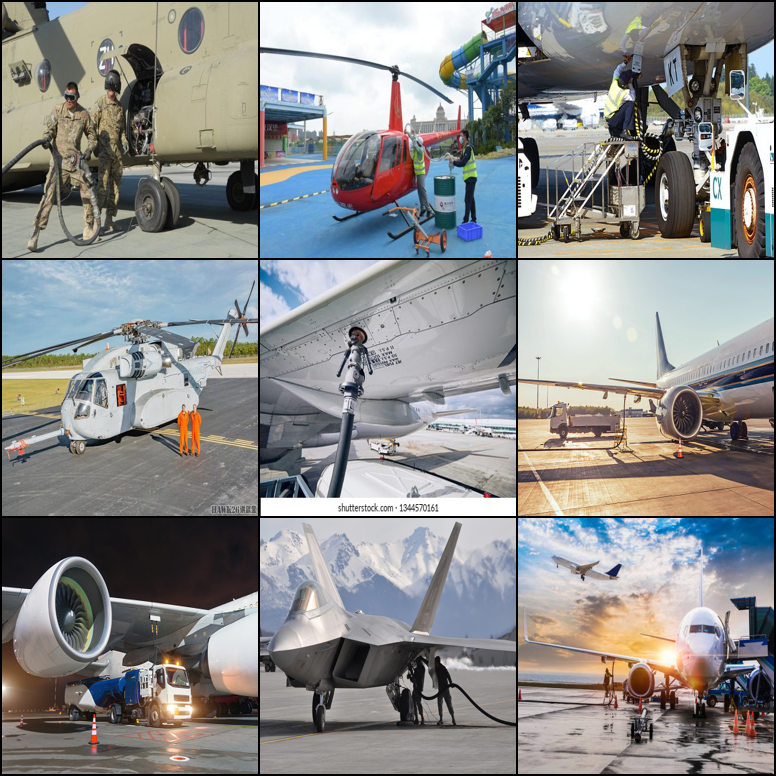
\includegraphics[width=0.4\textwidth]{figures/AGRDatasetGrid.png}
    \caption{AAGR Dataset Overview. Source: \citet{DatasetAGR}}\label{fig:agr-dataset}
\end{figure}

%%%%%%%%%%%%%%%%%%%%%%%%%%%%%%%%%%%%%%%%%%%%%%%%%%%%%%%%%%%%%%%%%%%%%%%%%%%%%%%%

\newpage
\section{Object Detection and Tracking in Computer Vision}
In Computer Vision, Object Detection refers to the identification and location
of individual objects within an image, providing both spatial information
(bounding boxes) and confidence scores, which represent the probability that
each detected object belongs to the predicted
class~\cite{huggingface2023objectdetection}. For example, in the following
image, there are five detections, including one `ball' with a confidence level
of 98\% and four `people' with confidence levels of 98\%, 95\%, 97\% and 97\%.

\begin{figure}[H]
    \centering
    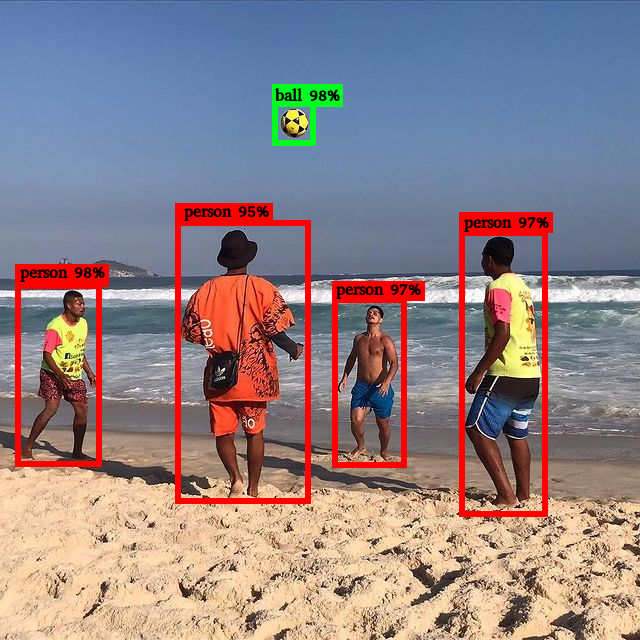
\includegraphics[width=0.3\textwidth]{figures/intro_object_detection.png}
    \caption{Example of outputs from an object detector~\cite{huggingface2023objectdetection}.}\label{fig:object-detection}
\end{figure}

Over the last few decades, Object Detection models based on Deep Learning have
enjoyed remarkable success. These models fall into two main categories:
two-stage detectors and single-stage detectors. On the one hand, two-stage
detectors, such as R-CNN~\cite{DBLP:journals/corr/GirshickDDM13}, Fast
R-CNN~\cite{DBLP:journals/corr/Girshick15}, Faster R-CNN~\cite{Ren2017} and
R-FCN~\cite{DBLP:journals/corr/DaiLHS16}, first generate region proposals and
then refine these proposals into precise anchor boxes. While these models excel
in detection accuracy, they typically suffer from large model sizes and slower
detection speeds~\cite{SurveyDLOD, ODNetworkUAVCNNTransformer}. On the other
hand, single-stage detectors, including the SSD (Single Shot Multibox
Detector)~\cite{DBLP:journals/corr/LiuAESR15}, YOLO (You Only Look Once)
series~\cite{DBLP:journals/corr/RedmonDGF15, DBLP:journals/corr/RedmonF16,
    DBLP:journals/corr/abs-2004-10934, chen2023yoloms,
    DBLP:journals/corr/abs-2107-08430, YOLOv5Release, li2023yolov6, YOLOv8,
    wang2024yolov9, xu2022ppyoloe, wang2023goldyolo, xu2023damoyolo,
    wang2024yolov10}, and RetinaNet~\cite{lin2018focal} directly predict object
locations and categories in a single network pass. These models are known for
their high detection speeds but sometimes compromise accuracy~\cite{SurveyDLOD,
    ODNetworkUAVCNNTransformer}.

\begin{figure}[H]
    \centering
    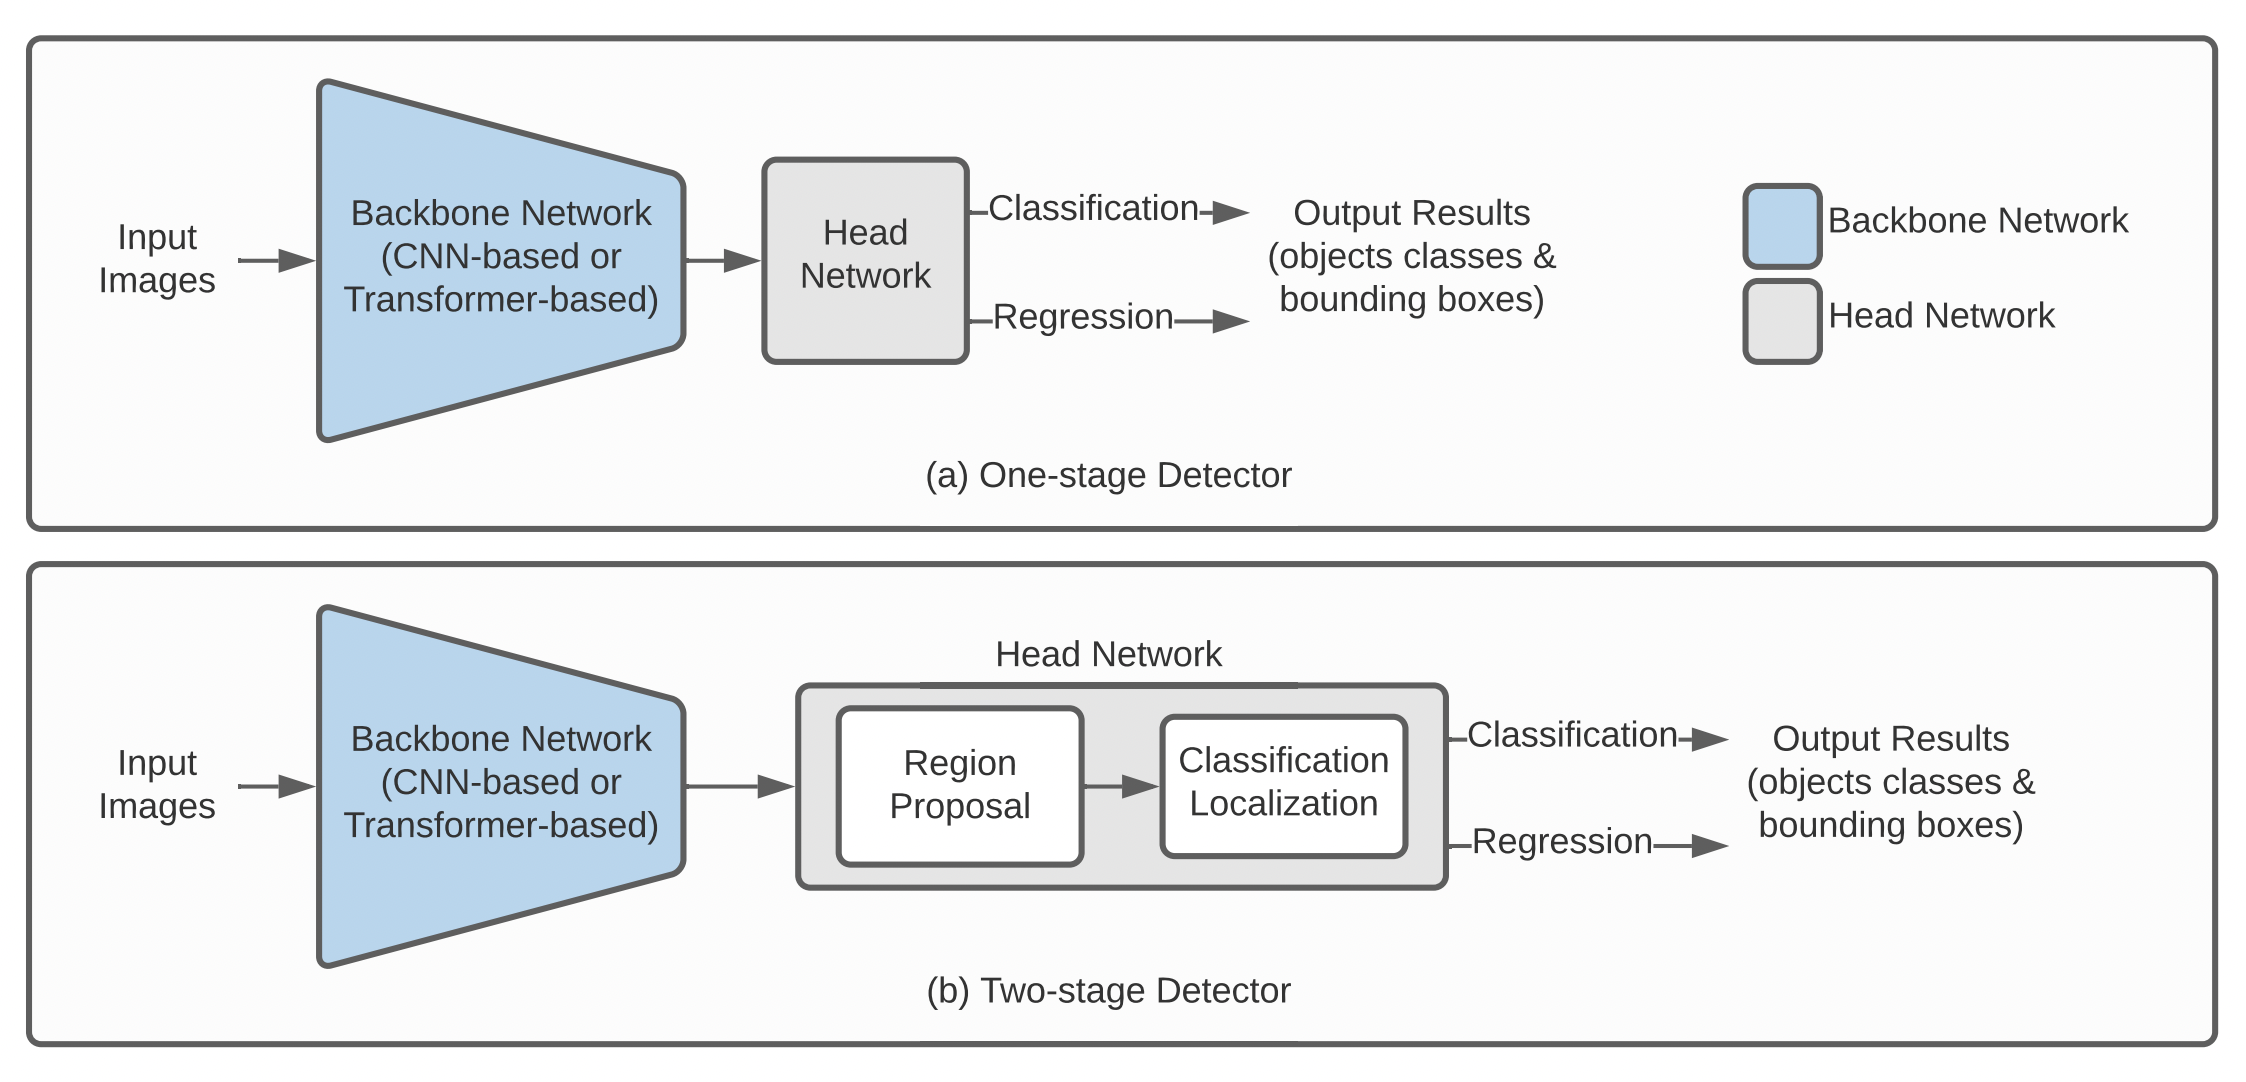
\includegraphics[width=0.8\textwidth]{figures/one-stage_two-stage_OD.png}
    \caption{Basic deep learning-based one-stage vs two-stage object detection model architectures~\cite{SurveyDLOD}.}\label{fig:two-stage-vs-single-stage}
\end{figure}

Evaluating Object Detection models involves several key metrics to measure
their performance. One common metric is Intersection over Union (IoU), which
measures the overlap between a predicted bounding box and a ground-truth
bounding box, as shown in Figure~\ref{fig:iou-metric}.

\begin{figure}[H]
    \centering
    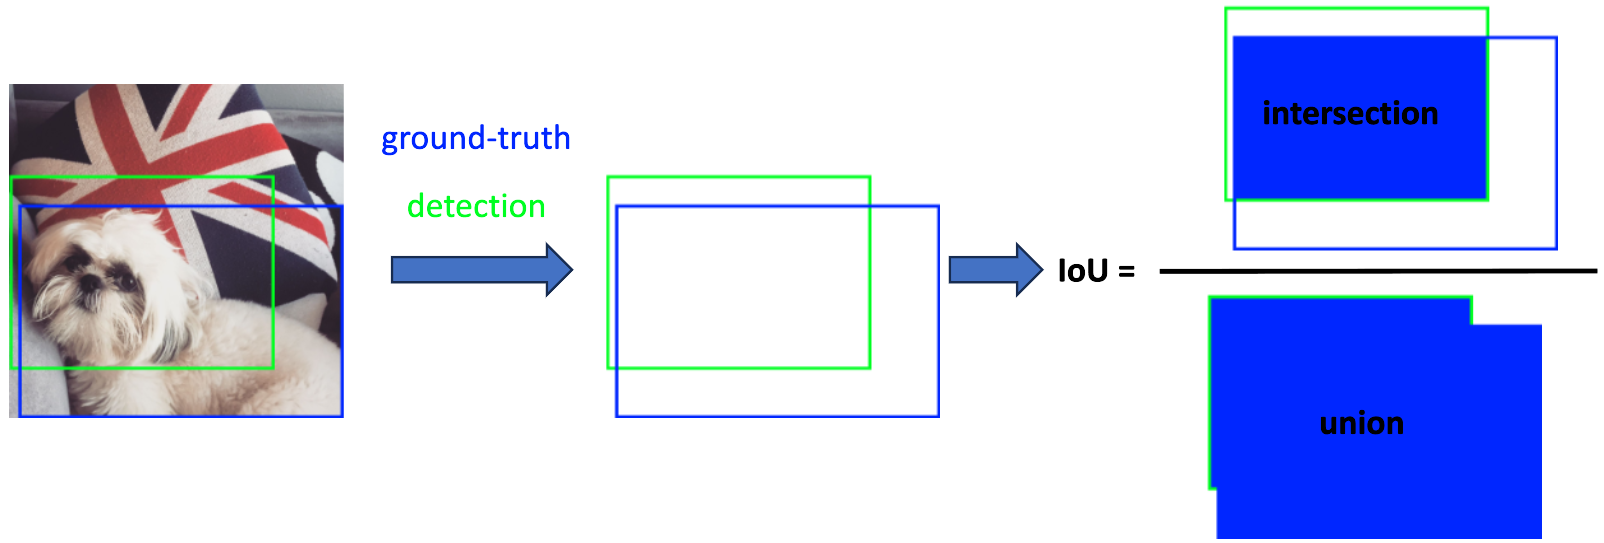
\includegraphics[width=0.8\textwidth]{figures/iou.png}
    \caption{Intersection over Union (IoU) between a detection (in green) and ground-truth (in blue).~\cite{huggingface2023objectdetection}}\label{fig:iou-metric}
\end{figure}

Based on the IoU metric, a detection can be classified as a \textbf{True
    Positive (TP)} or a \textbf{False Positive (FP)} depending on whether the IoU
value exceeds a certain threshold ($T_{IoU}$). If the IoU is above the
threshold, the detection is considered correct (TP); otherwise, it is
classified as a False Positive (FP). Additionally, \textbf{False Negatives
    (FN)} refer to ground truth objects not detected by the model, while
\textbf{True Negatives (TN)} are correctly classified background
detections~\cite{huggingface2023objectdetection}. These classifications allow
for the calculation of the following metrics:

\begin{itemize}
    \item \textbf{Precision}: The ratio of True Positives to the total number of
          detections, measuring the model's ability to avoid false positives:
          \begin{equation}
              \text{Precision} = \frac{\text{TP}}{\text{TP} + \text{FP}}
          \end{equation}

    \item \textbf{Recall}: The ratio of True Positives to the total number of ground-truth objects, measuring the model's ability to avoid false negatives:
          \begin{equation}
              \text{Recall} = \frac{\text{TP}}{\text{TP} + \text{FN}}
          \end{equation}
\end{itemize}

Common metrics used to evaluate Object Detection include:

\begin{itemize}
    \item \textbf{Average Precision (AP)}: This combines precision and recall, providing a single figure summarizing the model's performance across different confidence thresholds. Common versions are AP@.5 (with a threshold of 0.5 IoU) and AP@[.5:.05:.95], which calculates the average of AP values over several IoU thresholds~\cite{huggingface2023objectdetection}.
    \item \textbf{Average Recall (AR)}: This measures the recall of the model averaged across multiple IoU thresholds. It can be computed for different numbers of detections per image, such as AR@1, AR@10, etc.~\cite{huggingface2023objectdetection}.
    \item \textbf{Inference Time}: The time taken by the model to process an image, which is critical for applications requiring real-time detection~\cite{huggingface2023objectdetection}.
    \item \textbf{Model Size}: The number of parameters or the size of the model, affecting deployment, especially on devices with limited resources~\cite{huggingface2023objectdetection}.
    \item \textbf{Efficiency}: This considers the trade-off between accuracy and speed, often visualized using the AP vs. inference time curve~\cite{huggingface2023objectdetection}.
\end{itemize}

In addition to Object Detection, Object Tracking is another critical task in
Computer Vision, involving the continuous monitoring of objects across video
frames. Object Tracking methods can be broadly classified into two categories:
\textbf{Generative Trackers} and \textbf{Discriminative
    Trackers}~\cite{SurveyVisualOT}. Generative trackers are capable of handling
challenging scenarios such as occlusion and large-scale variation through
particle sampling strategies, often integrated with various appearance models,
including sparse representation and energy of motion. Discriminative trackers,
by contrast, build robust classifiers using hand-crafted or deep
features~\cite{SurveyVisualOT}. The combination of generative and
discriminative approaches, as well as the integration of deep learning
techniques such as fully revolutionary networks and Transformer models, has led
to significant improvements in object detection
performance~\cite{OverviewCorrelationAlgoOT, SuveyAdvancesSingleOTMethods,
    SurveyModernODModels}. In addition, the speed and computational requirements of
these algorithms are critical factors influencing their practical
applicability~\cite{SuveyAdvancesSingleOTMethods, SurveyModernODModels,
    SurveyTransformersSingleOT}. Advanced techniques in object tracking leverage
both generative and discriminative models to amplify tracking efficacy. The
utilisation of deep trackers has evidenced superior results on public tracking
datasets, attributed to their potent feature extractors, accurate bounding box
regressors, and discriminative classifiers~\cite{SurveyTransformersSingleOT}.
Techniques such as deformable convolution and Transformer models extend
traditional convolution or correlation methodologies to execute global feature
matching, thereby enhancing tracking accuracy. The incorporation of contextual
or knowledge information can substantially elevate performance, with
methodologies like Particle Filtering, also recognised as Sequential Monte
Carlo (SMC) methods, framed as problems of Bayesian inference in state
space~\cite{SurveySmallObjectDetection, SmallObjectDetectionPositonPrediction}.
The extended Kalman Filtering (EKF) is another advanced technique that has been
employed to improve tracking accuracy by predicting the current status through
the previous status and modifying the prediction result based on observation
information~\cite{SuveyAdvancesSingleOTMethods, SurveyModernODModels}. Despite
these advancements, the integration of these methods in a complementary manner
remains an open research area with substantial potential for advancing the
field~\cite{OverviewCorrelationAlgoOT, SuveyAdvancesSingleOTMethods}.

\newpage
\section{Deep Learning for Spacio-Temporal Prediction}
Time series prediction involves processing sequential data to predict future
events or values. Various deep learning models have been applied to this task,
requiring several preparatory steps such as collecting data, designating
attribute types, dealing with inconsistencies and storing datasets. These
datasets are usually classified into units of time such as seconds, minutes and
hours, allowing the construction of metadata for machine
learning~\cite{FFPSpaceSystemVehicles}.

\subsection*{Early Approaches and Models}
The problem of predicting the future locations of objects has been extensively
studied, particularly for static surveillance cameras. Initial efforts utilised
recurrent neural networks (RNNs), including long-term memory networks (LSTMs)
and gated recurrent units (GRUs), in an encoder-decoder format to encode past
observations and decode future locations. 

\begin{figure}[H]
    \centering
    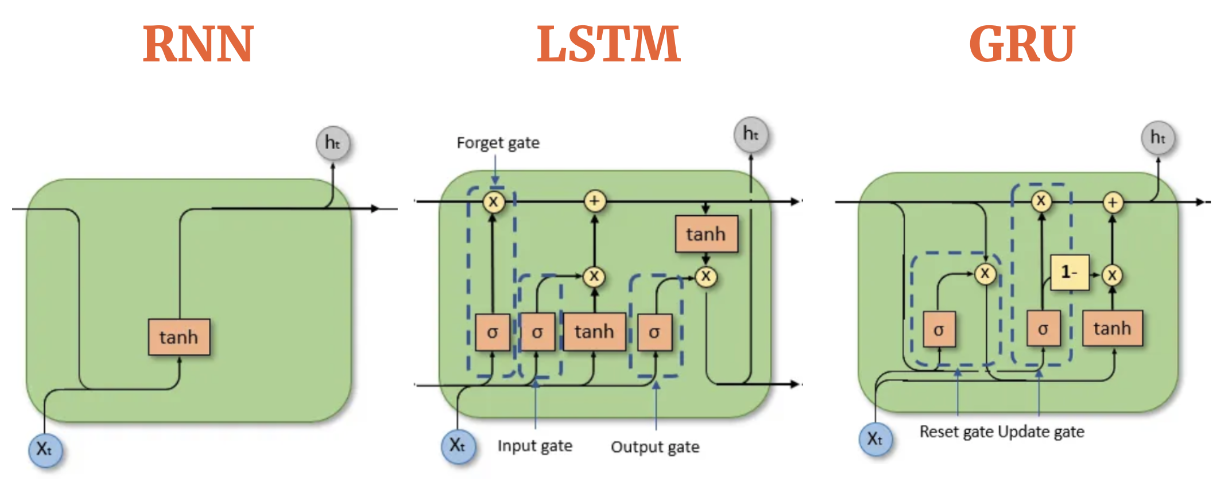
\includegraphics[width=0.6\textwidth]{figures/lstm-rnn-gru.png}
    \caption{Comparing different Sequence models: RNN, LSTM, and GRU. Source: Colah's blog. Compiled by AIML.com}\label{fig:lstm-rnn-gru}
\end{figure}

Early models integrated additional inputs such as environmental data and
semantic actions to enhance prediction accuracy. For
instance,~\citet{Alahi2016} proposed a Social-LSTM to model pedestrian
trajectories and interactions, further improving global context capture through
a social pooling module.

\subsection*{Transformer Models for Frame-Based Prediction}
Transformer model, introduced by~\citet{Vaswani2017}, has revolutionised
sequence modeling with its efficient and powerful network structure. For video
prediction, transformers leverage self-attention mechanisms to capture
long-range dependencies across frames. The~\citet{HowDoUGoWhere} study shows
how transformers can effectively learn mobility patterns from historical frame
sequences, achieving state-of-the-art performance in next-location prediction
tasks.

\subsection*{Frame-Based Approaches in Spatio-Temporal Prediction}

Video prediction, a critical task in spatio-temporal data analysis, involves
forecasting future frames based on past and current frames. This process
requires understanding both spatial and temporal dynamics within the data.

\subsubsection*{Convolutional LSTM (ConvLSTM)}

ConvLSTM integrates convolutional operations into LSTM units to better capture
spatial features in addition to temporal dependencies~\cite{ConvLSTM}. By
processing video data as sequences of frames, ConvLSTM effectively models the
spatio-temporal dependencies necessary for accurate video prediction. Each
frame serves as a spatial unit, and the sequence of frames provides temporal
context, allowing the model to predict future frames by learning from the
patterns in previous ones.

\subsubsection*{Cubic LSTM for Video Prediction}

The Cubic Long Short-Term Memory (CubicLSTM) unit, as proposed
by~\citet{CubicLSTMsVideoPrediction}, extends the capabilities of ConvLSTM by
separately processing spatial and temporal information through three branches:
temporal, spatial, and output. This approach mitigates the computational burden
and enhances prediction accuracy. Specifically:
\begin{itemize}
    \item The \textit{temporal branch} processes motion information by analysing the
          sequence of frames over time.
    \item The \textit{spatial branch} captures object information within individual
          frames.
    \item The \textit{output branch} combines temporal and spatial information to
          generate predicted future frames.
\end{itemize}
This separation of concerns allows the model to handle the complexities of video data more effectively, resulting in more accurate predictions of future frames.

\begin{figure}[H]
    \centering
    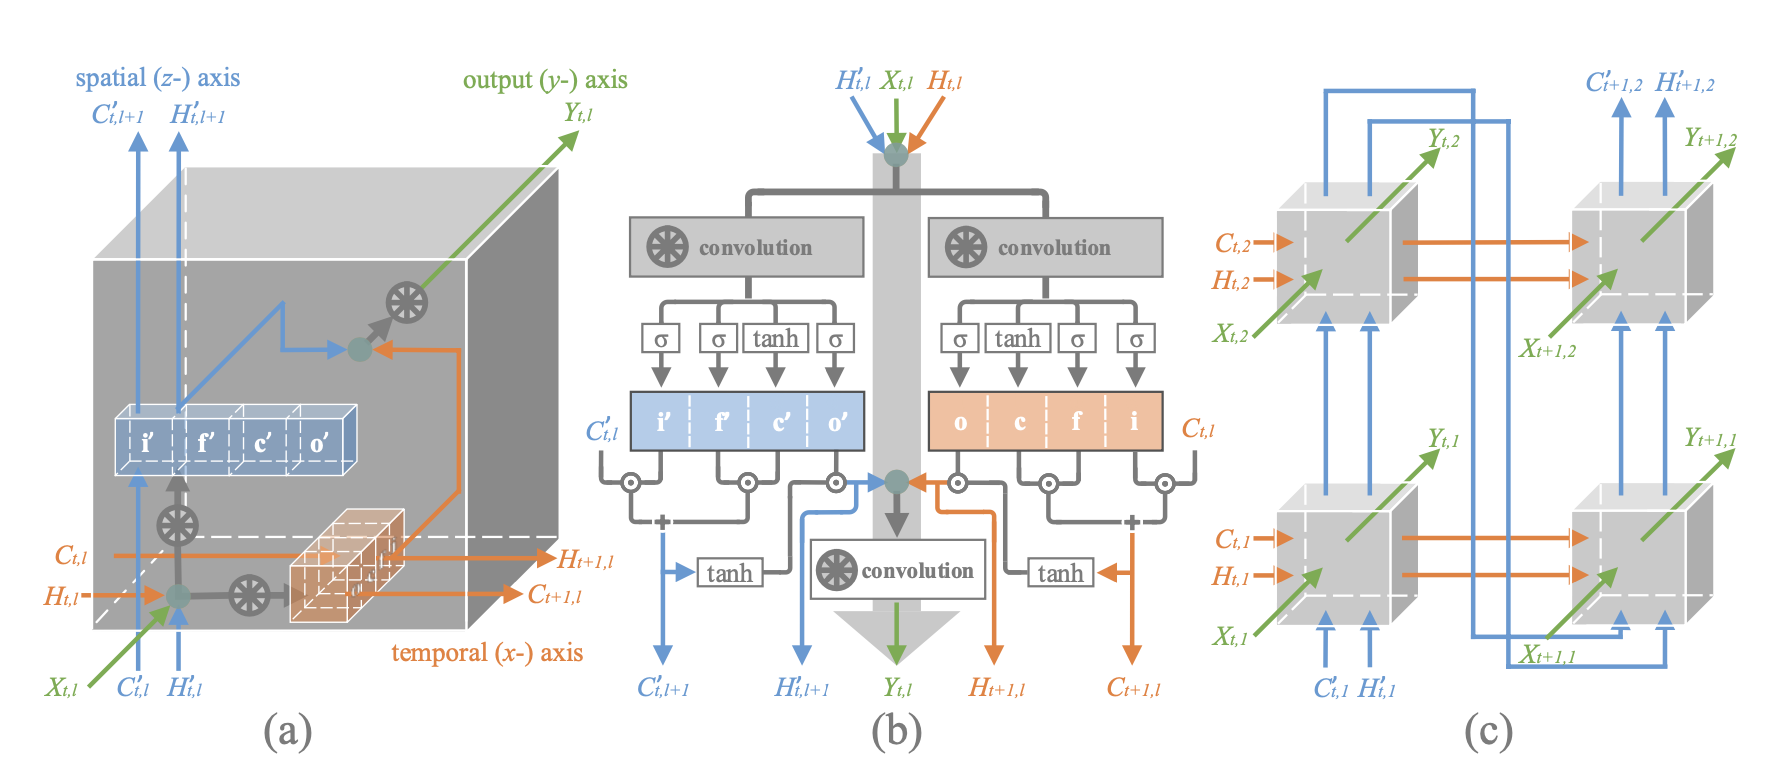
\includegraphics[width=1\textwidth]{figures/CubicLSTM.png}
    \caption{Cubic LSTM Architecture. (a) 3D structure of the CubicLSTM unit. (b) Topological diagram of the CubicLSTM unit. (c) Two-spatial-layer RNN composed of CubicLSTM units. The unit consists of three branches, a spatial (z-) branch for extracting and recognizing moving objects, a temporal (y-) branch for capturing and predicting motions, and an output (x-) branch for combining the first two branches to generate the predicted frames. Source:~\citet{CubicLSTMsVideoPrediction}}\label{fig:cubic-lstm}
\end{figure}

\subsubsection*{Unsupervised Video Forecasting with Flow Parsing}
\citet{UnsupervisedVideoForecastingFlowParsingMechanism} introduced an unsupervised video forecasting approach that incorporates a flow parsing mechanism. This model separates the motion and appearance learning processes:
\begin{itemize}
    \item The \textit{motion stream} predicts optical flow between frames to capture
          dynamic changes.
    \item The \textit{appearance stream} reconstructs frames to preserve spatial details.
\end{itemize}
By integrating these streams, the model can predict future frames with improved motion accuracy and appearance fidelity.

\begin{figure}[H]
    \centering
    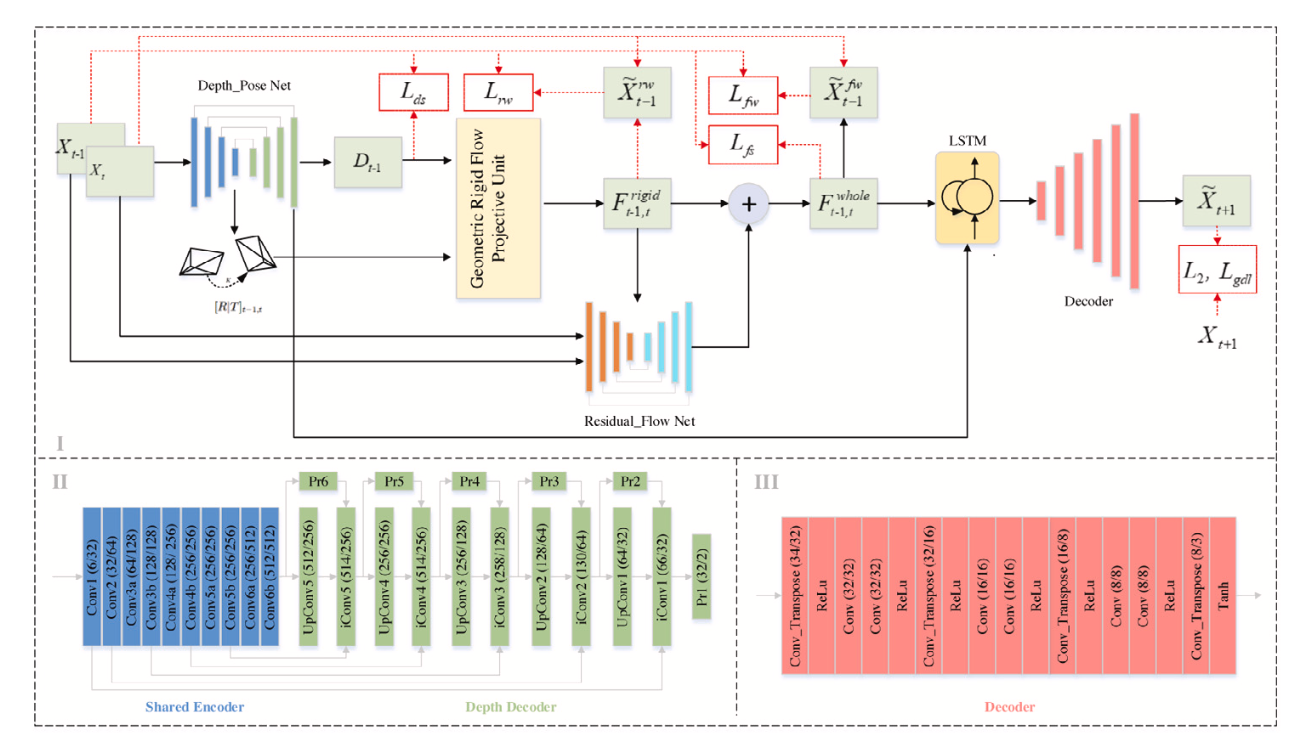
\includegraphics[width=1\textwidth]{figures/Unsupervised-Video-Forecasting.png}
    \caption{Model Architecture. Source:~\citet{UnsupervisedVideoForecastingFlowParsingMechanism}}\label{fig:unsupervised-video-forecasting-flow-parsing}
\end{figure}

\subsubsection*{Joint Optimization with Synthesis and Optical Flow Estimation}
\citet{VideoFramePredictionByJointOptimizationWithSynthesisAndOpticalFlowEstimation}
proposed a method that jointly optimizes frame synthesis and optical flow
estimation. Their approach leverages:
\begin{itemize}
    \item A \textit{frame synthesis network} to generate predicted frames.
    \item An \textit{optical flow estimation network} to capture motion dynamics between
          frames.
\end{itemize}
This joint optimization enhances the model's ability to produce accurate and visually coherent future frames.

\begin{figure}[H]
    \centering
    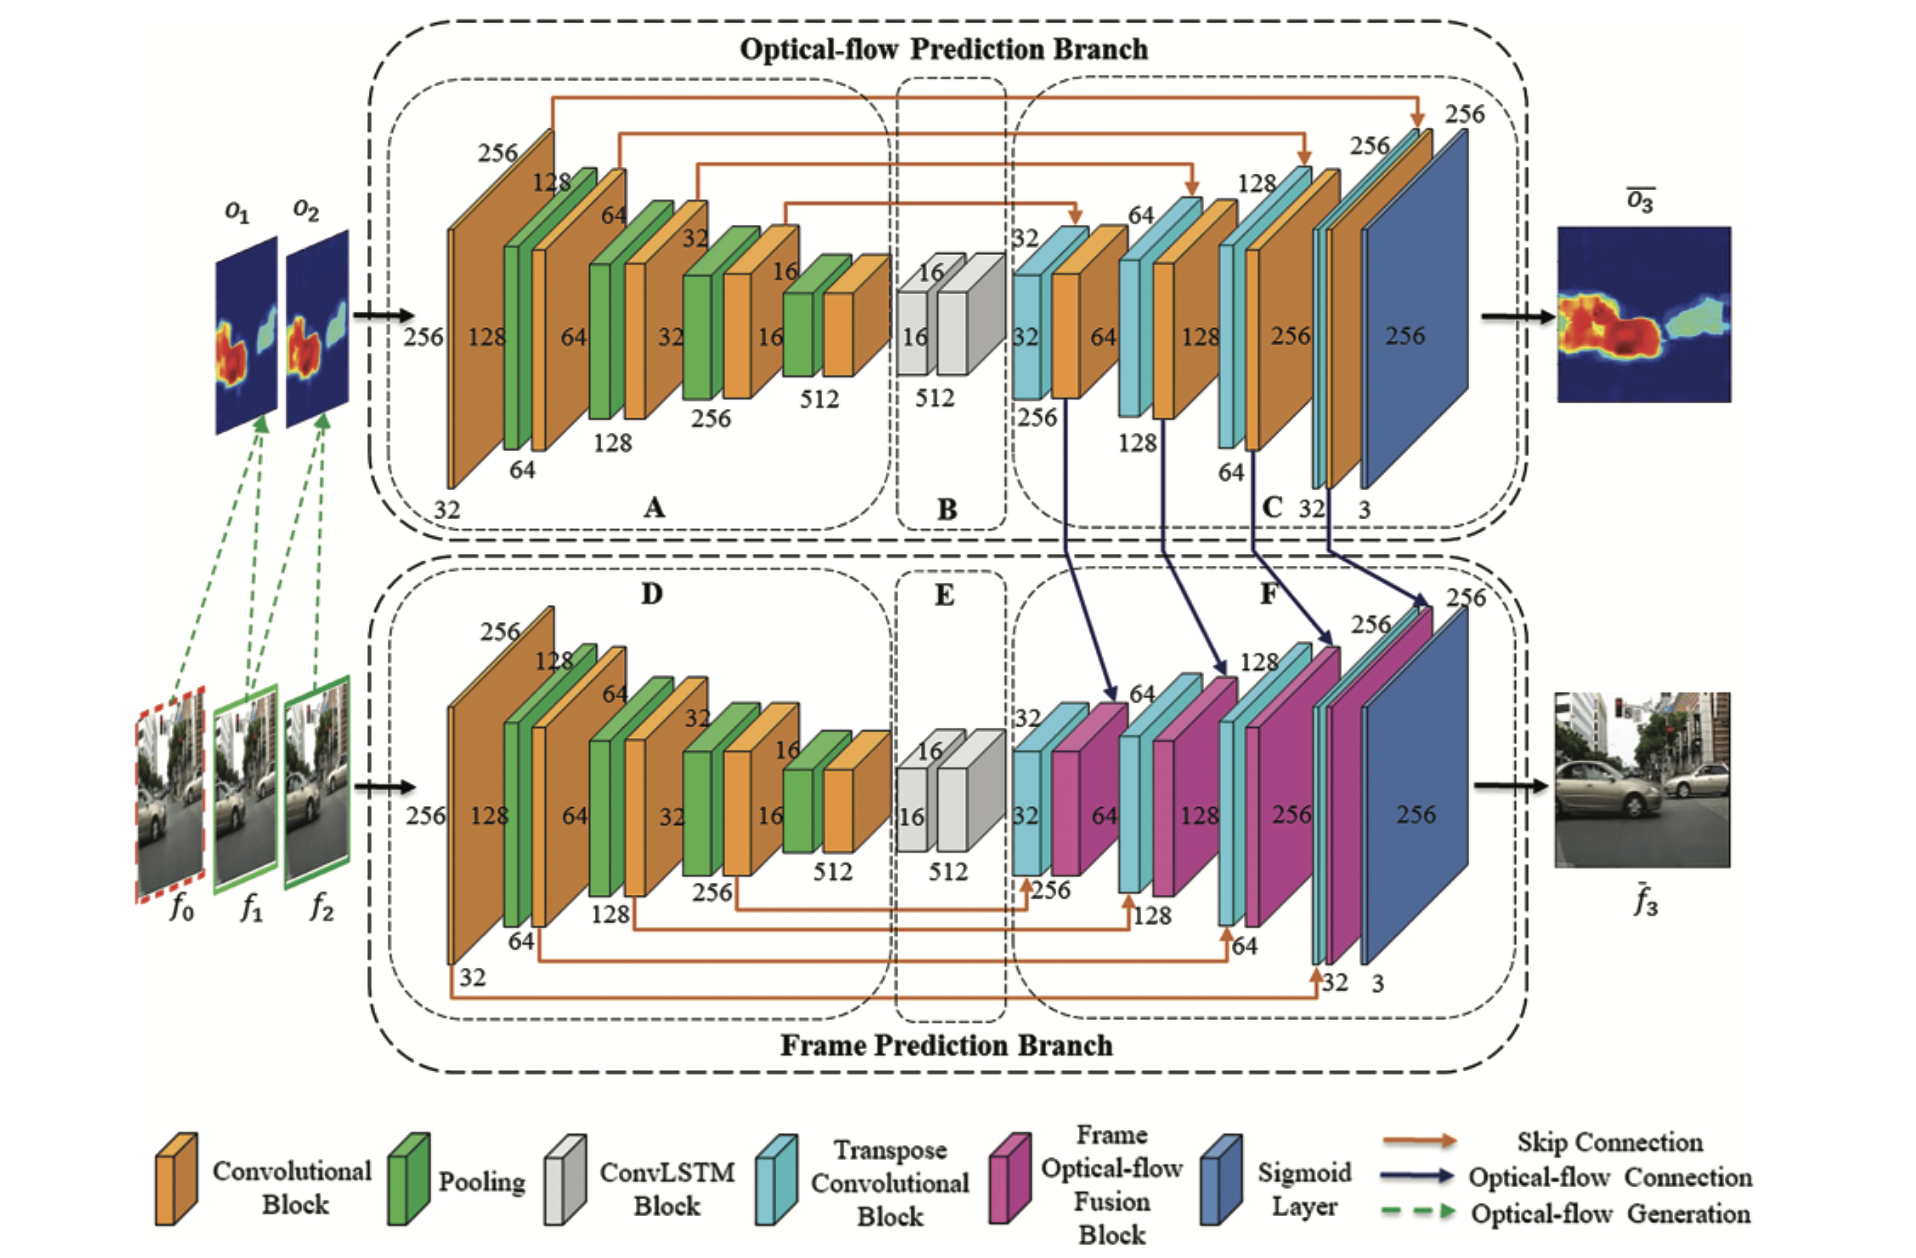
\includegraphics[width=0.8\textwidth]{figures/FPNet-OF.png}
    \caption{FPNet-OF model architecture. Source:~\citet{VideoFramePredictionByJointOptimizationWithSynthesisAndOpticalFlowEstimation}}\label{fig:joint-optimization-synthesis-optical-flow}
\end{figure}

\subsubsection*{Fusion-GRU}
\citet{FusionGRU} developed the Fusion-Gated Recurrent
Unit (Fusion-GRU) model to predict the future bounding boxes of traffic agents
in risky driving scenarios. This model leverages multiple sources of
information, including location-scale data, monocular depth information, and
optical flow data, to capture complex interactions among information cues and
transform them into hidden representations. The Fusion-GRU model uses an
intermediary estimator and self-attention aggregation layer to enhance
sequential dependencies for long-term predictions, demonstrating superior
performance in challenging driving scenarios.

\begin{figure}[H]
    \centering
    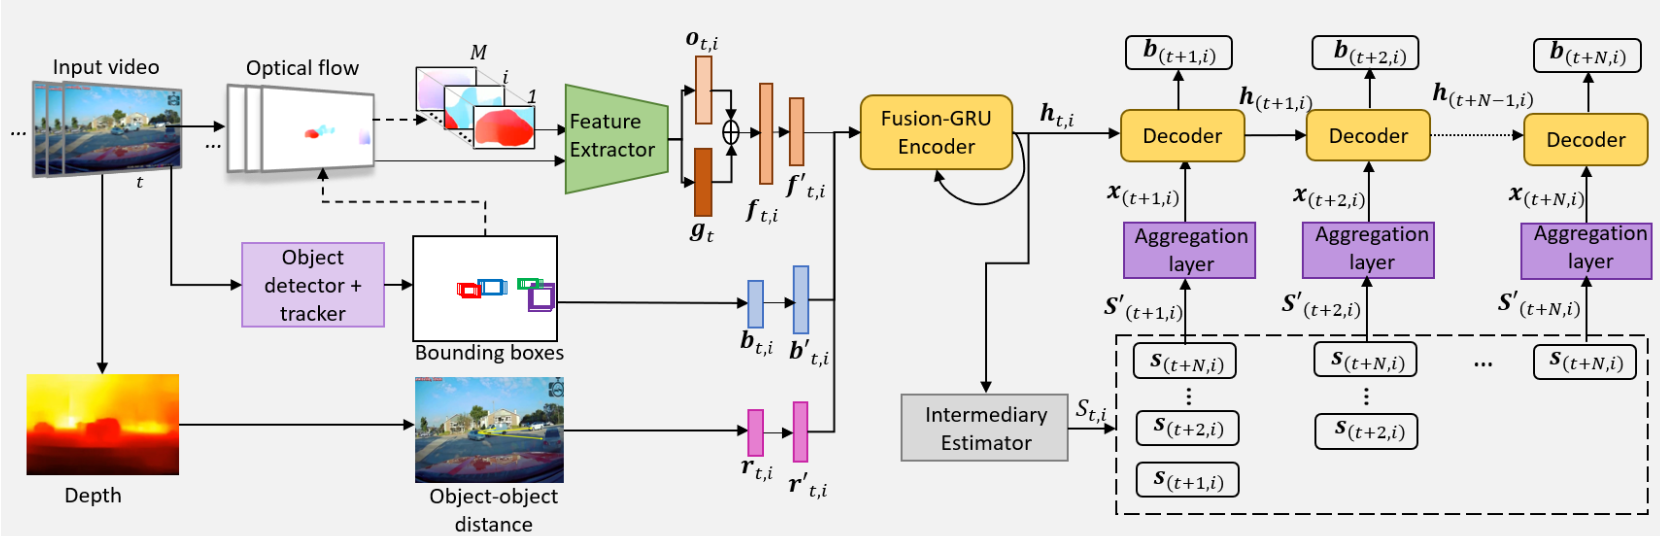
\includegraphics[width=1\textwidth]{figures/FusionGRU.png}
    \caption{Fusion-GRU model architecture. Source:~\citet{FusionGRU}}\label{fig:fusion-gru}
\end{figure}

\subsubsection*{Dual-Branch Spatial-Temporal Learning Network}

Huang and Guan~\cite{DualBranchSpatialTemporalLearningNetworkVideoPrediction}
proposed a dual-branch video prediction network that aims to generate
high-quality future frames by simultaneously capturing complex motion patterns
and preserving appearance information. Their network includes two distinct
units:
\begin{itemize}
    \item The \textit{motion prediction unit (MPU)} focuses on inter-frame motion and
          intra-frame appearance by using depth and multiple-scale convolutions, along
          with temporal attention mechanisms to enhance feature interactions over time.
    \item The \textit{spatial prediction unit (SPU)} concentrates on spatial information,
          ensuring appearance consistency across video frames by capturing various
          appearance features.
\end{itemize}
This dual-branch approach addresses the limitations of relying on external information or complex state transition units, resulting in better visual quality and fewer blurry artifacts in predicted frames.

\begin{figure}[H]
    \centering
    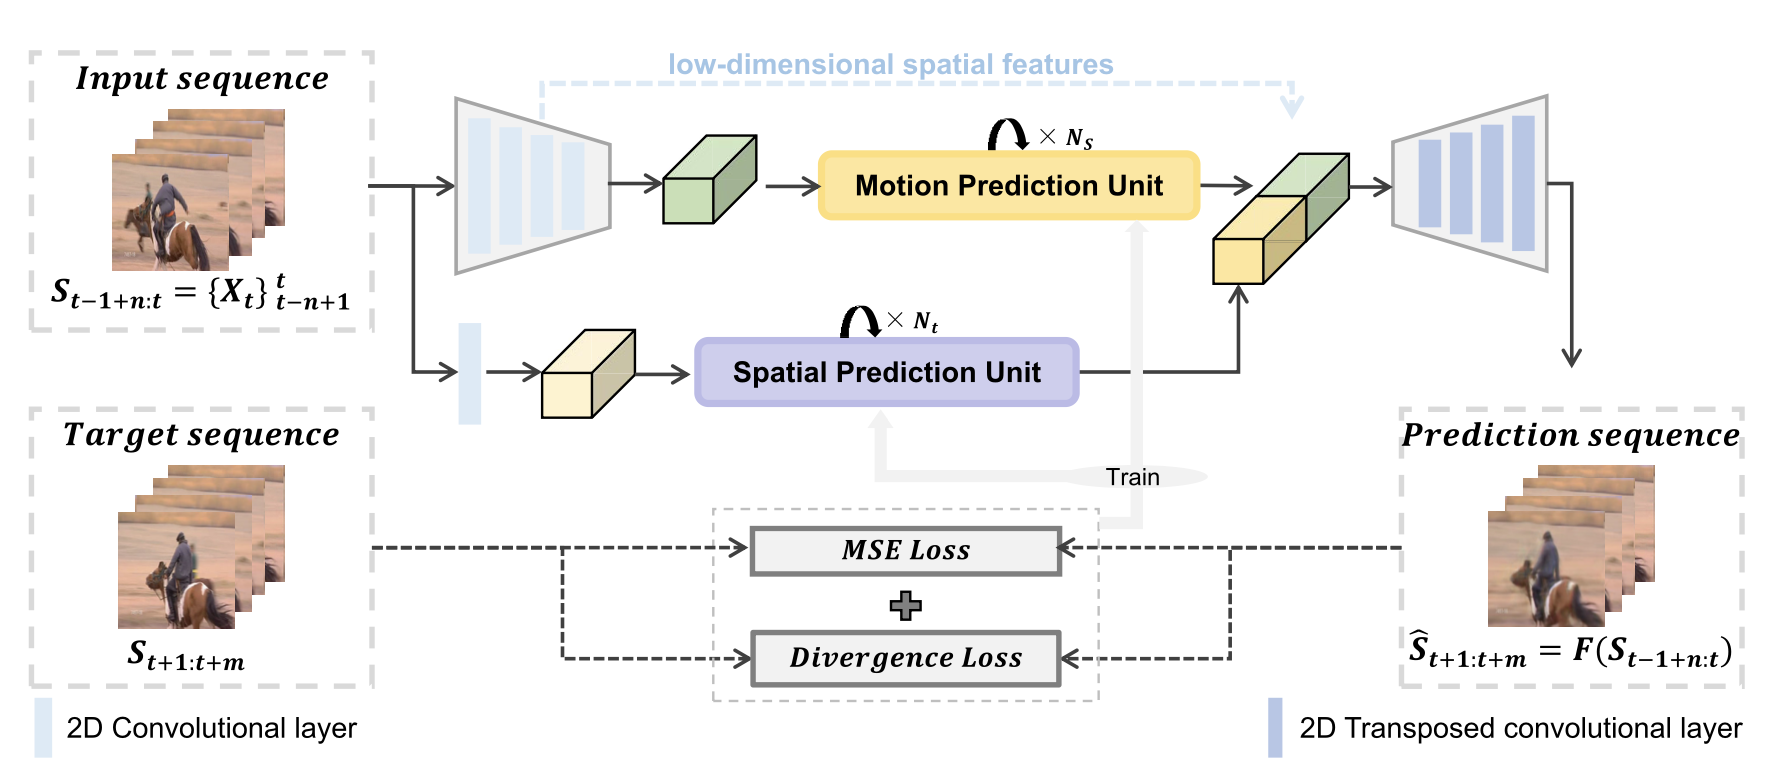
\includegraphics[width=0.7\textwidth]{figures/dual-branch-architecture.png}
    \caption{Dual-Branch Spatial-Temporal Learning Network. Source:~\citet{DualBranchSpatialTemporalLearningNetworkVideoPrediction}}\label{fig:dual-branch-spatial-temporal-learning-network}
\end{figure}

\begin{figure}[H]
    \centering
    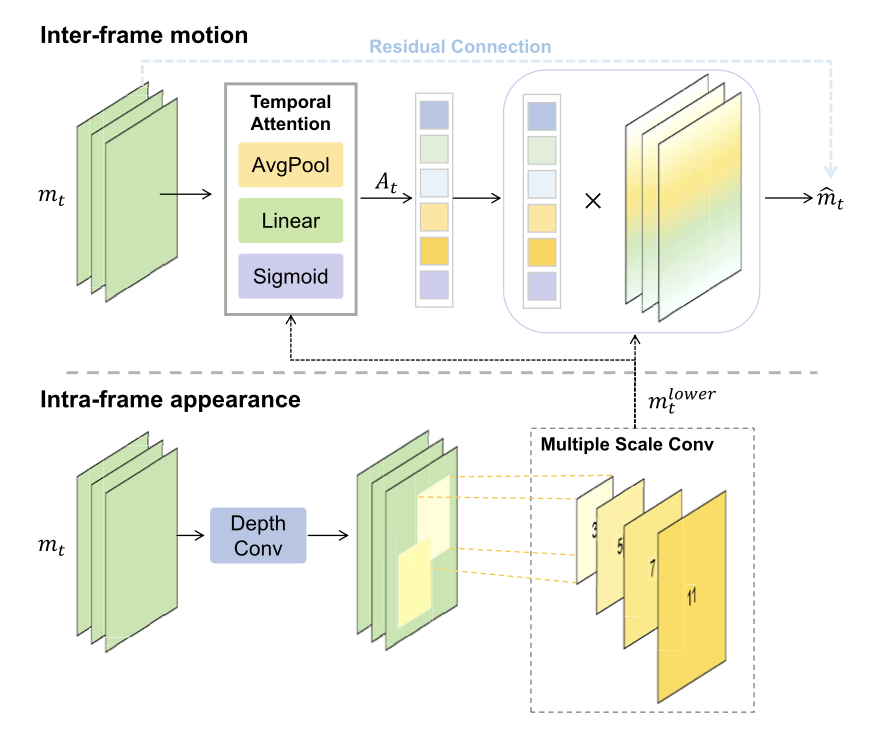
\includegraphics[width=0.5\textwidth]{figures/dual-branch-inter-intra-frames.png}
    \caption{Dual-Branch Spatial-Temporal Learning Network. Source:~\citet{SurveyDLOD}}\label{fig:dual-branch-inter-intra-frames}
\end{figure}

\subsection*{Applications and Case Studies}

In various applications, the frame-based approach to spatio-temporal prediction
has proven highly effective:

\subsubsection*{Moving-MNIST Dataset}

The Moving-MNIST dataset consists of sequences of moving handwritten digits.
Each sequence includes a series of frames, and the goal is to predict future
frames based on the observed ones. This dataset contains 10000 videos, each
consisting of 20 frames~\cite{DBLP:journals/corr/SrivastavaMS15}. The
CubicLSTM-based CubicRNN demonstrated superior accuracy compared to traditional
ConvLSTM models, showcasing its ability to capture both motion and spatial
features effectively~\cite{ CubicLSTMsVideoPrediction}.

\begin{figure}[H]
    \centering
    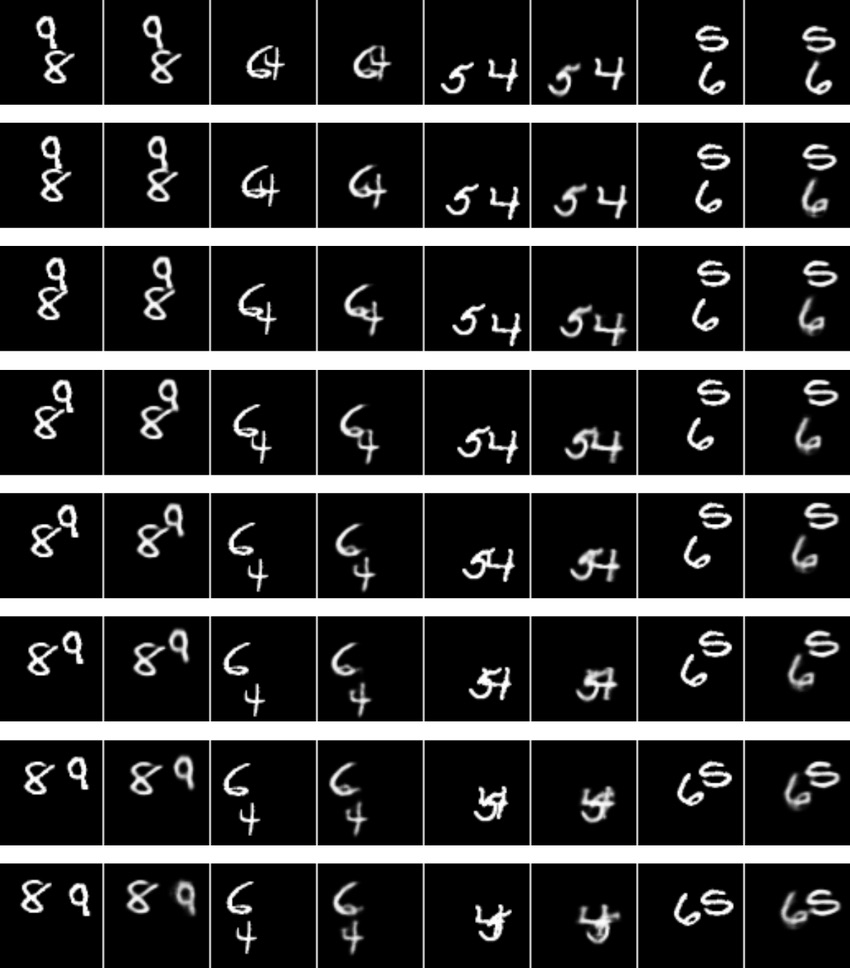
\includegraphics[width=0.3\textwidth]{figures/2-digit-Moving-MNIST-data-Fig-5-3-digit-Moving-MNIST-data.jpeg}
    \caption{2-digit Moving MNIST data by~\citet{DBLP:journals/corr/SrivastavaMS15}}\label{fig:moving-mnist}
\end{figure}

\subsubsection*{Robotic Pushing Dataset}

This dataset involves sequences of robotic arms pushing objects, with each
frame representing a step in the sequence. The dataset contains 3456 training
images with labels and 1024 validation images with
labels~\cite{DBLP:journals/corr/FinnGL16}. The CubicLSTM model, combined with
convolutional dynamic neural advection (CDNA) models, achieved higher accuracy
and generated clearer frames compared to ConvLSTM and CNN-based models. This
application highlights the importance of accurately predicting future frames to
understand and anticipate the movements of robotic
systems~\cite{CubicLSTMsVideoPrediction}.

\begin{figure}[H]
    \centering
    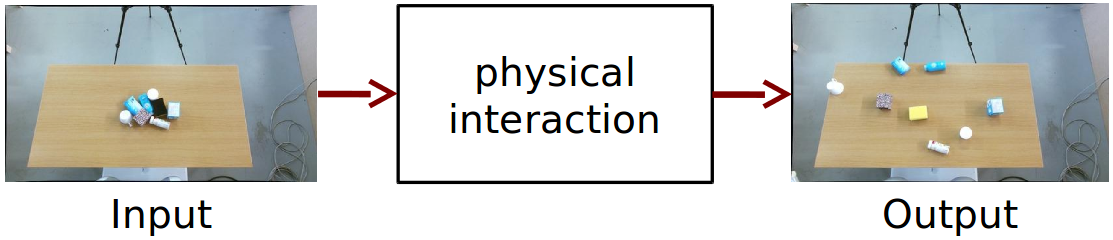
\includegraphics[width=0.5\textwidth]{figures/robotpush.png}
    \caption{Robotic Pushing Dataset. Source:~\citet{DBLP:journals/corr/EitelHB17}}\label{fig:robotic-pushing-dataset}
\end{figure}

\subsubsection*{KTH Action Dataset}

The KTH Action dataset features videos of people performing various actions,
with each video divided into frames. The dataset contains 2391
sequences~\cite{KTH}. The CubicLSTM model provided more accurate and visually
consistent predictions of future frames compared to other state-of-the-art
models like DrNet and MCnet. This demonstrates the model's effectiveness in
understanding and predicting human actions over
time~\cite{CubicLSTMsVideoPrediction}.

\begin{figure}[H]
    \centering
    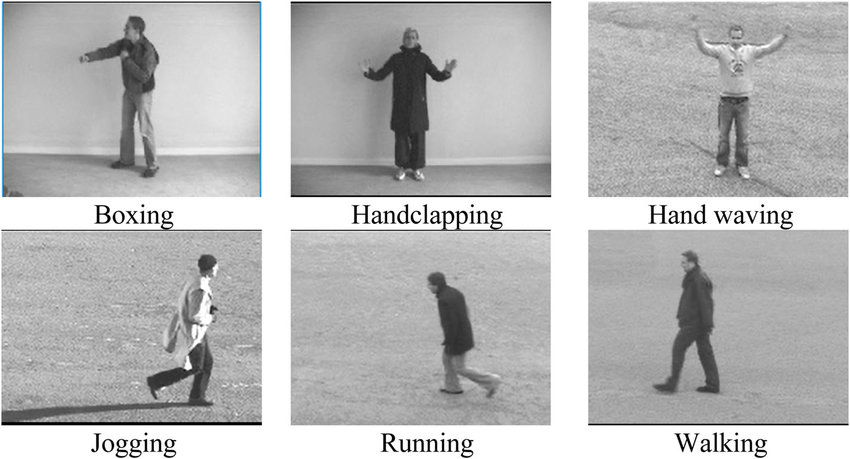
\includegraphics[width=0.5\textwidth]{figures/KTH-dataset.png}
    \caption{KTH Action Dataset. Source:~\citet{KTH}}\label{fig:kth-action-dataset}
\end{figure}

\subsubsection*{UCF Sports Dataset}

The UCF Sports dataset consists of a collection of footage collected from
various sports that are typically shown on television channels such as the BBC
and ESPN.\@ It comprises a total of 150 sequences~\cite{UCFSport}. Huang and
Guan's dual-branch network was tested on the UCF Sports dataset, which includes
complex motion patterns and large movements. Their method outperformed other
state-of-the-art methods in terms of visual quality and motion accuracy, as
evidenced by superior metrics such as PSNR, SSIM, and LPIPS. The results
validate the network's ability to handle intricate video prediction tasks
without relying on additional information~\cite{
    DualBranchSpatialTemporalLearningNetworkVideoPrediction}.

\begin{figure}[H]
    \centering
    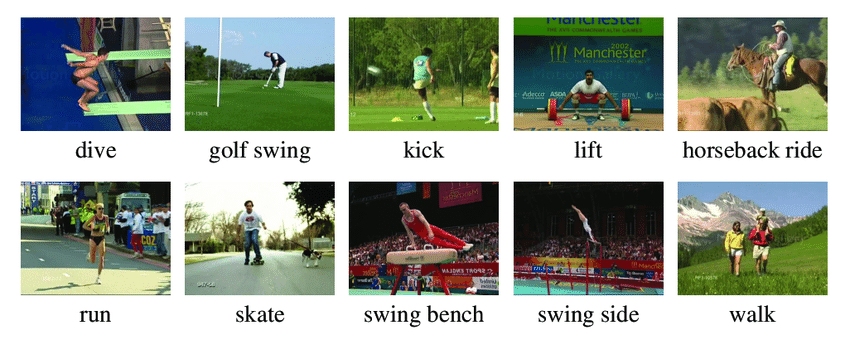
\includegraphics[width=0.6\textwidth]{figures/ucf-sport-dataset.png}
    \caption{UCF Sports Dataset. Source:~\citet{UCFSport}}\label{fig:ucf-sports-dataset}
\end{figure}

%%%%%%%%%%%%%%%%%%%%%%%%%%%%%%%%%%%%%%%%%%%%%%%%%%%%%%%%%%%%%%%%%%%%%%%%%%%%%%%
%%%%%%%%%%%%%%%%%%%%%%%%%%%%%%%%% METHODOLOGY %%%%%%%%%%%%%%%%%%%%%%%%%%%%%%%%%
\chapter{Methodology}\label{chap:methodology}
\section{Dataset Configuration}
\subsection{Provided Dataset Description}
The `Indoor Hangar Fueling Port Detection and Tracking Dataset' (HARD) is an
integral part of Phase-1 of the ONEHeart project, funded by UKRI. The ONEHeart
project aims to develop an automated aircraft refuelling system based on
computer vision and robotics technology. This dataset can be utilised for
various purposes, including but not limited to refueling port detection,
fueling port tracking, camera pose estimation, and visual image processing. It
is provided under the terms of the UKRI funding agreement. Unauthorised use,
distribution, or reproduction is prohibited.

The HARD dataset consists of 21 video sequences captured in an indoor hangar at
the Aerospace Integration Research Centre (AIRC). The videos were recorded
using an Intel® ${\text{RealSense}}^{\text{TM}}$ D435~\cite{IntelRealSense}
(Shown in Figure~\ref{fig:intel-realsense-d435}), which provides depth
information in addition to RGB data. The target area for detection and tracking
is near the refueling port of an Airbus A320 wing. The videos were recorded
under different lighting conditions, including indoor artificial lighting and
natural daylight, to simulate real-world scenarios.

\begin{figure}[H]
    \centering
    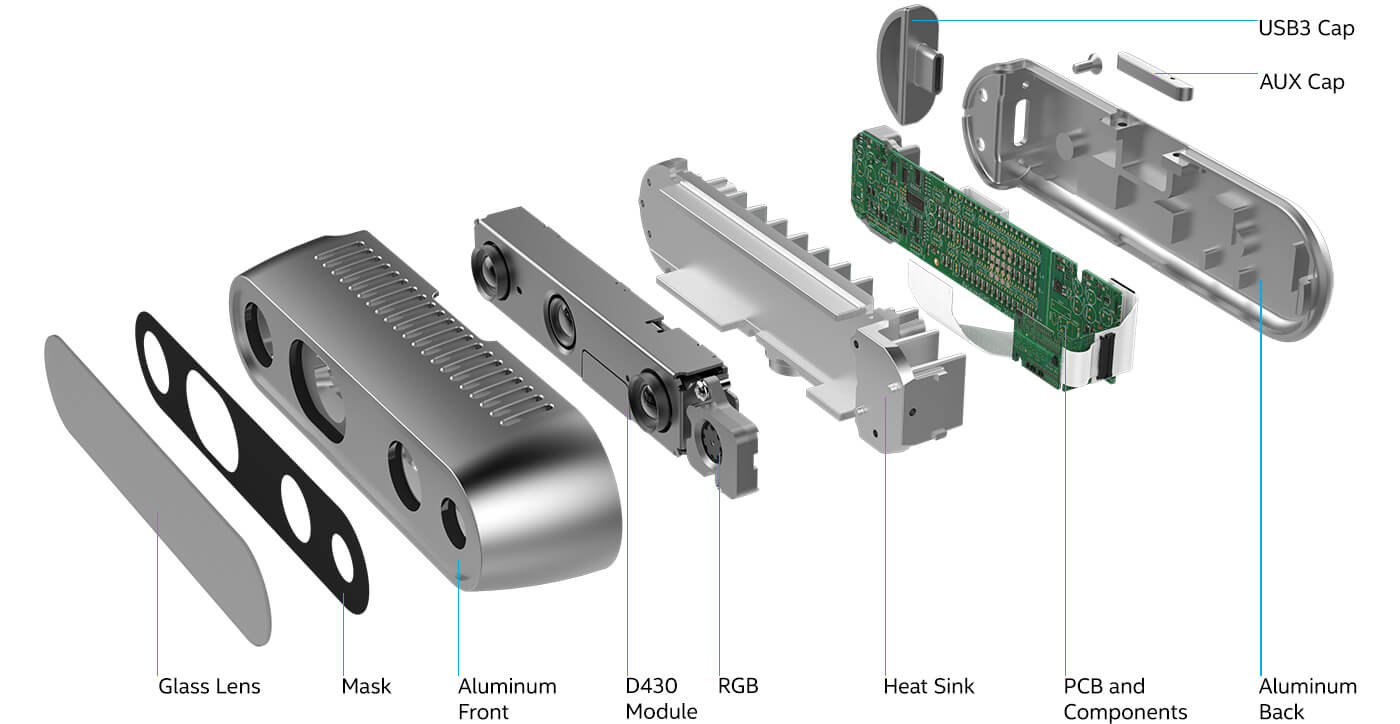
\includegraphics[width=0.7\textwidth]{figures/depth-camera-d435_details.jpg}
    \caption{Intel® ${\text{RealSense}}^{\text{TM}}$ D435 Depth Camera. Source: Intel}\label{fig:intel-realsense-d435}
\end{figure}

There are three states of the refueling port in the dataset:
\begin{itemize}
    \item \textbf{CLOSED}: The refueling port is closed.
    \item \textbf{OPEN}: The refueling port is open.
    \item \textbf{SEMI-OPEN}: The refueling port is partially open.
\end{itemize}

\subsection{Data Annotation}
The HARD dataset provided for this project was not fully annotated. Therefore,
the first step in the data preparation process was to annotate the dataset.
This annotation process was crucial to enable the training of machine learning
models for accurate refueling port detection and tracking.

The annotation process involved several steps:
\begin{enumerate}
    \item \textbf{Initial Manual Annotation}: Initially, 100 frames from each video sequence were manually annotated. This involved labeling the refueling port in each frame, which required identifying and marking the exact location of the refueling port using bounding boxes. This was done using the Label Studio tool, a powerful annotation platform that allows users to create and manage annotations in images and videos.
    \item \textbf{Tool Used - Label Studio}: Label Studio was chosen for its flexibility and ease of use. It supports various annotation formats and integrates well with machine learning workflows. Users can draw bounding boxes around objects of interest, in this case, the refueling port, to create labeled datasets.
    \item \textbf{Preliminary Dataset Creation}: The initial manual annotations created a preliminary dataset. This dataset was used to train a YOLOv10 (You Only Look Once, version 10) model for refueling port detection.
    \item \textbf{Model Training}: The annotated dataset was used to train the YOLOv10 model. The model learned to detect the refueling port from the annotated images, improving its accuracy with each training iteration.
    \item \textbf{Automated Annotation}: After training the YOLOv10 model, it was implemented as a backend service for Label Studio. This was deployed as a Docker container, allowing the model to be used for automated annotation of the remaining images in the dataset. The model predicted the location of the refueling port in new frames, and these predictions were used to annotate the rest of the dataset automatically.
    \item \textbf{Review and Quality Control}: Each automatically generated annotation was reviewed manually to ensure accuracy. This review process involved verifying the location of the refueling port in each frame and making necessary corrections to the annotations. This thorough quality control ensured that the entire dataset was consistently and accurately labeled.
\end{enumerate}

This comprehensive annotation process ensured that the entire dataset was
accurately labeled, providing a robust foundation for training machine learning
models aimed at refueling port detection and tracking. The combination of
manual and automated annotation techniques maximised efficiency while
maintaining high annotation quality.

\subsection{Summary of Available Videos}
Each video was assigned to a specific dataset (train, val, and test), with an
approximate split of 70\% for training, 15\% for validation, and 15\% for
testing. The following table presents the available videos in the dataset along
with the number of frames for each video and their assignment:

\begin{table}[H]
    \centering
    \begin{tabular}{@{}cccc@{}}
        \toprule
        \textbf{Type}      & \textbf{Video Name}                           & \textbf{Number of Frames} & \textbf{Assignment} \\ \midrule
        \textbf{Closed}    & \textbf{video\_lab\_platform\_1}              & \textbf{624}              & \textbf{train}      \\
        Closed             & video\_lab\_platform\_2                       & 639                       & train               \\
        Closed             & video\_lab\_platform\_5                       & 398                       & train               \\
        Closed             & video\_lab\_platform\_7                       & 412                       & train               \\
        Closed             & video\_lab\_platform\_8                       & 470                       & train               \\
        Closed             & video\_lab\_platform\_9                       & 373                       & train               \\
        Closed             & video\_lab\_manual\_1                         & 746                       & train               \\
        Closed             & video\_lab\_platform\_3                       & 569                       & val                 \\
        Closed             & video\_lab\_platform\_4                       & 247                       & val                 \\
        Closed             & video\_lab\_platform\_6                       & 303                       & test                \\
        Closed             & test\_outdoor1                                & 499                       & test                \\
        \textbf{Open}      & \textbf{video\_lab\_open\_1\_\_\_\_\_\_1}     & \textbf{497}              & \textbf{train}      \\
        Open               & video\_lab\_open\_1\_\_\_\_\_\_2              & 602                       & train               \\
        Open               & video\_lab\_open\_1\_\_\_\_\_\_3              & 313                       & train               \\
        Open               & video\_lab\_open\_1\_\_\_\_\_\_4              & 310                       & train               \\
        Open               & test\_indoor2                                 & 310                       & val                 \\
        Open               & test\_indoor1                                 & 314                       & test                \\
        \textbf{Semi-Open} & \textbf{video\_lab\_semiopen\_1\_\_\_\_\_\_1} & \textbf{739}              & \textbf{train}      \\
        Semi-Open          & video\_lab\_semiopen\_1\_\_\_\_\_\_2          & 439                       & train               \\
        Semi-Open          & video\_lab\_semiopen\_1\_\_\_\_\_\_4          & 372                       & val                 \\ 
        Semi-Open          & video\_lab\_semiopen\_1\_\_\_\_\_\_3          & 383                       & test                \\ \bottomrule
    \end{tabular}
    \caption{\centering Summary of available videos in the HARD dataset with their assignment.}
    \label{tab:video_summary}
\end{table}

\subsection{Initial Data Distribution}
Before balancing the data, the distribution of video frames across the
different datasets (train, validation, and test) for each state of the fueling
port (CLOSED, OPEN, and SEMI-OPEN) was as follows:
\begin{table}[H]
    \centering
    \begin{tabular}{@{}ccccc@{}}
        \toprule
        \textbf{Type}      & \textbf{Total Frames} & \textbf{Train} & \textbf{Test} & \textbf{Validation} \\ \midrule
        \textbf{CLOSED}    & 5280                  & 3662 (69.36\%) & 802 (15.19\%) & 816 (15.45\%)       \\ 
        \textbf{OPEN}      & 2346                  & 1722 (73.40\%) & 314 (13.38\%) & 310 (13.21\%)       \\ 
        \textbf{SEMI-OPEN} & 1933                  & 1178 (60.94\%) & 383 (19.81\%) & 372 (19.24\%)       \\ \bottomrule
    \end{tabular}
    \caption{\centering Distribution of frames across train, test, and validation sets for each state in the HARD dataset before balancing.}
    \label{tab:frame_distribution}
\end{table}

As shown in~\ref{tab:frame_distribution}, the dataset initially had an
imbalance in the number of frames for each state. For instance, the CLOSED
state had significantly more frames compared to the OPEN and SEMI-OPEN states.
This imbalance could lead to biased training and inaccurate model performance,
as the model might become overly familiar with the more prevalent CLOSED state
and underperform on the less represented states.

\subsection{Balanced Data Distribution}
To address this issue, a balancing strategy was employed to create a more
uniform dataset. The steps taken were as follows:
\begin{enumerate}
    \item \textbf{Shuffling and Subsetting}: Each state (CLOSED, OPEN, and SEMI-OPEN) subset was shuffled, and only the minimum number of frames from each state was kept. This step ensured that the number of frames for each state was equal, avoiding bias toward any particular state.
    \item \textbf{Merging Subsets}: The subsets were merged to create three balanced datasets: Training, Validation, and Test, each with an equal number of frames for each state.
    \item \textbf{Final Shuffling and Resizing}: Each balanced dataset was shuffled again and resized to maintain the required split ratio of 70\% for training, 15\% for validation, and 15\% for testing.
\end{enumerate}

The balanced dataset will be used for training and evaluating the object
detection model, while the full dataset will be utilised for sequence model
training and framework evaluation.

The resulting distribution of frames across the train, test, and validation
sets for each state after balancing is as follows:
\begin{table}[H]
    \centering
    \begin{tabular}{@{}cc@{}}
        \toprule
        \textbf{Dataset} & \textbf{Total Frames} \\ \midrule
        \textbf{Train}   & 3534 (69.57\%)        \\ 
        \textbf{Test}    & 773  (15.22\%)        \\ 
        \textbf{Val}     & 773  (15.22\%)        \\ \bottomrule
    \end{tabular}
    \caption{\centering Distribution of frames across train, test, and validation sets for each state in the HARD dataset after balancing.}
    \label{tab:balanced_frame_distribution}
\end{table}

The primary reason for balancing the dataset is to ensure that the object
detection model is equally trained on all states of the refueling port. An
imbalanced dataset could cause the model to perform well on the more common
states (like CLOSED) while underperforming on the less common states (like OPEN
and SEMI-OPEN). By balancing the dataset:

\begin{itemize}
    \item \textbf{Improved Generalization}: The model will have an equal opportunity to learn from all states, improving its generalization and robustness.
    \item \textbf{Avoiding Bias}: Equal representation of each state prevents the model from becoming biased towards any particular state.
    \item \textbf{Consistent Performance}: This strategy ensures consistent performance across all states, which is critical for the reliable operation of the automated refueling system.
\end{itemize}

\subsection{Example Images from the Dataset}
The following figures show annotated examples of the refueling port in
different states:
\begin{figure}[H]
    \centering
    \includegraphics[width=0.45\textwidth]{figures/grid\_closed\_images.png}
    \caption{Annotated images of the refueling port in the CLOSED state.}~\label{fig:grid-closed-images}
\end{figure}

\begin{figure}[H]
    \centering
    \includegraphics[width=0.45\textwidth]{figures/grid\_open\_images.png}
    \caption{Annotated images of the refueling port in the OPEN state.}~\label{fig:grid-open-images}
\end{figure}

\begin{figure}[H]
    \centering
    \includegraphics[width=0.45\textwidth]{figures/grid\_semiopen\_images.png}
    \caption{Annotated images of the refueling port in the SEMI-OPEN state.}~\label{fig:grid-semi-open-images}
\end{figure}

\subsection{Sequence Model Data Preparation}
\begin{figure}[H]
    \centering
    \begin{subfigure}[t]{0.6\textwidth}
        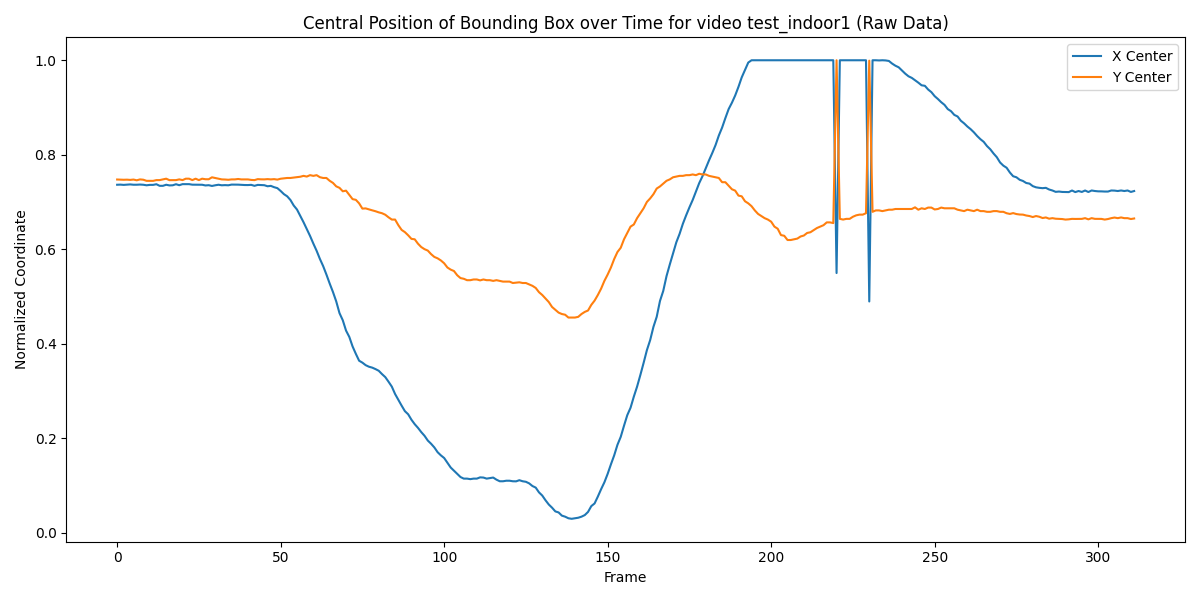
\includegraphics[width=\textwidth]{figures/bbox_metrics/test_indoor1 (Raw Data)_central_position.png}
        \caption{Central position of the refueling port over time.}
        \label{fig:central-position-test-indoor1}
    \end{subfigure}
    \hfill
    \begin{subfigure}[t]{0.6\textwidth}
        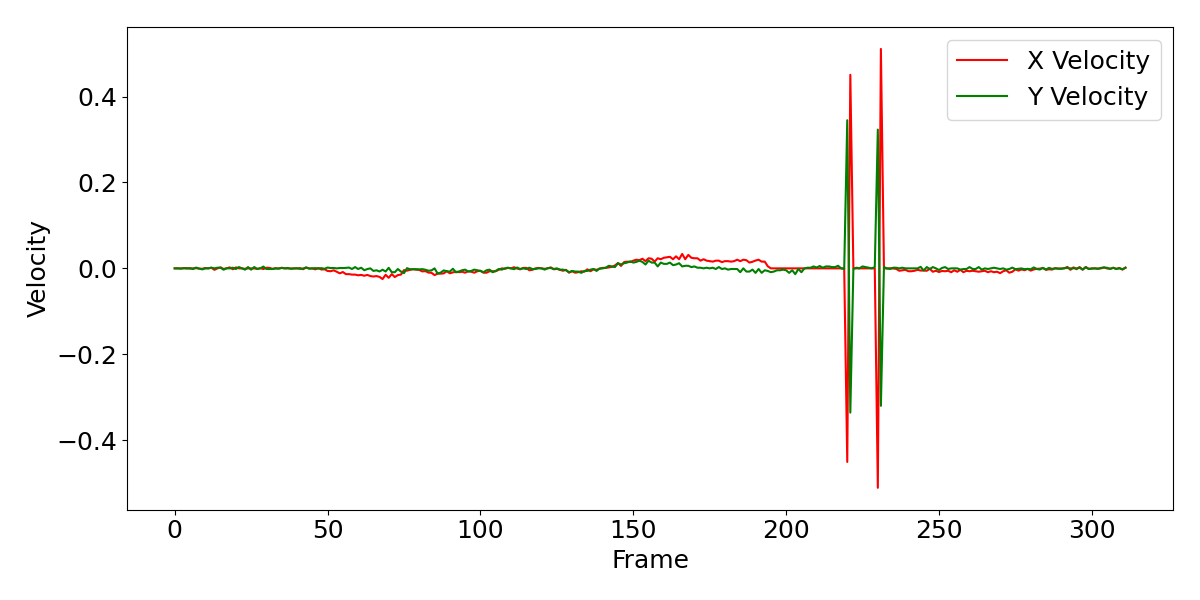
\includegraphics[width=\textwidth]{figures/bbox_metrics/test_indoor1 (Raw Data)_velocity.png}
        \caption{Velocity of the refueling port over time.}
        \label{fig:velocity-test-indoor1}
    \end{subfigure}
    \vfill
    \begin{subfigure}[t]{0.6\textwidth}
        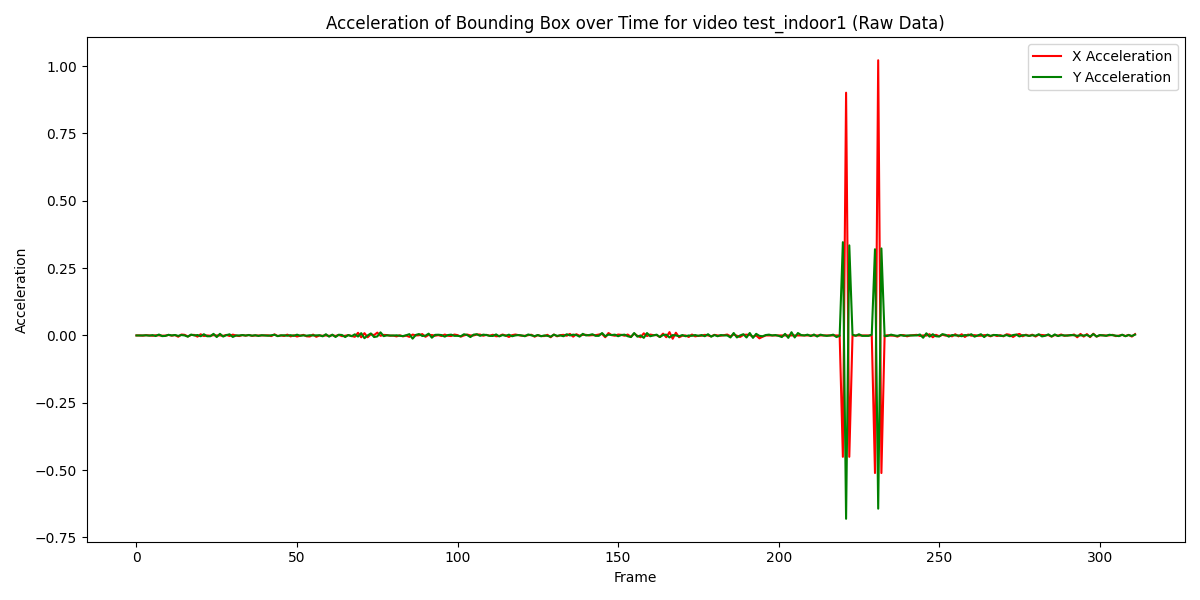
\includegraphics[width=\textwidth]{figures/bbox_metrics/test_indoor1 (Raw Data)_acceleration.png}
        \caption{Acceleration of the refueling port over time.}
        \label{fig:acceleration-test-indoor1}
    \end{subfigure}
    \hfill
    \begin{subfigure}[t]{0.6\textwidth}
        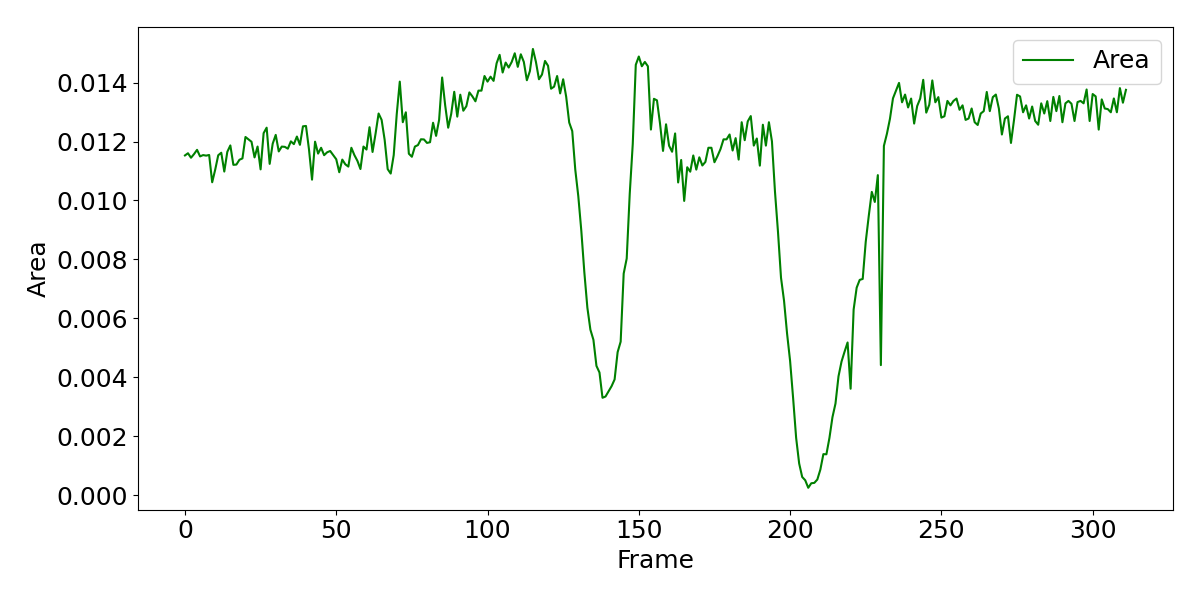
\includegraphics[width=\textwidth]{figures/bbox_metrics/test_indoor1 (Raw Data)_area.png}
        \caption{Area of the refueling port over time.}
        \label{fig:size-test-indoor1}
    \end{subfigure}
    \caption{Temporal analysis of different metrics for the refueling port in the \textit{test\_indoor1} video. The metrics include (a) central position, (b) velocity, (c) acceleration, and (d) area, providing a comprehensive overview of the object's dynamics over time.}
    \label{fig:bbox-metrics-test-indoor1}
\end{figure}

\begin{figure}[H]
    \centering
    \begin{subfigure}[t]{0.6\textwidth}
        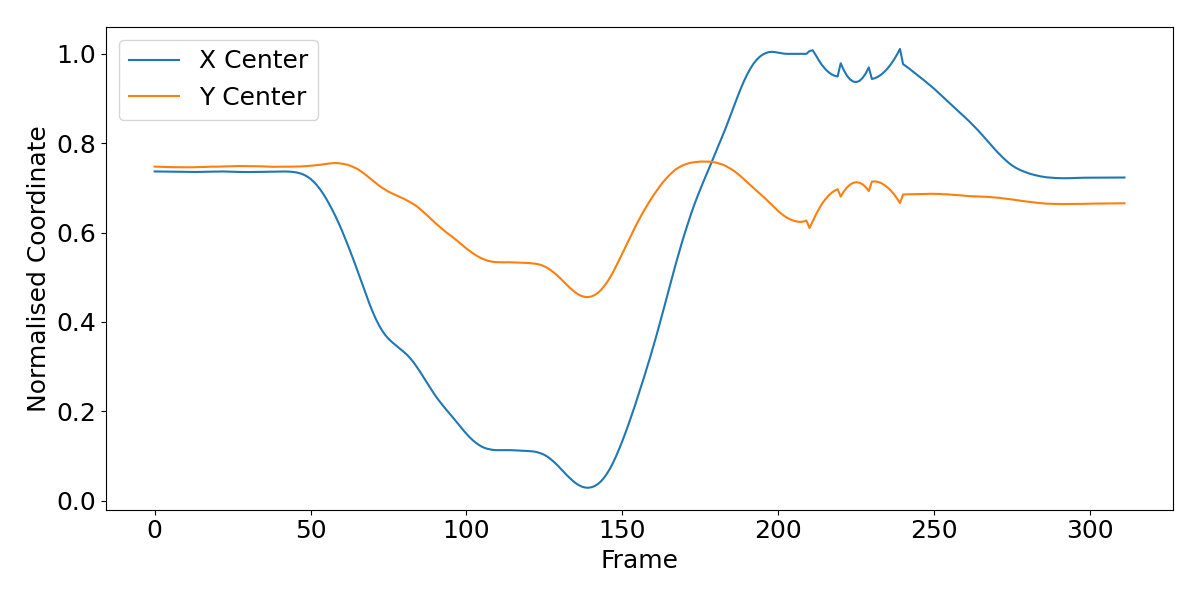
\includegraphics[width=\textwidth]{figures/bbox_metrics/test_indoor1 (Savgol Filter)_central_position.png}
        \caption{Central position of the refueling port over time.}
        \label{fig:central-position-test-indoor1-savgol}
    \end{subfigure}
    \hfill
    \begin{subfigure}[t]{0.6\textwidth}
        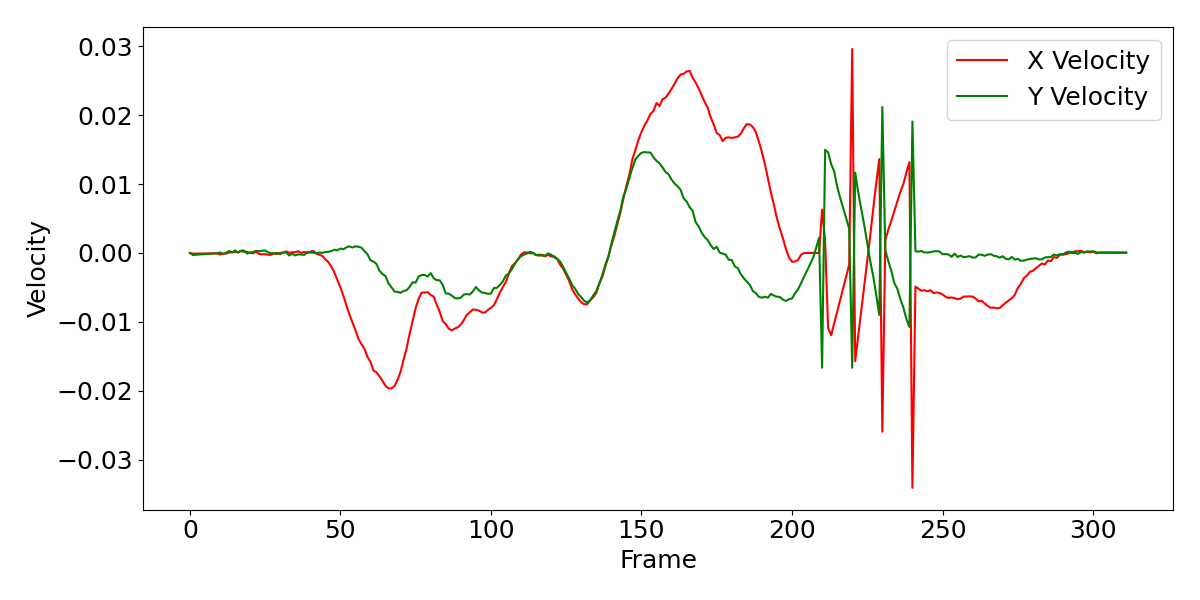
\includegraphics[width=\textwidth]{figures/bbox_metrics/test_indoor1 (Savgol Filter)_velocity.png}
        \caption{Velocity of the refueling port over time.}
        \label{fig:velocity-test-indoor1-savgol}
    \end{subfigure}
    \vfill
    \begin{subfigure}[t]{0.6\textwidth}
        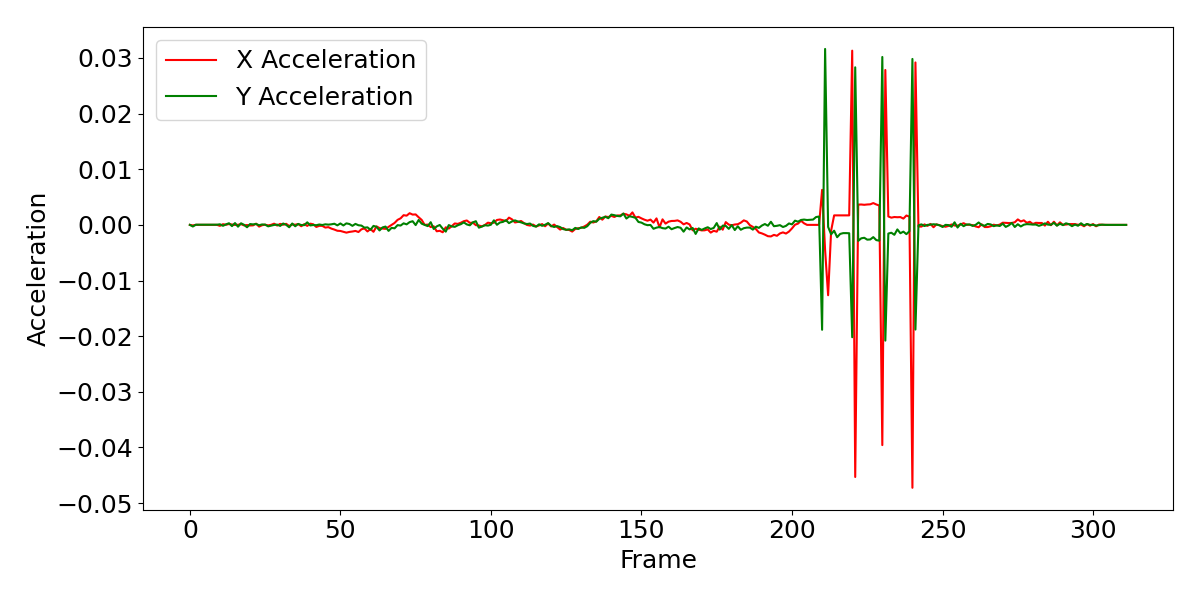
\includegraphics[width=\textwidth]{figures/bbox_metrics/test_indoor1 (Savgol Filter)_acceleration.png}
        \caption{Acceleration of the refueling port over time.}
        \label{fig:acceleration-test-indoor1-savgol}
    \end{subfigure}
    \hfill
    \begin{subfigure}[t]{0.6\textwidth}
        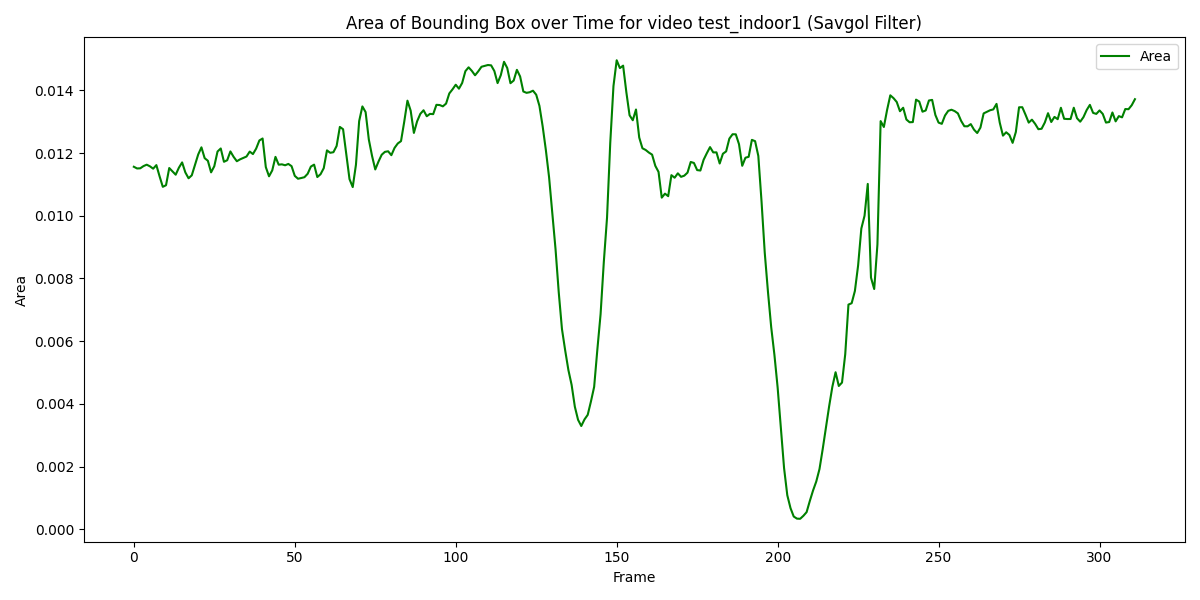
\includegraphics[width=\textwidth]{figures/bbox_metrics/test_indoor1 (Savgol Filter)_area.png}
        \caption{Area of the refueling port over time.}
        \label{fig:size-test-indoor1-savgol}
    \end{subfigure}
    \caption{Temporal analysis of different metrics for the refueling port in the \textit{test\_indoor1} video. The metrics include (a) central position, (b) velocity, (c) acceleration, and (d) area, providing a comprehensive overview of the object's dynamics over time.}
    \label{fig:bbox-metrics-test-indoor1-savgol}
\end{figure}

\begin{figure}[H]
    \centering
    \begin{subfigure}[t]{0.6\textwidth}
        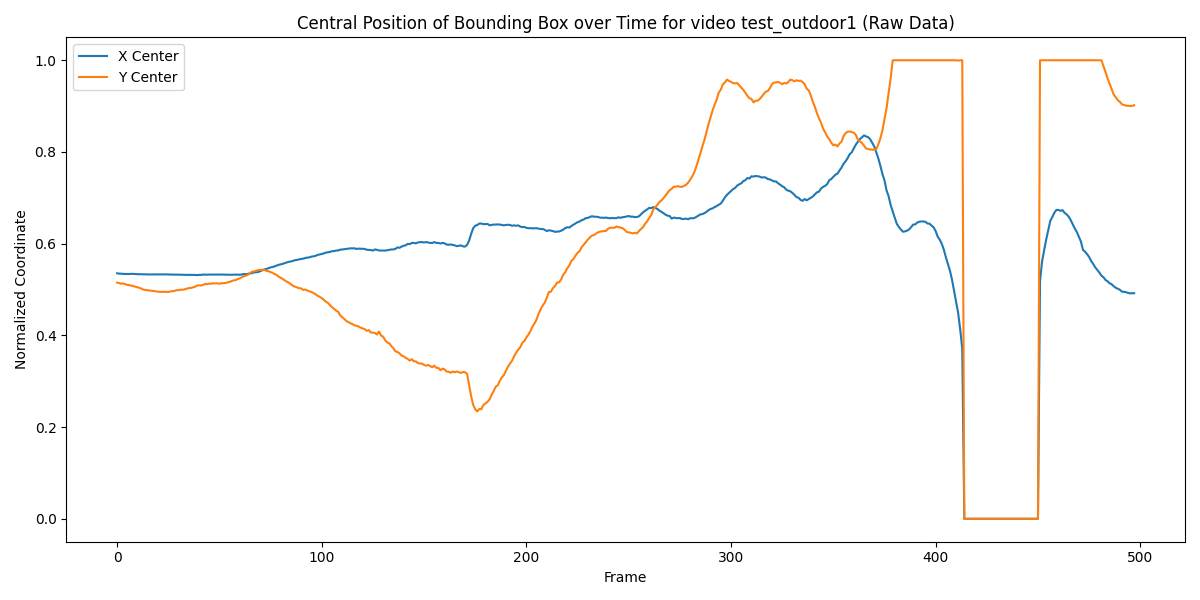
\includegraphics[width=\textwidth]{figures/bbox_metrics/test_outdoor1 (Raw Data)_central_position.png}
        \caption{Central position of the refueling port over time.}
        \label{fig:central-position-test-outdoor1}
    \end{subfigure}
    \hfill
    \begin{subfigure}[t]{0.6\textwidth}
        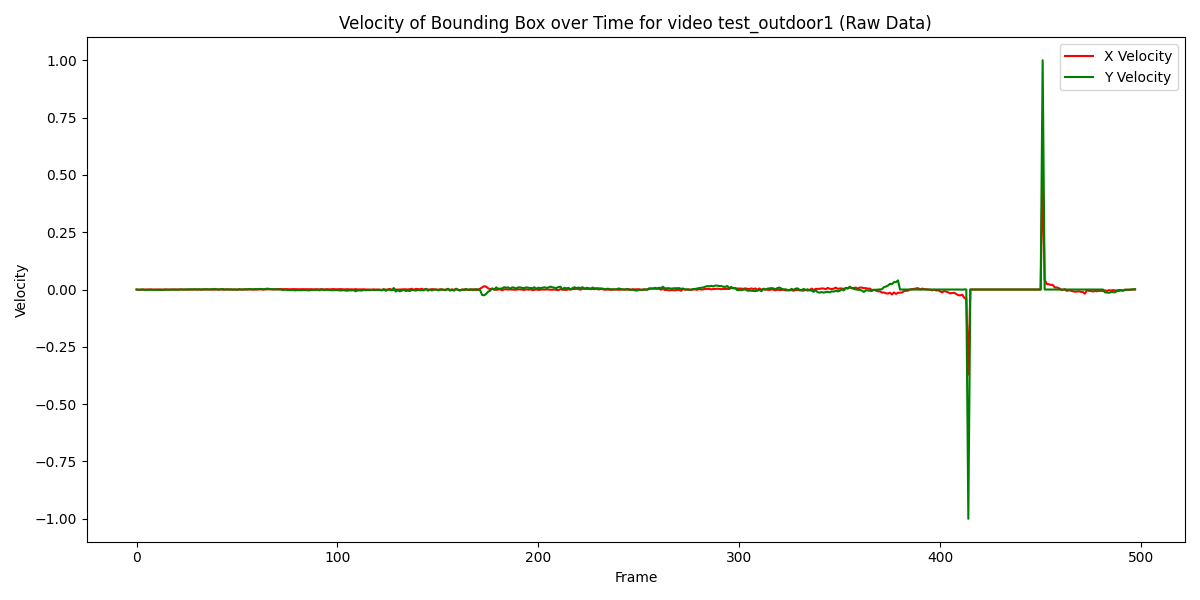
\includegraphics[width=\textwidth]{figures/bbox_metrics/test_outdoor1 (Raw Data)_velocity.png}
        \caption{Velocity of the refueling port over time.}
        \label{fig:velocity-test-outdoor1}
    \end{subfigure}
    \vfill
    \begin{subfigure}[t]{0.6\textwidth}
        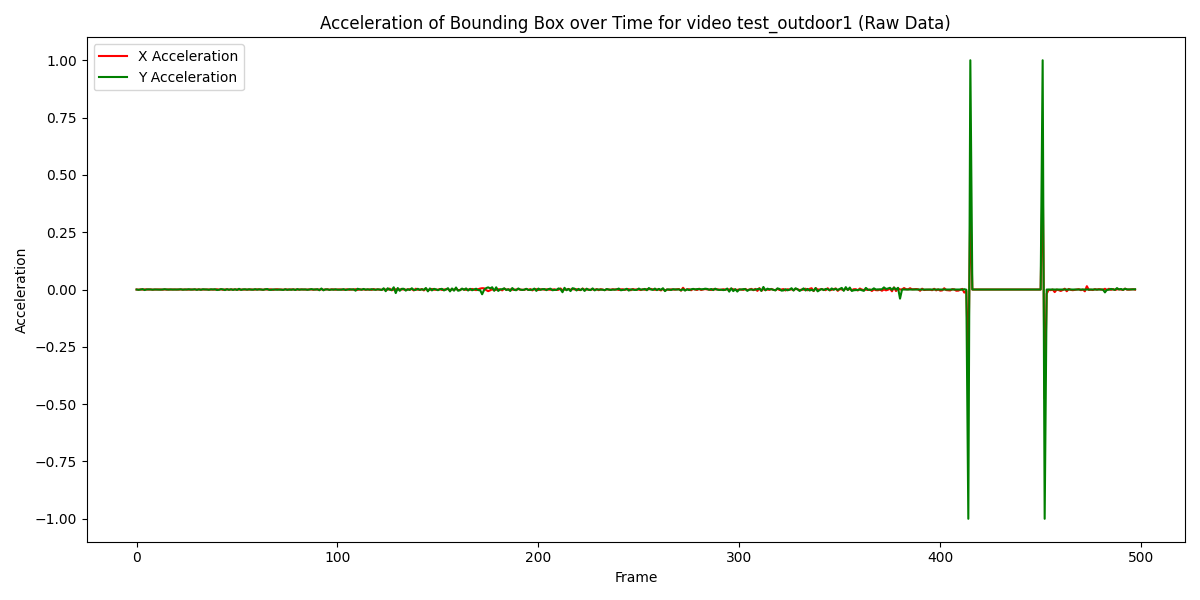
\includegraphics[width=\textwidth]{figures/bbox_metrics/test_outdoor1 (Raw Data)_acceleration.png}
        \caption{Acceleration of the refueling port over time.}
        \label{fig:acceleration-test-outdoor1}
    \end{subfigure}
    \hfill
    \begin{subfigure}[t]{0.6\textwidth}
        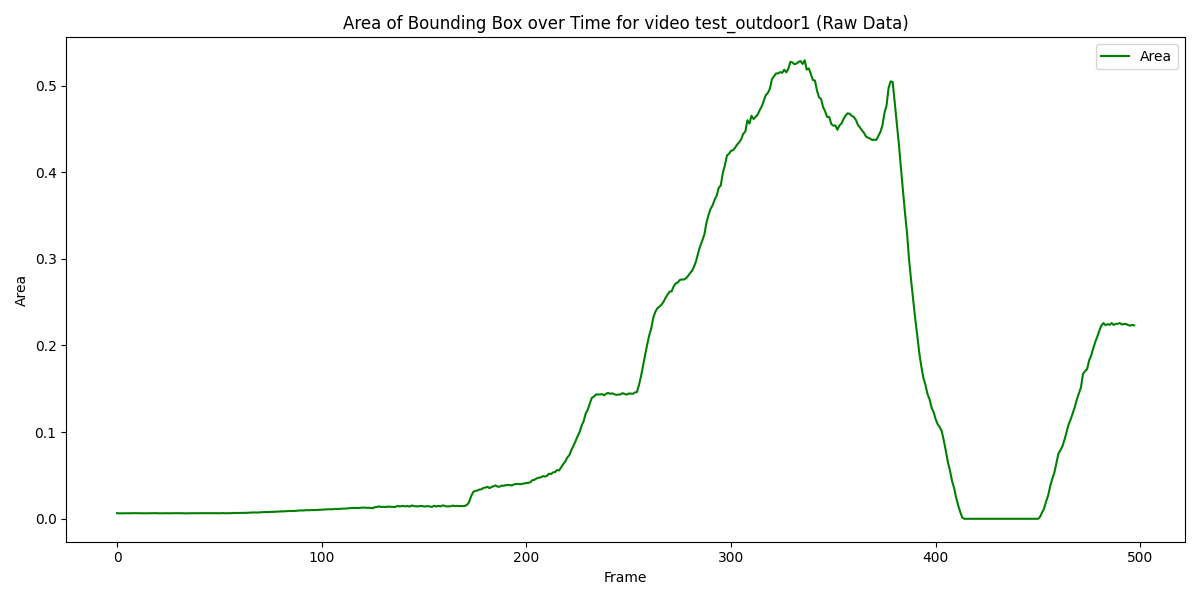
\includegraphics[width=\textwidth]{figures/bbox_metrics/test_outdoor1 (Raw Data)_area.png}
        \caption{Area of the refueling port over time.}
        \label{fig:size-test-outdoor1}
    \end{subfigure}
    \caption{Temporal analysis of different metrics for the refueling port in the \textit{test\_outdoor1} video. The metrics include (a) central position, (b) velocity, (c) acceleration, and (d) area, providing a comprehensive overview of the object's dynamics over time.}
    \label{fig:bbox-metrics-test-outdoor1}
\end{figure}

\begin{figure}[H]
    \centering
    \begin{subfigure}[t]{0.6\textwidth}
        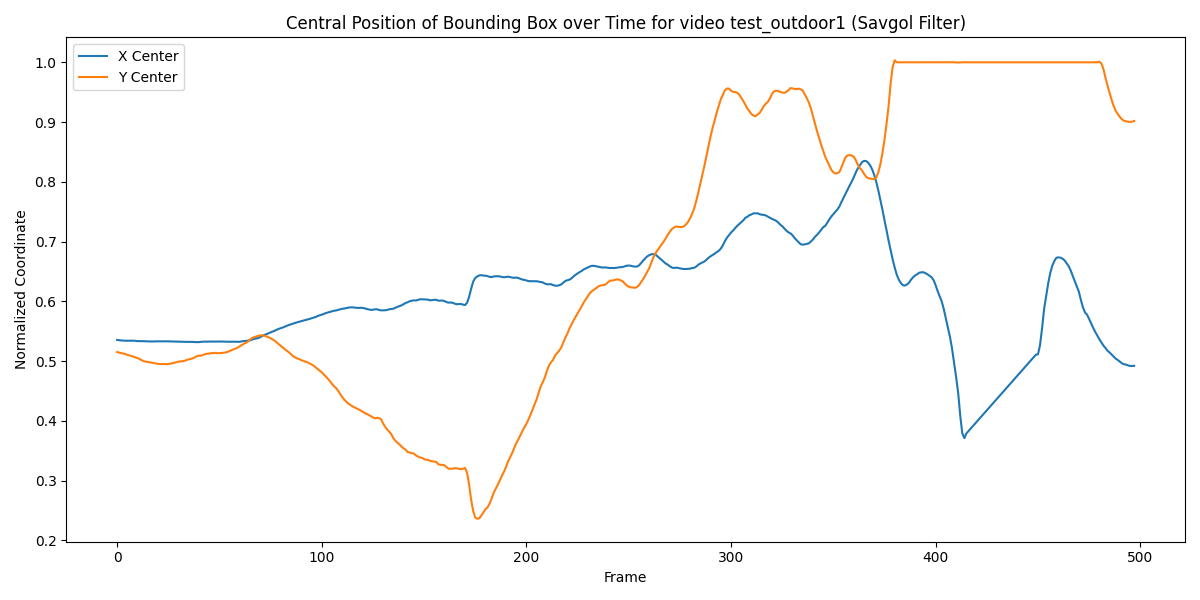
\includegraphics[width=\textwidth]{figures/bbox_metrics/test_outdoor1 (Savgol Filter)_central_position.png}
        \caption{Central position of the refueling port over time.}
        \label{fig:central-position-test-outdoor1-savgol}
    \end{subfigure}
    \hfill
    \begin{subfigure}[t]{0.6\textwidth}
        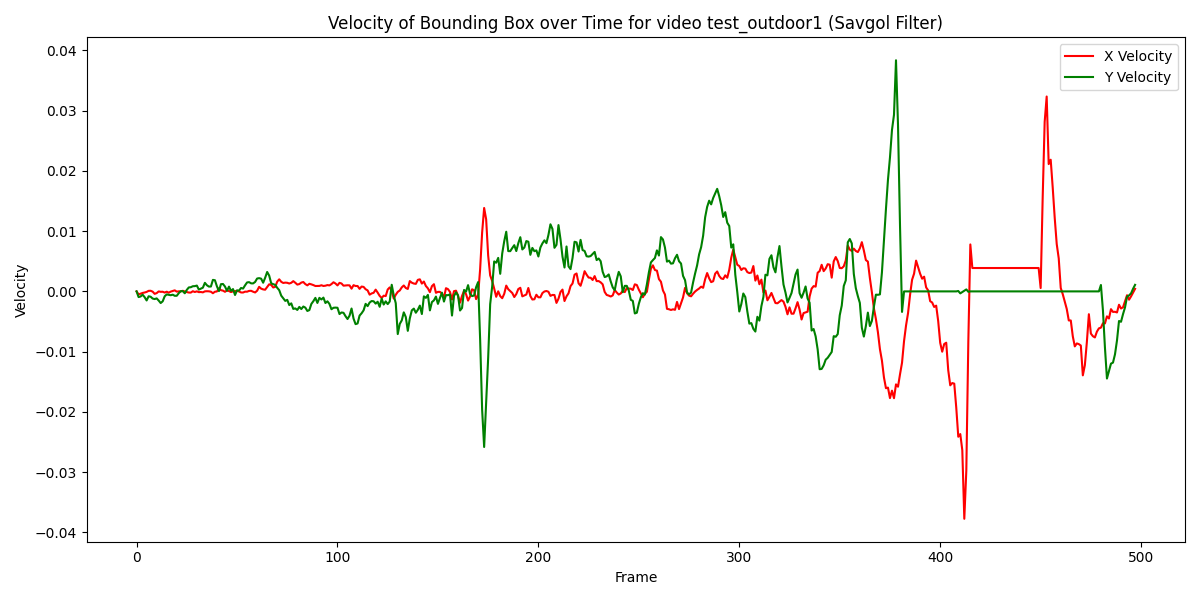
\includegraphics[width=\textwidth]{figures/bbox_metrics/test_outdoor1 (Savgol Filter)_velocity.png}
        \caption{Velocity of the refueling port over time.}
        \label{fig:velocity-test-outdoor1-savgol}
    \end{subfigure}
    \vfill
    \begin{subfigure}[t]{0.6\textwidth}
        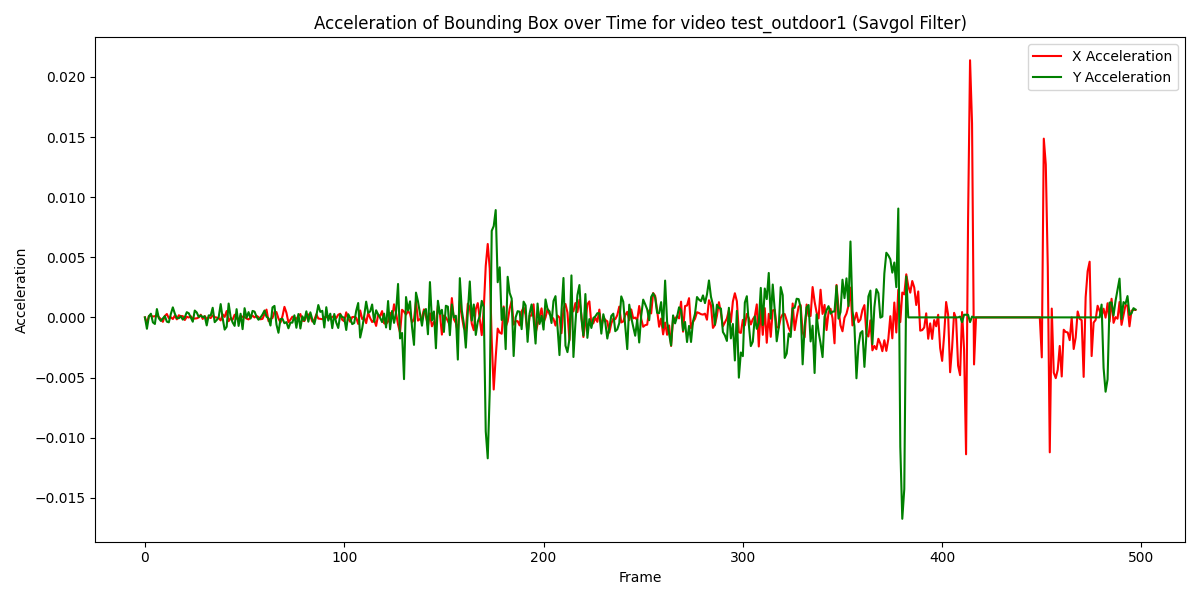
\includegraphics[width=\textwidth]{figures/bbox_metrics/test_outdoor1 (Savgol Filter)_acceleration.png}
        \caption{Acceleration of the refueling port over time.}
        \label{fig:acceleration-test-outdoor1-savgol}
    \end{subfigure}
    \hfill
    \begin{subfigure}[t]{0.6\textwidth}
        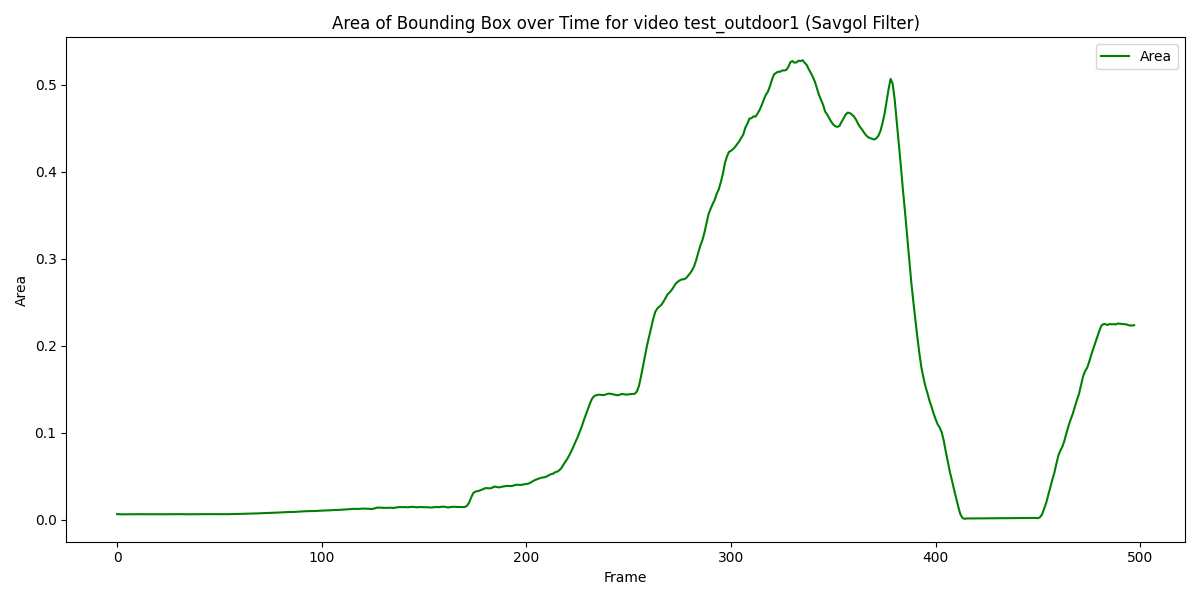
\includegraphics[width=\textwidth]{figures/bbox_metrics/test_outdoor1 (Savgol Filter)_area.png}
        \caption{Area of the refueling port over time.}
        \label{fig:size-test-outdoor1-savgol}
    \end{subfigure}
    \caption{Temporal analysis of different metrics for the refueling port in the \textit{test\_outdoor1} video. The metrics include (a) central position, (b) velocity, (c) acceleration, and (d) area, providing a comprehensive overview of the object's dynamics over time.}
    \label{fig:bbox-metrics-test-outdoor1-savgol}
\end{figure}

\begin{figure}[H]
    \centering
    \begin{subfigure}[t]{0.6\textwidth}
        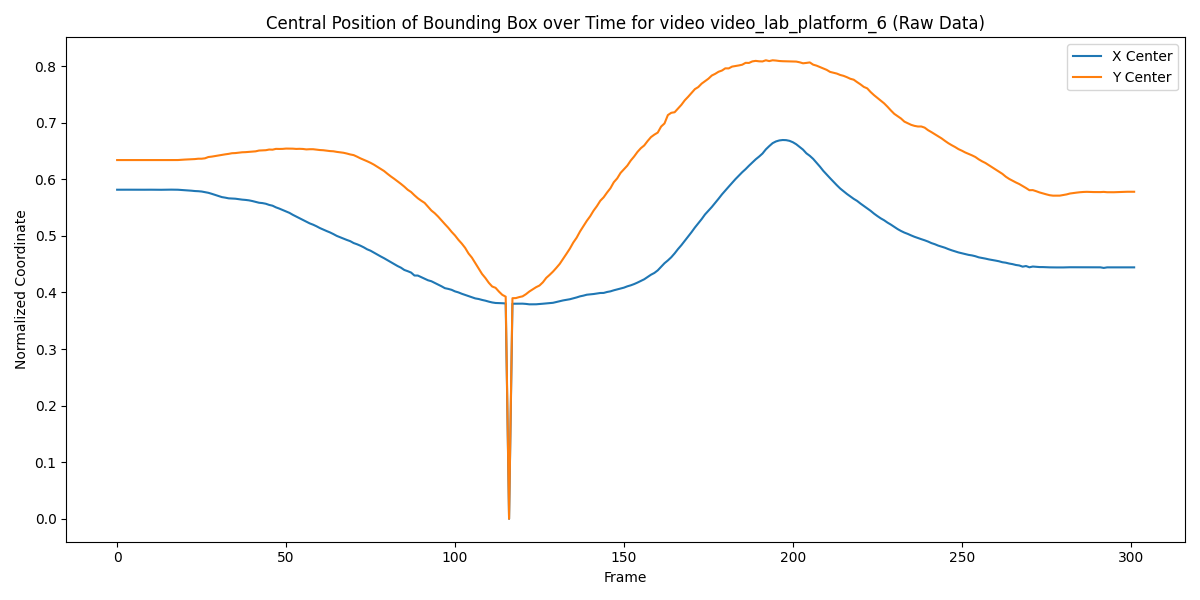
\includegraphics[width=\textwidth]{figures/bbox_metrics/video_lab_platform_6 (Raw Data)_central_position.png}
        \caption{Central position of the refueling port over time.}
        \label{fig:central-position-test-video_lab_platform_6}
    \end{subfigure}
    \hfill
    \begin{subfigure}[t]{0.6\textwidth}
        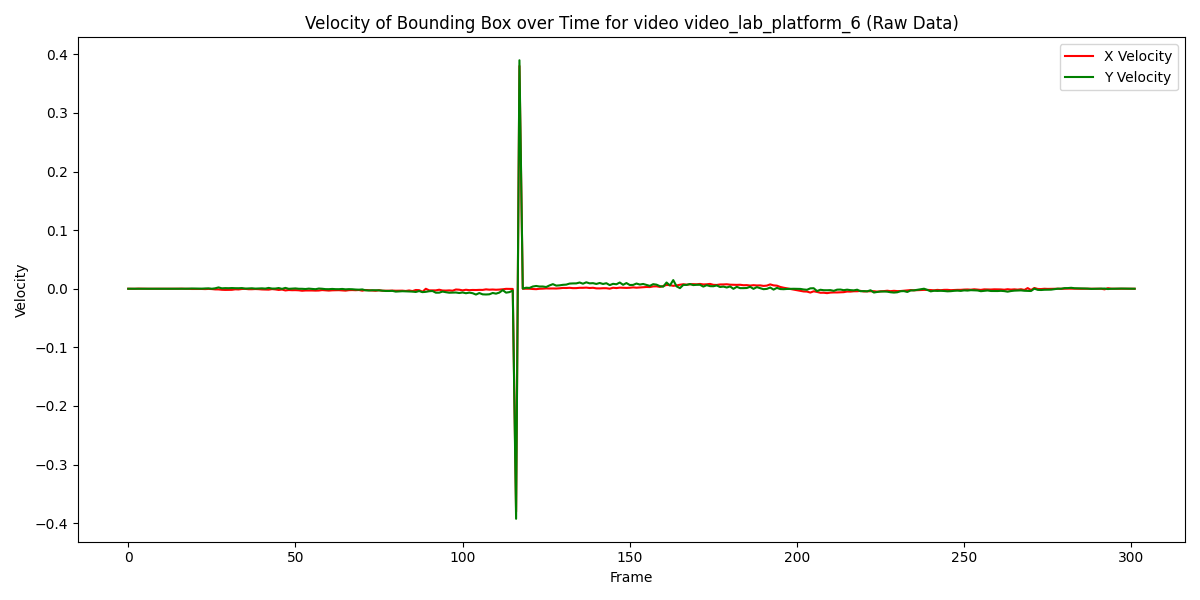
\includegraphics[width=\textwidth]{figures/bbox_metrics/video_lab_platform_6 (Raw Data)_velocity.png}
        \caption{Velocity of the refueling port over time.}
        \label{fig:velocity-test-video_lab_platform_6}
    \end{subfigure}
    \vfill
    \begin{subfigure}[t]{0.6\textwidth}
        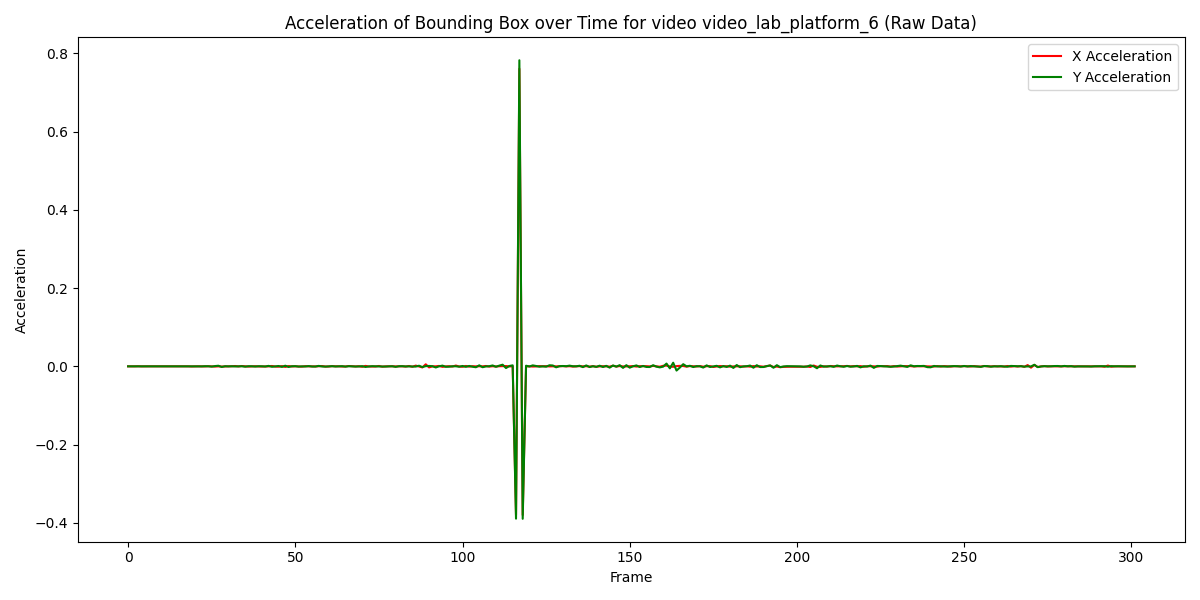
\includegraphics[width=\textwidth]{figures/bbox_metrics/video_lab_platform_6 (Raw Data)_acceleration.png}
        \caption{Acceleration of the refueling port over time.}
        \label{fig:acceleration-test-video_lab_platform_6}
    \end{subfigure}
    \hfill
    \begin{subfigure}[t]{0.6\textwidth}
        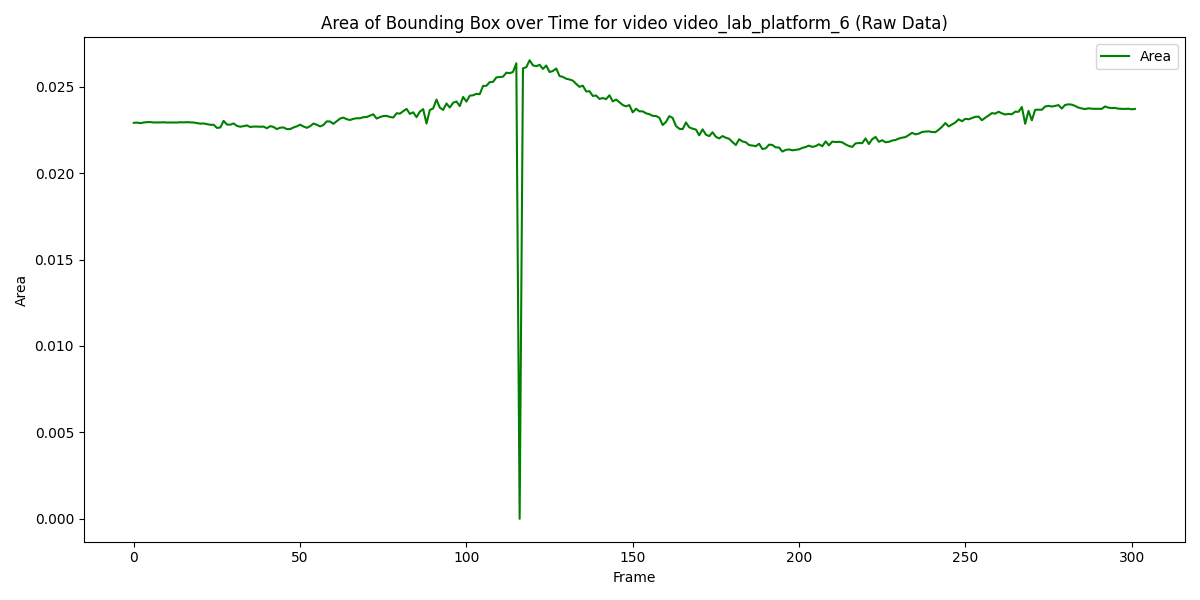
\includegraphics[width=\textwidth]{figures/bbox_metrics/video_lab_platform_6 (Raw Data)_area.png}
        \caption{Area of the refueling port over time.}
        \label{fig:size-test-video_lab_platform_6}
    \end{subfigure}
    \caption{Temporal analysis of different metrics for the refueling port in the \textit{test\_video\_lab\_platform\_6} video. The metrics include (a) central position, (b) velocity, (c) acceleration, and (d) area, providing a comprehensive overview of the object's dynamics over time.}
    \label{fig:bbox-metrics-test-video_lab_platform_6}
\end{figure}

\begin{figure}[H]
    \centering
    \begin{subfigure}[t]{0.6\textwidth}
        \includegraphics[width=\textwidth]{figures/bbox_metrics/video_lab_platform_6 (Savgol Filter)_central_position.png}
        \caption{Central position of the refueling port over time.}
        \label{fig:central-position-test-video_lab_platform_6-savgol}
    \end{subfigure}
    \hfill
    \begin{subfigure}[t]{0.6\textwidth}
        \includegraphics[width=\textwidth]{figures/bbox_metrics/video_lab_platform_6 (Savgol Filter)_velocity.png}
        \caption{Velocity of the refueling port over time.}
        \label{fig:velocity-test-video_lab_platform_6-savgol}
    \end{subfigure}
    \vfill
    \begin{subfigure}[t]{0.6\textwidth}
        \includegraphics[width=\textwidth]{figures/bbox_metrics/video_lab_platform_6 (Savgol Filter)_acceleration.png}
        \caption{Acceleration of the refueling port over time.}
        \label{fig:acceleration-test-video_lab_platform_6-savgol}
    \end{subfigure}
    \hfill
    \begin{subfigure}[t]{0.6\textwidth}
        \includegraphics[width=\textwidth]{figures/bbox_metrics/video_lab_platform_6 (Savgol Filter)_area.png}
        \caption{Area of the refueling port over time.}
        \label{fig:size-test-video_lab_platform_6-savgol}
    \end{subfigure}
    \caption{Temporal analysis of different metrics for the refueling port in the \textit{test\_video\_lab\_platform\_6} video. The metrics include (a) central position, (b) velocity, (c) acceleration, and (d) area, providing a comprehensive overview of the object's dynamics over time.}
    \label{fig:bbox-metrics-test-video_lab_platform_6-savgol}
\end{figure}

\subsection{Framework Design Overview}
The proposed framework (see figure~\ref{fig:framework-workflow}) aims to
predict the future bounding boxes of the refueling port over the next \(m\)
frames of a video stream, using the observed bounding boxes from the current
and previous frames. The observed bounding box at time step \(t\) is
represented as \(\mathbf{b}_t = [x_t, y_t, w_t, h_t]\), where \((x_t, y_t)\)
denotes the coordinates of the bounding box center, and \(w_t\) and \(h_t\)
represent the width and height of the bounding box, respectively. The objective
is to predict a sequence of future bounding boxes \(\mathbf{S}_{t+1:t+m} =
\{\mathbf{b}_{t+1}, \dots, \mathbf{b}_{t+m}\}\) on the following \(m\) frames,
based on the past \(n\) observed bounding boxes \(\mathbf{S}_{t-1+n:t} =
\{\mathbf{b}_{t-1+n}, \dots, \mathbf{b}_{t}\}\). 

The frame process begins with the input video sequence, which is analysed frame
by frame. An object detection model identifies and locates the bounding boxes
of the supply port. These bounding boxes are then used in subsequent stages of
data processing.

Two key input vectors are extracted from the bounding box information: the
\textit{spatial dynamics vector} and the \textit{dimensional attributes
    vector}. The spatial dynamics vector includes information about the position,
velocity, and acceleration of the bounding box center, represented as
\(\mathbf{p}_t = [x_t, y_t, v_{x,t}, v_{y,t}, a_{x,t}, a_{y,t}]\). The
dimensional attributes vector captures the size of the bounding box and the
changes in its dimensions over time, expressed as \(\mathbf{d}_t = [w_t, h_t,
\Delta w_t, \Delta h_t]\).

These input vectors are fed into a sequence model, where they are processed
through separate encoders to extract meaningful temporal features. The encoded
features are then concatenated and passed to a decoder, which predicts the
future bounding boxes for the refueling port across the next \(N\) frames. The
resulting output, \(\mathbf{B}_{t} = \{\mathbf{b}_{t+1}, \dots,
\mathbf{b}_{t+N}\}\), provides an estimate of the bounding box positions and
sizes in the subsequent frames.

This method effectively leverages both the spatial and dimensional information
of the bounding boxes to generate accurate predictions of future positions and
sizes, which are essential for tasks such as object tracking and navigation.

\begin{figure}[H]
    \centering
    \includegraphics[width=0.7\textwidth]{figures/FrameworkWorkflow.drawio.pdf}
    \caption{Framework Workflow}\label{fig:framework-workflow}
\end{figure}

The proposed framework consists of two main components: an object detection
model and a sequence model. The object detection model is responsible for
detecting the refueling port in each frame of the video, while the sequence
model predicts the future positions and sizes of the detected refueling port.
The framework workflow is illustrated in Figure~\ref{fig:framework-workflow}. 

\subsection{Object Detection Model}
The object detection model provides a sequence of bounding boxes in each video
frame, represented in the following format:
\[
    (x_{\text{center}}, y_{\text{center}}, w, h),
\]
where $(x_{\text{center}}, y_{\text{center}})$ denotes the coordinates of the
bounding box center, and $(w, h)$ represent the width and height of the
bounding box, respectively.

\section{Sequence Model Design}

\begin{figure}[H]
    \centering
    \includegraphics[width=1\textwidth]{figures/GRUSizPos.drawio.pdf}
    \caption{SizPos-GRU Model Architecture}\label{fig:sizpos-gru}
\end{figure}

This thesis introduces the SizPos-GRU model, a deep learning sequence model for
predicting future positions and sizes of a unique object in a video stream. The
model leverages an encoder-attention-decoder architecture to capture temporal
dependencies and spatial relationships effectively. The framework consists of
four main components: two encoders, an attention mechanism, and two decoders.
Each component is designed to handle specific aspects of the sequence modeling
task, from encoding input sequences to generating context-aware predictions.

\subsection{Input Representation}
The \textit{SizPos-GRU} model expects two types of input sequences to predict
the future positions and sizes of an object. The first input captures the
spatial dynamics of the object, including its position, velocity and
acceleration. The second input focuses on the object's dimensional attributes,
such as its width and height, and changes in these dimensions over time.

\subsubsection{Spatial Dynamics Vector}
The spatial dynamics vector at time $t$, denoted as $\mathbf{p}_t$, is obtained
by computing the position, velocity, and acceleration of the bounding box
center:
\begin{align}
    \mathbf{p}_t & = \left(x_t, y_t, v_{x,t}, v_{y,t}, a_{x,t}, a_{y,t}\right), \\
    v_{x,t}      & = x_t - x_{t-1}, \quad v_{y,t} = y_t - y_{t-1},              \\
    a_{x,t}      & = v_{x,t} - v_{x,t-1}, \quad a_{y,t} = v_{y,t} - v_{y,t-1}.
\end{align}
Here, $(x_t, y_t)$ represents the center coordinates at time $t$, $(v_{x,t}, v_{y,t})$ are the velocities, and $(a_{x,t}, a_{y,t})$ are the accelerations along the $x$ and $y$ axes.

\subsubsection{Dimensional Attributes Vector}
The dimensional attributes vector at time $t$, denoted as $\mathbf{d}_t$,
captures the size of the bounding box and the changes in its dimensions:
\begin{align}
    \mathbf{d}_t & = \left(w_t, h_t, \Delta w_t, \Delta h_t\right),    \\
    \Delta w_t   & = w_t - w_{t-1}, \quad \Delta h_t = h_t - h_{t-1}.
\end{align}
Here, $(w_t, h_t)$ represents the width and height at time $t$, and $(\Delta w_t, \Delta h_t)$ are the changes in these dimensions from the previous time step.

\subsubsection{Input Sequences for Model}
The sequences of these vectors over a time window $T$ are fed into the model
as:
\[
    \mathbf{P} = \{\mathbf{p}_1, \mathbf{p}_2, \dots, \mathbf{p}_T\}, \quad \mathbf{D} = \{\mathbf{d}_1, \mathbf{d}_2, \dots, \mathbf{d}_T\},
\]
where $\mathbf{P}$ is the sequence of spatial dynamics vectors and $\mathbf{D}$
is the sequence of dimensional attributes vectors. These sequences are then
processed by the model's encoders to extract temporal features for predicting
future bounding box positions and sizes.

These sequences are fed into the encoders to extract meaningful temporal
features.

\subsubsection{Encoders}
The framework employs two separate LSTM encoders: one for processing the
sequence of bounding boxes and another for processing the sequence of
velocities. Each encoder is designed to capture the temporal dependencies
within its respective input data.

The bounding box encoder is defined as:

\begin{equation}
    H_p, (h_{p_n}, c_{p_n}) = \text{LSTM}_p(\mathbf{P})
\end{equation}

where $\mathbf{P} = (\mathbf{p}_1, \mathbf{p}_2, \ldots, \mathbf{p}_T)$ is the
input sequence of bounding boxes, $H_p = (h_{p_1}, h_{p_2}, \ldots, h_{p_T})$
represents the sequence of hidden states, and $(h_{p_n}, c_{p_n})$ are the
final hidden and cell states of the bounding box encoder.

The velocity encoder is defined as:

\begin{equation}
    H_v, (h_{v_n}, c_{v_n}) = \text{LSTM}_v(\mathbf{V})
\end{equation}

where $\mathbf{V} = (\mathbf{v}_1, \mathbf{v}_2, \ldots, \mathbf{v}_T)$ is the
input sequence of velocities, $H_v = (h_{v_1}, h_{v_2}, \ldots, h_{v_T})$
represents the sequence of hidden states, and $(h_{v_n}, c_{v_n})$ are the
final hidden and cell states of the velocity encoder.

\subsubsection{Attention Mechanism}

The attention mechanism is crucial for allowing the model to focus on relevant
parts of the input sequences when making predictions. It computes a set of
attention weights that highlight important hidden states from both encoders.
These weights are used to form context vectors, which provide the decoders with
relevant information from the input sequences.

The attention weights $\alpha_t$ are calculated as follows:

\begin{equation}
    \alpha_t = \text{softmax}(v^\top \tanh(W_{h_p} H_p + W_{h_v} H_v + W_s s_{t-1}))
\end{equation}

where $W_{h_p}$ and $W_{h_v}$ are learned weight matrices for the bounding box
and velocity hidden states, respectively, $W_s$ is a learned weight matrix for
the previous decoder state, and $v$ is a learned vector. The context vectors
$c_{p_t}$ and $c_{v_t}$ are then computed as:

\begin{equation}
    c_{p_t} = \sum_{i=1}^{T} \alpha_{t,i} h_{p_i}
\end{equation}

\begin{equation}
    c_{v_t} = \sum_{i=1}^{T} \alpha_{t,i} h_{v_i}
\end{equation}

These context vectors are passed to the decoders to generate the next time step
predictions.

\subsection{Decoders}
The framework employs two separate LSTM decoders: one for generating
predictions for future bounding boxes and another for generating predictions
for future velocities. Each decoder takes as input the previous output and the
context vectors from the attention mechanism.

The bounding box decoder's input at each time step $t$ is the concatenated
vector of the previous output and the context vector from the bounding box
encoder:

\begin{equation}
    \mathbf{d}_{p_t} = [\mathbf{p}_{t-1}, c_{p_{t-1}}]
\end{equation}

The LSTM in the bounding box decoder processes this input to update its hidden
and cell states:

\begin{equation}
    s_{p_t}, (h_{p_t}, c_{p_t}) = \text{LSTM}_p(\mathbf{d}_{p_t}, (h_{p_{t-1}}, c_{p_{t-1}}))
\end{equation}

The final output for the bounding box is obtained through a fully connected
layer with a sigmoid activation function to ensure the output values are
between 0 and 1:

\begin{equation}
    \mathbf{p}_t = \text{Sigmoid}(\text{Linear}_p(s_{p_t}))
\end{equation}

Similarly, the velocity decoder's input at each time step $t$ is the
concatenated vector of the previous output and the context vector from the
velocity encoder:

\begin{equation}
    \mathbf{d}_{v_t} = [\mathbf{v}_{t-1}, c_{v_{t-1}}]
\end{equation}

The LSTM in the velocity decoder processes this input to update its hidden and
cell states:

\begin{equation}
    s_{v_t}, (h_{v_t}, c_{v_t}) = \text{LSTM}_v(\mathbf{d}_{v_t}, (h_{v_{t-1}}, c_{v_{t-1}}))
\end{equation}

The final output for the velocity is obtained through a fully connected layer
without any activation function. This design choice allows the output values to
range freely, including negative values, which is necessary because velocities
can be positive or negative:

\begin{equation}
    \mathbf{v}_t = \text{Linear}_v(s_{v_t})
\end{equation}

The decoders continue this process for the entire prediction horizon, using
their own previous outputs as inputs for future predictions.

\subsection{Transformer-Based Architecture}

The proposed model leverages a Transformer architecture to predict future
positions and velocities of objects in a video stream. Transformers, introduced
by Vaswani et al. (2017), have demonstrated superior performance in
sequence-to-sequence tasks by effectively capturing long-range dependencies
through self-attention mechanisms. Our architecture consists of three main
components: an encoder, a decoder, and a multi-head self-attention mechanism.
Each component is designed to handle specific aspects of the sequence modeling
task, from encoding input sequences to generating context-aware predictions.

\subsubsection{Input Representation}

The model takes as input sequences of bounding boxes and their velocities
extracted from video frames. Each bounding box is represented by its center
coordinates $(x_{\text{center}}, y_{\text{center}})$, width $(w)$, and height
$(h)$. Corresponding velocities are represented by changes in these values:
$(\Delta x, \Delta y, \Delta w, \Delta h)$. Thus, each input vector
$\mathbf{p}_t$ and $\mathbf{v}_t$ at time $t$ can be represented as:

\begin{equation}
    \mathbf{p}_t = (x_{\text{center}, t}, y_{\text{center}, t}, w_t, h_t)
\end{equation}

\begin{equation}
    \mathbf{v}_t = (\Delta x_t, \Delta y_t, \Delta w_t, \Delta h_t)
\end{equation}

These sequences are fed into the encoder to extract meaningful temporal
features.

\subsubsection{Encoder}

The encoder consists of multiple layers, each containing two main components: a
multi-head self-attention mechanism and a position-wise fully connected
feed-forward network. The input to the encoder is a sequence of bounding box
and velocity vectors. The encoder processes these sequences independently using
the following steps:

\begin{itemize}
    \item \textbf{Positional Encoding}: Since the Transformer model does not have a built-in notion of order, positional encodings are added to the input embeddings to incorporate sequence order information.
    \item \textbf{Self-Attention}: The multi-head self-attention mechanism allows the model to focus on different parts of the input sequence simultaneously, capturing dependencies regardless of their distance in the sequence.
    \item \textbf{Feed-Forward Network}: A position-wise fully connected feed-forward network is applied to the output of the self-attention mechanism to introduce non-linearity and further process the information.
    \item \textbf{Residual Connection and Layer Normalization}: Residual connections around each sub-layer followed by layer normalization help in stabilizing the training and improving gradient flow.
\end{itemize}

\subsubsection{Decoder}

The decoder is similarly composed of multiple layers, with each layer
containing three main components: a multi-head self-attention mechanism, a
multi-head encoder-decoder attention mechanism, and a position-wise fully
connected feed-forward network. The decoder generates predictions for future
bounding boxes and velocities using the following steps:

\begin{itemize}
    \item \textbf{Masked Self-Attention}: The decoder's self-attention mechanism is masked to prevent positions from attending to subsequent positions, ensuring that the prediction for a position depends only on known outputs.
    \item \textbf{Encoder-Decoder Attention}: This mechanism allows the decoder to focus on relevant parts of the encoder's output, providing context from the input sequence.
    \item \textbf{Feed-Forward Network}: Similar to the encoder, a fully connected feed-forward network is applied to the output of the attention mechanisms.
    \item \textbf{Residual Connection and Layer Normalization}: As in the encoder, residual connections and layer normalization are applied to stabilize training and improve gradient flow.
\end{itemize}

\subsubsection{Multi-Head Self-Attention}

The multi-head self-attention mechanism is a key component of the Transformer
architecture, enabling the model to jointly attend to information from
different representation subspaces. It works by projecting the input sequence
into multiple sets of queries, keys, and values, performing scaled dot-product
attention for each set, and concatenating the results. This process allows the
model to capture various aspects of the input sequence, enhancing its ability
to learn complex patterns.

\subsubsection{Output Generation}

The output of the decoder is passed through a linear layer to generate
predictions for the bounding box coordinates and velocities. Separate linear
layers are used for bounding box predictions (with a sigmoid activation to
ensure values are between 0 and 1) and velocity predictions (without activation
to allow for positive and negative values).

\subsubsection{Loss Function and Training}

The model is trained to minimize the mean squared error between the predicted
and actual bounding boxes and velocities. The loss function is defined as:

\begin{equation}
    \text{Loss} = \frac{1}{N} \sum_{i=1}^{N} \sum_{t=1}^{T} \left[ (x_{i,t} - \hat{x}_{i,t})^2 + (y_{i,t} - \hat{y}_{i,t})^2 + (w_{i,t} - \hat{w}_{i,t})^2 + (h_{i,t} - \hat{h}_{i,t})^2 + (\Delta x_{i,t} - \hat{\Delta x}_{i,t})^2 + (\Delta y_{i,t} - \hat{\Delta y}_{i,t})^2 + (\Delta w_{i,t} - \hat{\Delta w}_{i,t})^2 + (\Delta h_{i,t} - \hat{\Delta h}_{i,t})^2 \right]
\end{equation}

The Adam optimizer is used to update the model parameters, and early stopping
based on validation loss is employed to prevent overfitting and ensure
generalization.

\section{Algorithm Design}

\section{Data Augmentation Strategy}

The data augmentation strategy is designed to enhance the robustness and
generalization capability of the model. This strategy simulates various camera
movements and imperfections that might occur in real-world scenarios. The
augmentation approach consists of the following key components:

\subsection{Sequence Reversal}

For the training stage, the size of the dataset is doubled by including
reversed sequences:

\begin{itemize}
    \item For each original sequence $(S_1, S_2, ..., S_n)$, a reversed sequence $(S_n,
              S_{n-1}, ..., S_1)$ is added.
    \item This augmentation helps the model learn to predict both forward and backward
          movements of the camera relative to the aircraft refueling port.
\end{itemize}

\subsection{Camera Movement Simulation}

Subtle camera movements are simulated to make the model more robust to varying
camera positions:

\begin{itemize}
    \item \textbf{Panning}: A smooth, cumulative random offset is applied to the x and y coordinates of the bounding boxes. This simulates the effect of the camera panning horizontally or vertically.
    \item The panning effect is modeled as:
          \begin{equation}
              \text{pan}_t = \sum_{i=1}^t \frac{N(0, \sigma^2)}{5}
          \end{equation}
          where $N(0, \sigma^2)$ is a normal distribution with mean 0 and variance $\sigma^2$.
\end{itemize}

\subsection{Zoom Simulation}

To account for changes in the apparent size of the refueling port due to camera
zoom or aircraft movement:

\begin{itemize}
    \item A smooth, cumulative scaling factor is applied to the width and height of the
          bounding boxes.
    \item The zoom effect is modeled as:
          \begin{equation}
              \text{zoom}_t = \prod_{i=1}^t U(0.98, 1.02)
          \end{equation}
          where $U(0.98, 1.02)$ is a uniform distribution between 0.98 and 1.02.
\end{itemize}

\subsection{Detection Inaccuracy Simulation}

To make the model more robust to slight inaccuracies in object detection:

\begin{itemize}
    \item Small Gaussian noise is added to all bounding box coordinates.
    \item The noise is sampled from $N(0, 0.002^2)$ for each coordinate.
\end{itemize}

\subsection{Implementation Details}

The augmentation strategy is applied with the following considerations:

\begin{itemize}
    \item Augmentations are only applied during the training stage.
    \item Each sequence has a 50\% chance of being augmented.
    \item When applied, augmentations affect both input and output sequences consistently
          to maintain temporal coherence.
    \item All augmented values are clipped to the range [0, 1] to ensure they remain
          valid normalized coordinates in the YOLO format.
\end{itemize}

This comprehensive augmentation strategy enhances the diversity of the training
data, helping the model generalize better to various real-world scenarios
involving camera movements and detection variations.

%%%%%%%%%%%%%%%%%%%%%%%%%%%%%%%%%%%%%%%%%%%%%%%%%%%%%%%%%%%%%%%%%%%%%%%%%%%%%%%
%%%%%%%%%%%%%%%%%%%%%%%%%%%%% EXPERIMENT DESIGN %%%%%%%%%%%%%%%%%%%%%%%%%%%%%%%
\chapter{Experiment Design}\label{chap:experiment_design}
\section{Experiment Environment}

\section{Comparison Experiments}

\section{Evaluation Metrics}

To evaluate the performance of the proposed framework, four key metrics are
used: Average Displacement Error (ADE), Final Displacement Error (FDE), Average
Intersection over Union (AIOU), and Final Intersection over Union (FIOU). These
metrics provide a comprehensive assessment of the accuracy and robustness of
the predicted bounding boxes over time.

\subsection*{Average Displacement Error (ADE)}
The Average Displacement Error (ADE) measures the average Euclidean distance
between the predicted bounding box centers and the ground truth bounding box
centers over all predicted frames. It is defined as:
\begin{equation}
    \text{ADE} = \frac{1}{m} \sum_{t=1}^{m} \sqrt{(x_t^{\text{pred}} - x_t^{\text{gt}})^2 + (y_t^{\text{pred}} - y_t^{\text{gt}})^2},
\end{equation}
where \(m\) is the number of predicted frames, \((x_t^{\text{pred}}, y_t^{\text{pred}})\) represents the center of the predicted bounding box at the \(t\)-th frame, and \((x_t^{\text{gt}}, y_t^{\text{gt}})\) represents the center of the ground truth bounding box at the same frame.

\subsection*{Final Displacement Error (FDE)}
The Final Displacement Error (FDE) focuses on the accuracy of the predicted
bounding box center in the final frame of the prediction horizon. It is defined
as the Euclidean distance between the predicted and ground truth bounding box
centers at the final frame \(m\):
\begin{equation}
    \text{FDE} = \sqrt{(x_T^{\text{pred}} - x_T^{\text{gt}})^2 + (y_T^{\text{pred}} - y_T^{\text{gt}})^2}.
\end{equation}

\subsection*{Average Intersection over Union (AIOU)}
The Average Intersection over Union (AIOU) evaluates the overlap between the
predicted bounding boxes and the ground truth bounding boxes, averaged over all
predicted frames. It is computed as:
\begin{equation}
    \text{AIOU} = \frac{1}{m} \sum_{t=1}^{m} \frac{A(\mathbf{b}_t^{\text{pred}} \cap \mathbf{b}_t^{\text{gt}})}{A(\mathbf{b}_t^{\text{pred}} \cup \mathbf{b}_t^{\text{gt}})},
\end{equation}
where \(A(\mathbf{b}_t^{\text{pred}} \cap \mathbf{b}_t^{\text{gt}})\) denotes the area of the intersection between the predicted bounding box \(\mathbf{b}_t^{\text{pred}}\) and the ground truth bounding box \(\mathbf{b}_t^{\text{gt}}\) at the \(t\)-th frame, and \(A(\mathbf{b}_t^{\text{pred}} \cup \mathbf{b}_t^{\text{gt}})\) denotes the area of their union.

\subsection*{Final Intersection over Union (FIOU)}
The Final Intersection over Union (FIOU) assesses the overlap between the
predicted bounding box and the ground truth bounding box at the final frame of
the prediction horizon. It is defined as:
\begin{equation}
    \text{FIOU} = \frac{A(\mathbf{b}_T^{\text{pred}} \cap \mathbf{b}_T^{\text{gt}})}{A(\mathbf{b}_T^{\text{pred}} \cup \mathbf{b}_T^{\text{gt}})},
\end{equation}
where \(A(\mathbf{b}_T^{\text{pred}} \cap \mathbf{b}_T^{\text{gt}})\) and \(A(\mathbf{b}_T^{\text{pred}} \cup \mathbf{b}_T^{\text{gt}})\) denote the intersection and union areas at the final frame \(m\), respectively.

These metrics provide a balanced evaluation of the prediction performance,
capturing both the spatial accuracy and the temporal consistency of the
predicted bounding boxes.

%%%%%%%%%%%%%%%%%%%%%%%%%%%%%%%%%%%%%%%%%%%%%%%%%%%%%%%%%%%%%%%%%%%%%%%%%%%%%%%
%%%%%%%%%%%%%%%%%%%%%%%%%%%% RESULTS & DISCUSSION %%%%%%%%%%%%%%%%%%%%%%%%%%%%%
\chapter{Results and Discussion}\label{chap:results}

\section{Object Detection Training Results}

This section presents the final testing results of three different YOLO models
(yolov10n.pt, yolov10s.pt, yolov10m.pt) on a dataset involving the
classification of fuel port states (CLOSED, SEMI-OPEN, OPEN).

\begin{table}[h!]
    \centering
    \caption{Comparison of YOLO Models}
    \begin{adjustbox}{max width=\textwidth}
        \begin{tabular}{lcccccc}
            \toprule
            \textbf{Model}                        & \textbf{Metric} & \textbf{All} & \textbf{Fuel Port [CLOSED]} & \textbf{Fuel Port [SEMI-OPEN]} & \textbf{Fuel Port [OPEN]} \\
            \midrule
            \multirow{4}{*}{\textbf{YOLOv10n.pt}} & Precision (P)   & 0.989        & 0.994                       & 0.982                          & 0.992                     \\
                                                  & Recall (R)      & 0.876        & 0.657                       & 0.996                          & 0.974                     \\
                                                  & mAP50           & 0.893        & 0.696                       & 0.995                          & 0.987                     \\
                                                  & mAP50-95        & 0.852        & 0.684                       & 0.962                          & 0.909                     \\
            \midrule
            \multirow{4}{*}{\textbf{YOLOv10s.pt}} & Precision (P)   & 0.997        & 0.998                       & 1.000                          & 0.992                     \\
                                                  & Recall (R)      & 0.884        & 0.682                       & 0.997                          & 0.974                     \\
                                                  & mAP50           & 0.893        & 0.694                       & 0.995                          & 0.989                     \\
                                                  & mAP50-95        & 0.848        & 0.678                       & 0.961                          & 0.905                     \\
            \midrule
            \multirow{4}{*}{\textbf{YOLOv10m.pt}} & Precision (P)   & 0.994        & 0.996                       & 0.999                          & 0.988                     \\
                                                  & Recall (R)      & 0.888        & 0.682                       & 1.000                          & 0.983                     \\
                                                  & mAP50           & 0.892        & 0.701                       & 0.995                          & 0.981                     \\
                                                  & mAP50-95        & 0.852        & 0.692                       & 0.968                          & 0.897                     \\
            \bottomrule
        \end{tabular}
    \end{adjustbox}
    \label{tab:comparison}
\end{table}

\subsection{Summary}

Each model demonstrates strengths in different aspects of performance metrics.
The YOLOv10s.pt model exhibits the highest precision at 0.997, while the
YOLOv10m.pt model shows the highest recall at 0.888. The YOLOv10n.pt and
YOLOv10m.pt models have the highest mAP50-95 at 0.852. The selection of an
optimal model should consider the specific requirements of precision, recall,
and mAP for the intended application.

\section{Data Description}

\section{Experiment Results}

\section{Testing Visualisation}

%%%%%%%%%%%%%%%%%%%%%%%%%%%%%%%%%%%%%%%%%%%%%%%%%%%%%%%%%%%%%%%%%%%%%%%%%%%%%%%
%%%%%%%%%%%%%%%%%%%%%%%%%%%%%%%%% CONCLUSION %%%%%%%%%%%%%%%%%%%%%%%%%%%%%%%%%%
\chapter{Conclusion and Future Work}\label{chap:conclusion}

%% Back matter
%
% This is where we include references and appendices

\bibliographystyle{abbrvnat}
\bibliography{LaTeX,CUCitations}

\end{document}

